\chapter{Backgrounds}
\label{chap:backgrounds}

In this analysis, backgrounds are estimated per signal region. In SR-$ee$ and SR-$e\mu$, algorithmic fakes are the dominant source of background. In SR-$\mu\mu$, the background contribution from algorithmic fake muons and muons from heavy flavor decays is negligible ($\mathcal{O}(10^{-4})$), and the dominant background is from cosmic muons coincident with \ac{LHC} collisions. While the signal lepton selection and event selection described in the previous chapter very efficiently remove these backgrounds, background estimates are calculated to estimate any residual contribution. All backgrounds are not well modeled in \ac{MC}, so must be estimated from \acp{CR} in data, often resulting in statistical limitations.

\section{Background to SR-$ee$}

\subsection{Fakes and Heavy Flavor Decays}

The primary background to SR-$ee$ is algorithmic fakes from the misassociation of a track with a real energy deposit in the \ac{EM} calorimeter (such as from a photon); there is a secondary contribution from electrons from \ac{HF} decays. \ac{MC} samples of \ttbar along with a photon dominated sample (described in \autoref{sec:mc}) were used to study the relative contributions. 

The \ttbar provides a sample of \ac{HF} decays (though not the dominant source of \ac{HF} decays at the \ac{LHC}), yet after all of the signal requirements, the remaining high \absdz electron was the result of a photon combined with an \ac{ID} track. That this sample has many more b-hadron decays than photons, yet the photons contribute a larger background even in this narrow region of phase space, indicates that algorithmic fakes are the larger contributer of background events to SR-$ee$. Additionally, in truth-level studies of background \ac{MC}, such as \bbmm (at truth level, the electron and muon kinematics are the same), $Z\rightarrow \tau\tau$ (where the $\tau$ decays include electrons), and \ttbar, all show exponentially falling distributions with no two lepton events that pass the \pt and \absdz cuts in the \ac{SR}, as designed. 

Further studies were performed in data, with one baseline electron passing the filter requirements and another lepton with no \absdz cut made. This second lepton must be \emph{anti-isolated}, meaning it fails the isolation requirement made on signal leptons and has substantial activity surrounding it in the calorimeter and/or the \ac{ID} and is likely to be inside of a jet. While the \dpt cut is designed to remove algorithmic fakes, it is a very effective remover of anti-isolated electrons as well. Clusters associated to electrons reconstructed inside of jets are likely to have additional energy incorrectly added to their clusters, increasing the cluster \pt and decreasing the \dpt. Thus, it is not possible to disentangle heavy flavor electrons from fake electrons and the background contributions are estimated together with fakes as the dominant contribution.


\subsection{Background Estimate}
Fake electrons result from the failure of the reconstruction algorithm algorithm, and so the two fake electrons in an event should be uncorrelated. This assumption is used to estimate the background with an \emph{ABCD method}. The procedure divides events into four regions based on the quality of the leading and subleading leptons in the event, shown in \autoref{fig:abcd}. The number of events in regions B, C, and D are combined to estimate the number of events in region A, the signal region:

\begin{equation}
N_A = \frac{N_B}{N_D}\times N_C
\end{equation}


\begin{figure}[!ht]
\centering
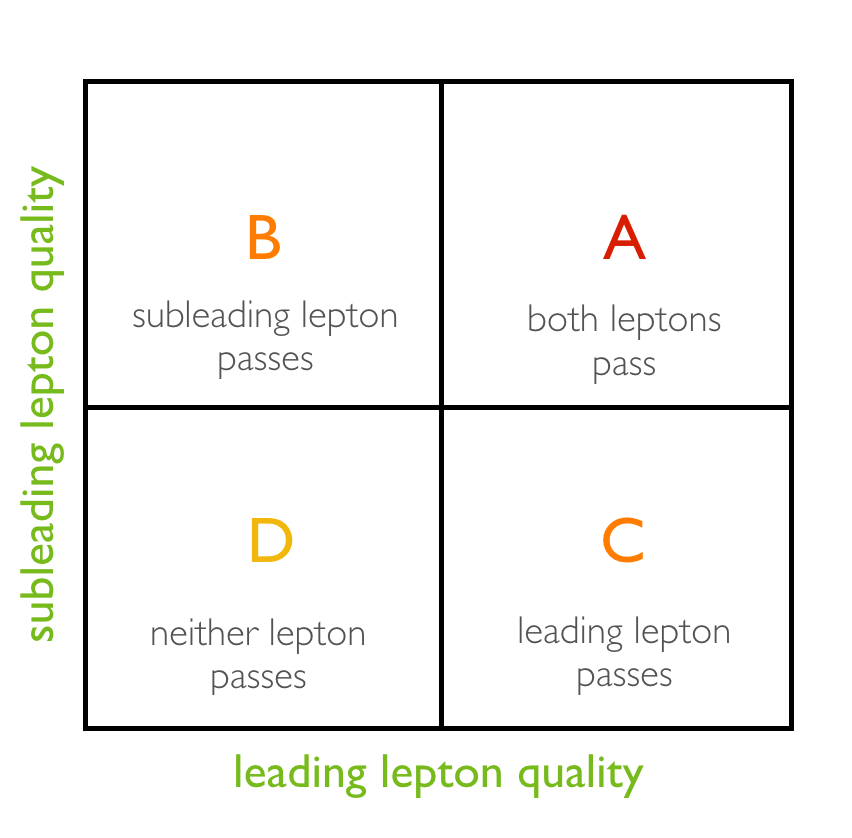
\includegraphics[width=.5\textwidth]{figures/otherbackgrounds/abcd.png}
\caption{The regions used for ABCD estimation.}
\label{fig:abcd}
\end{figure}


In the nominal estimate, region A is the signal region, with two electrons passing all signal cuts, region D has both electrons failing at least one signal cut, and regions C and D have only one electron passing all signal cuts while the other fails at least one (regions B, C, and D compose CR-$ee$-fake). For this estimate, a ``failing'' electron fails one of the \dpt, \chiID, or \nmiss requirements, while a ``passing'' electron is a signal electron, passing all three cuts. The number of events in each region and the estimated number of events in SR-$ee$ is shown in \autoref{tab:abcd_ee}.

\subsection{Validation and Systematic Uncertainties}
The definitions of the ABCD regions can be varied to perform validations of the estimate and quantify systematic uncertainties. There are two ways to do this: first, the estimate can be done in slightly different ways, and the difference from the nominal estimate taken as an uncertainity; second, an estimate can be done in a validation region, where one or more signal cuts are inverted, and the estimated number of events can be compared to the actual number of events in region A. In the second scenario, one looks for \emph{closure}, that the estimate correctly estimates the number of events (within statistical uncertainties), giving evidence that the method and its assumption are sound. If this is not the case, the \emph{nonclosure}, the extent to which the estimate disagrees with the correct number of events, is evaluated and an uncertainty can be taken to cover this.

\begin{table}[htb]
\small
\begin{center}
\begin{tabular}{lcc}
Region     & Nominal            & Only \dpt   \\
\hline
D Observed & 9068         & 1440      \\
C Observed & 77           & 28      \\
B Observed & 54           & 19      \\
A Estimate & $0.459 \pm 0.082$  & $0.37 \pm 0.11$   \\
\hline
\end{tabular}
\caption{Results of the ABCD estimate for the nominal SR-$ee$ estimate, the number of events in each region are shown as well as the estimate for A. The uncertainties are statistical only and using Poisson statistics.}
\label{tab:abcd_ee}
\end{center}
\end{table}

Validations are performed by estimating the number of events in SR-$ee$ in different ways. For example, only the \dpt, the most effective fake discriminator, is used as the ``passing''/``failing'' variable. The results of this estimate are also shown in \autoref{tab:abcd_ee}, the results are consistent within statistical uncertainties but the nominal estimate is more precise.

The second kind of validation is performed in two regions: one that enhances the fake contribution, and a second that enhances the \ac{HF} contribution. First, in a fake enhanced region, VR-$ee$-fake, where the \dpt cut is inverted and the estimate is performed with \chiID and \nmiss together as the ``passing''/``failing'' variables. This changes the estimate to predicting the number of fake electrons (failing \dpt) from regions with electrons that are more fake (failing \dpt and one or both of \chiID and \nmiss). In this region, 1440 events are observed, and 1356 $\pm$ 49 are predicted. Even though this result is consistent within the statistical uncertainties, the difference between the central values (6.2\%) is taken as a nonclosure and applied as a systematic uncertainty on the \ac{SR} estimate.

Next, a validation is done in a \ac{HF} enhanced region, VR-$ee$-fake-hf, which is identical to CR-$ee$-fake with the additional requirement that at least one electron is anti-isolated. This additional requirement reduces the statistics in the region quite a bit, so the electron cuts are loosened to $\pt>50\gev$, $\absdz > 2$ mm, and instead of the usual \dpt cut at -0.5, they must satisfy $\dpt>-0.9$. Electrons in dense environments are more likely to have extra energy added to their clusters or have the wrong track associated, so the \dpt cut must be loosened to probe the subdominant \ac{HF} contribution to the SR-$ee$ background. In this region, $23.5\pm1.9$ events were predicted, and 26 were seen. Again, the results are consistent within uncertainties, with only a 11\% difference in central values. This difference is taken as a systematic uncertainty.

\subsection{Summary}

This estimate is dominated by statistical uncertainties with additional, conservative, systematic uncertainties taken, giving a final estimate of $0.46 \pm 0.10$ (0.082 stat. and 0.058 syst). This estimate has the smallest uncertainty of the three \acp{SR} due to the sufficient statistics in the estimate regions.

\FloatBarrier
\section{Background to SR-$e\mu$}

\subsection{Fake Background}
The background to SR-$e\mu$ is very similar to the background in SR-$ee$ and is estimated in a similar way. By tagging a lepton that fails either isolation or quality requirements and studying the properties of the other, probe lepton, the main contributing background (either fake or \ac{HF}) is determined. Of the probe leptons, 100 pairs failed some signal requirements, but none only failed isolation, indicating that as in the case of SR-$ee$, algorithmic fakes are the dominant background to SR-$e\mu$. 

Fake muons are rare compared to fake electrons due to the lack of extraneous activity in the \ac{MS} compared to the calorimeter where photons add ambiguity to electron reconstruction. As a result, this estimate is extremely statistically limited.

\subsection{Background Estimate}
As in SR-$ee$, the two fake leptons in the event should be uncorrelated and so an ABCD method is used to estimate the background. A ``failing'' electron (as in SR-$ee$) is one that fails any one of the \dpt, \chiID, or \nmiss requirements, a ``failing'' muon fails any one of the  \chiID, \chiCB, \nmiss, \nprecision, or \nphi requirements, and in both cases ``passing'' indicates a signal electron or muon.

However, when performing this estimate, the B region (electron passes, muon fails) has only 1 event, and the C region (muon passes, electron fails) has 0 events. This result cannot be used to calculate a background estimate, but it can be used to place an upper bound by setting the number of events in the C region to 1 event. The total number of events in SR-$e\mu$ must be less than $0.012 \pm 0.017$, where the uncertainty is statistical only. In order to increase the statistical power, different combinations of ``passing'' and ``failing'' leptons were required to only pass the baseline kinematic cuts of $\pt > 50 \GeV$ and $\absdz > 2$ mm. Allowing both passing and failing leptons to only meet the baseline requirements allowed 1 event in the C region, enabling a background estimate of $0.007^{+0.018}_{-0.009}$. Statistical uncertainties are quoted using the Wilson interval for the C/D ratio summed in quadrature with the Poisson uncertainty on the number of events in the B region. This is taken as the nominal upper bound and the full result of this loosening can be seen in \autoref{tab:abcd_loose_em}.

\begin{table}[htb]
\small
\begin{center}
\begin{tabular}{lccc}
Estimate Region     & signal \pt, \absdz cuts  & signal \pt, \absdz cuts  & no signal \pt, \absdz cuts \\
     & on all $\ell$ & passing $\ell$ &  \\
\hline
D Observed                & 81          & 139           & 138     \\
C Observed                & 0             & 0             & 1     \\
B Observed                & 1             & 1             & 1       \\
A Estimate                & $< 0.012 \pm 0.017$   & $< 0.007 \pm 0.010$   & $0.007^{+0.018}_{-0.009}$ \\
%TH NOTE: Numbers are updated with v5.1 ntuples
%Which must pass signal \dz and \pt?  & fail and pass     & pass only       & neither \\
\hline
\end{tabular}
\caption{Results of the ABCD method in the $e\mu$ channel in which the \dz and \pt requirements are selectively loosened from 65 to 50 \gev, and 3 to 2 mm. The first column shows the results without any loosening, the second shows the results with the loosening applied only to the failing leptons, and the final column shows the results with the loosening applied in all regions. Uncertainties are statistical only. For the upper bound results, the value is obtained by setting the C region to 1 event, and the uncertainties are calculated using Poisson statistics. In the final case, the full calculation can be done.}
\label{tab:abcd_loose_em}
\end{center}
\end{table}

\subsection{Validation and Systematic Uncertainties}

As in the case of SR-$ee$, validations are performed enhancing the fake or \ac{HF} contributions. VR-$e\mu$-fake again inverts the most powerful fake discriminators, \dpt for electrons and \chiCB for muons with the loosened \pt and \absdz cuts. In this region, 2 events are observed in the A region compared to $1.9^{+1.8}_{-1.0}$. While these agree within the very large uncertainties, a 7.8\% nonclosure systematic uncertainty is taken from the difference in central values. 

Then, VR-$e\mu$-fake-hf is defined requiring at least one anti-isolated lepton with loosened \pt and \absdz cuts. To increase statistics, the \dpt cut is again loosened to -0.9 and the cuts on \nprecision and \nphi are removed. Here, one event is observed in the A region, and $0.38^{+0.37}_{-0.32}$ events are predicted. To attempt this estimate another way with more statistical power, the estimate is performed again in this region, this time remaining agnostic to whether or not the lepton is isolated. This results in an estimate of $2.6^{+2.0}_{-1.4}$, while 5 events are observed. These numbers are again consistent within their substantial statistical uncertainties, but a conservative 92\% nonclosure uncertainty is taken to account for the difference between the central values.

\subsection{Summary}
This region is extremely statistically limited such that a full background estimate is not possible, and so an upper limit is set. Less than 
$0.007^{+0.019}_{-0.011}$ ($^{+0.018}_{-0.009}$ syst. and 0.006 stat.) background events are expected in SR-$e\mu$.


\FloatBarrier
\section{Background to SR-$\mu\mu$}

\subsection{Cosmic Muon Identification}
\label{sec:cosmics}
Muons from cosmic rays constantly pass through the earth and thus the \ac{ATLAS} detector, particularly through the service shaft above the detector where there is no layer of earth above the detector. If a cosmic ray muon were coincident with a bunch crossing, the event could be triggered, reconstructed, and enter the dataset used for this analysis. The cosmic ray muon could pass through the entire detector at any distance from the \ac{PV}, interacting with the \ac{ID} and \ac{MS}, and be reconstructed as two muons with high \absdz, passing all quality variables (because the signature comes from a real muon) exactly mimicking the signature of SR-$\mu\mu$. 

%\footnote{The cosmic muon flux at sea level is about 1 $\mu$ per cm$^2$ per minute at sea level. ATLAS is approximately 46 m long and 50 m wide and a single data-taking run lasts 8 hours. That's $10^{10}$ cosmic muons per run! Of course, most of \ac{ATLAS} is more than 50 m underground, which absorbs most of the cosmic muons. A muon from a cosmic ray must also be exactly coincident with a bunch crossing to be triggered and well reconstructed. \todo{Do this better with the flux under ground}}

A very efficient cosmic tag was defined for this analysis to identify and remove muons from cosmic rays. This is done using a reoptimization of the strategy used by Ref~.\cite{dvplusmu}. This method first defines a spatial cosmic identification, and then conservatively tags all muons which would be impossible to identify using this method due to gaps in detector coverage. The cosmic muon, \mcos, passes through the entire detector and gets reconstructed as two muons, one on the top of the detector ($\phi > 0$) referred to as \mt and the other on the bottom ($\phi < 0$), called \mb. They follow the relationships 

\begin{equation}
\Delta \phi = |\phi_{\mu_{t}} - \phi_{\mu_{b}}| = \pi 
\end{equation}
and 
\begin{equation}
\Sigma \eta = |\eta_{\mu_{t}} + \eta_{\mu_{b}}| = 0
\end{equation} 

The combination of these variables form a useful variable to describe events with 2 cosmic muons.
\begin{equation}
\Delta R_{\text{cos}} = \sqrt{ ((\phi_{\mu_{t}} - \phi_{\mu_{b}}) - \pi) ^{2} + (\eta_{\mu_{t}} + \eta_{\mu_{b}})^2}
\end{equation}

and it is useful to define
\begin{equation}
\Delta \phi_{cos} \equiv (\phi_{0} - \phi_{1}) - \pi 
\end{equation}

and 


The muon reconstruction algorithm described in \autoref{sec:muonreco} uses the momentum direction measured in the \ac{MS} in its extrapolation from \ac{MS} track to \ac{ID} track and . In 90\% of cases only \mb is reconstructed and identified, while the detector signature for \mt exists but the fully reconstructed muon does not. Thus it is advantageous to tag a cosmic muon as one which is back to back with activity in the \ac{MS}, not as two muons back to back, illustrated in \autoref{fig:tag_sketch}. A cosmic veto is defined based on the \dphicos and \sigeta between a muon and a \ac{MS} segment. 

\begin{figure}[!ht]
\centering
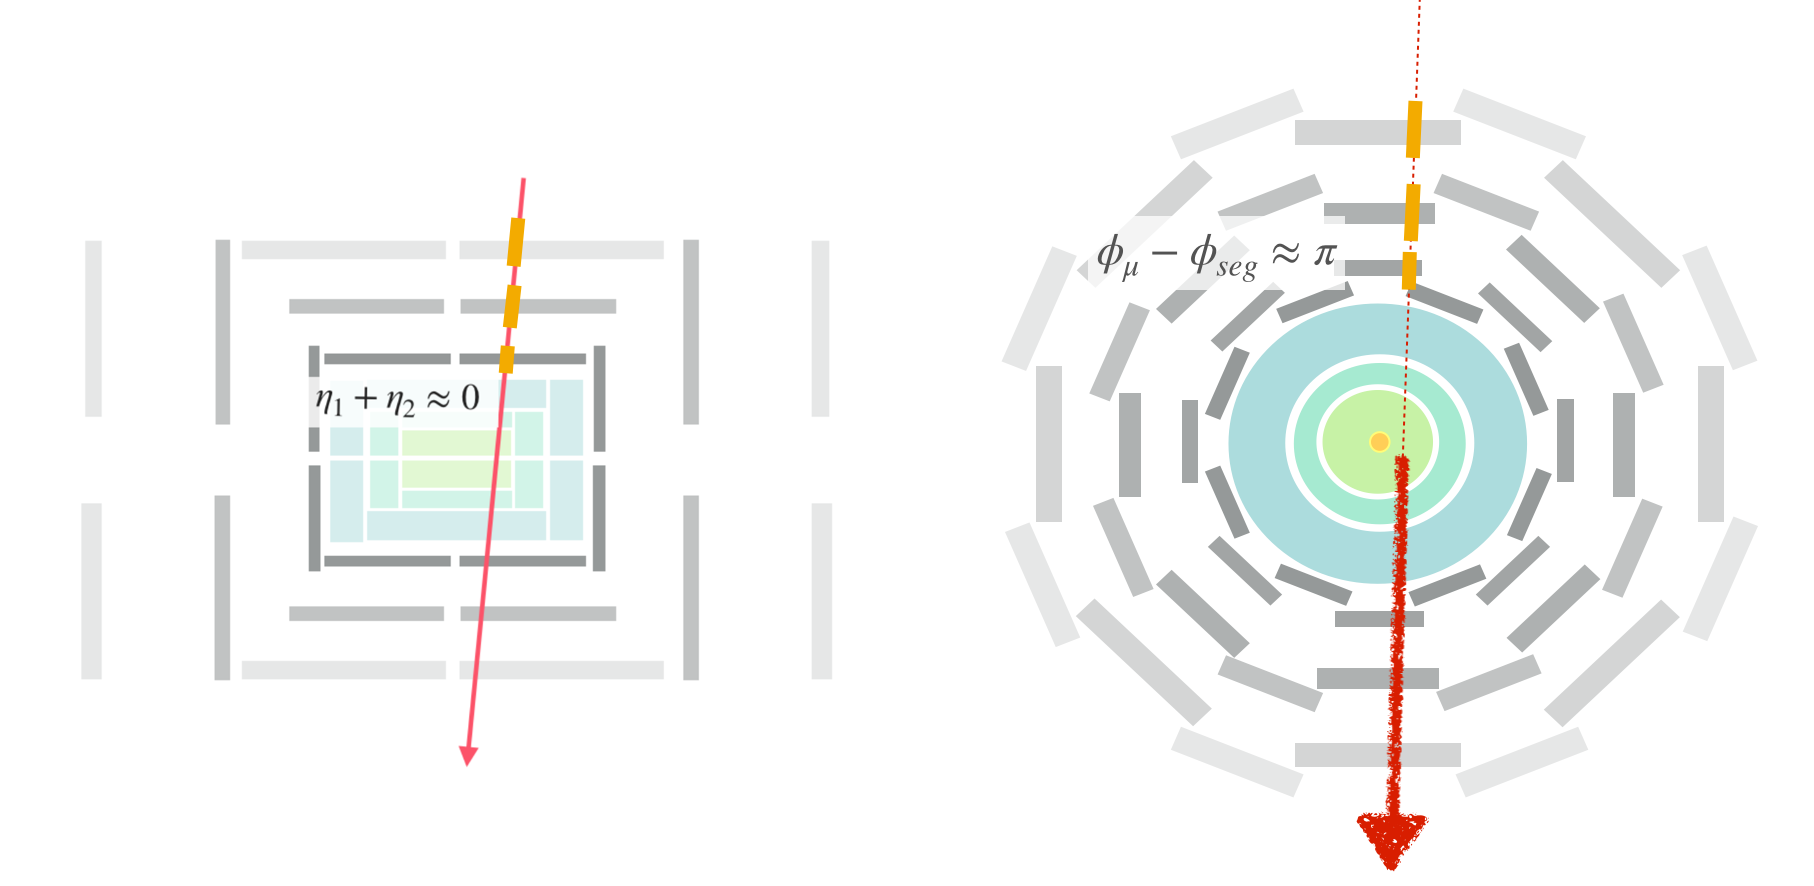
\includegraphics[width=.8\textwidth]{figures/cosmics/tag_sketch.png}
\caption{A sketch of a cosmic passing through the ATLAS detector, illustrating why the tag is designed the way that it is. This image is slightly adapted from Ref.~\cite{dvplusmu}}
\label{fig:tag_sketch}
\end{figure}

Since the \ac{MS} is so far from the \ac{PV}, the \z of individual MS segments is not measured and they are defined to point back to the origin. This creates a mismatch between the $\eta$ of the segment and the $\eta$ of the reconstructed muon in the determination of the cosmic tag. This is geometrically corrected for by re-calculating the $\Delta\eta$ between the segment and the muon in the cosmic veto calculation. A schematic of this correction is shown in \autoref{fig:cos_eta_recalculation}, its effect on the $\eta$ and \sigeta measurements of muons in data is shown in \autoref{fig:changeEta}, and its effect on the \dphicos-\sigeta distribution of cosmic and signal muons shown in \autoref{fig:cos_eta_phi}. This narrows the distribution of cosmic muons by an order of magnitude in \sigeta. This distribution is isotropic for signal muons, so this definition allows for high cosmic muon rejection with minimal signal rejection. 

\begin{figure}[!ht]
\centering
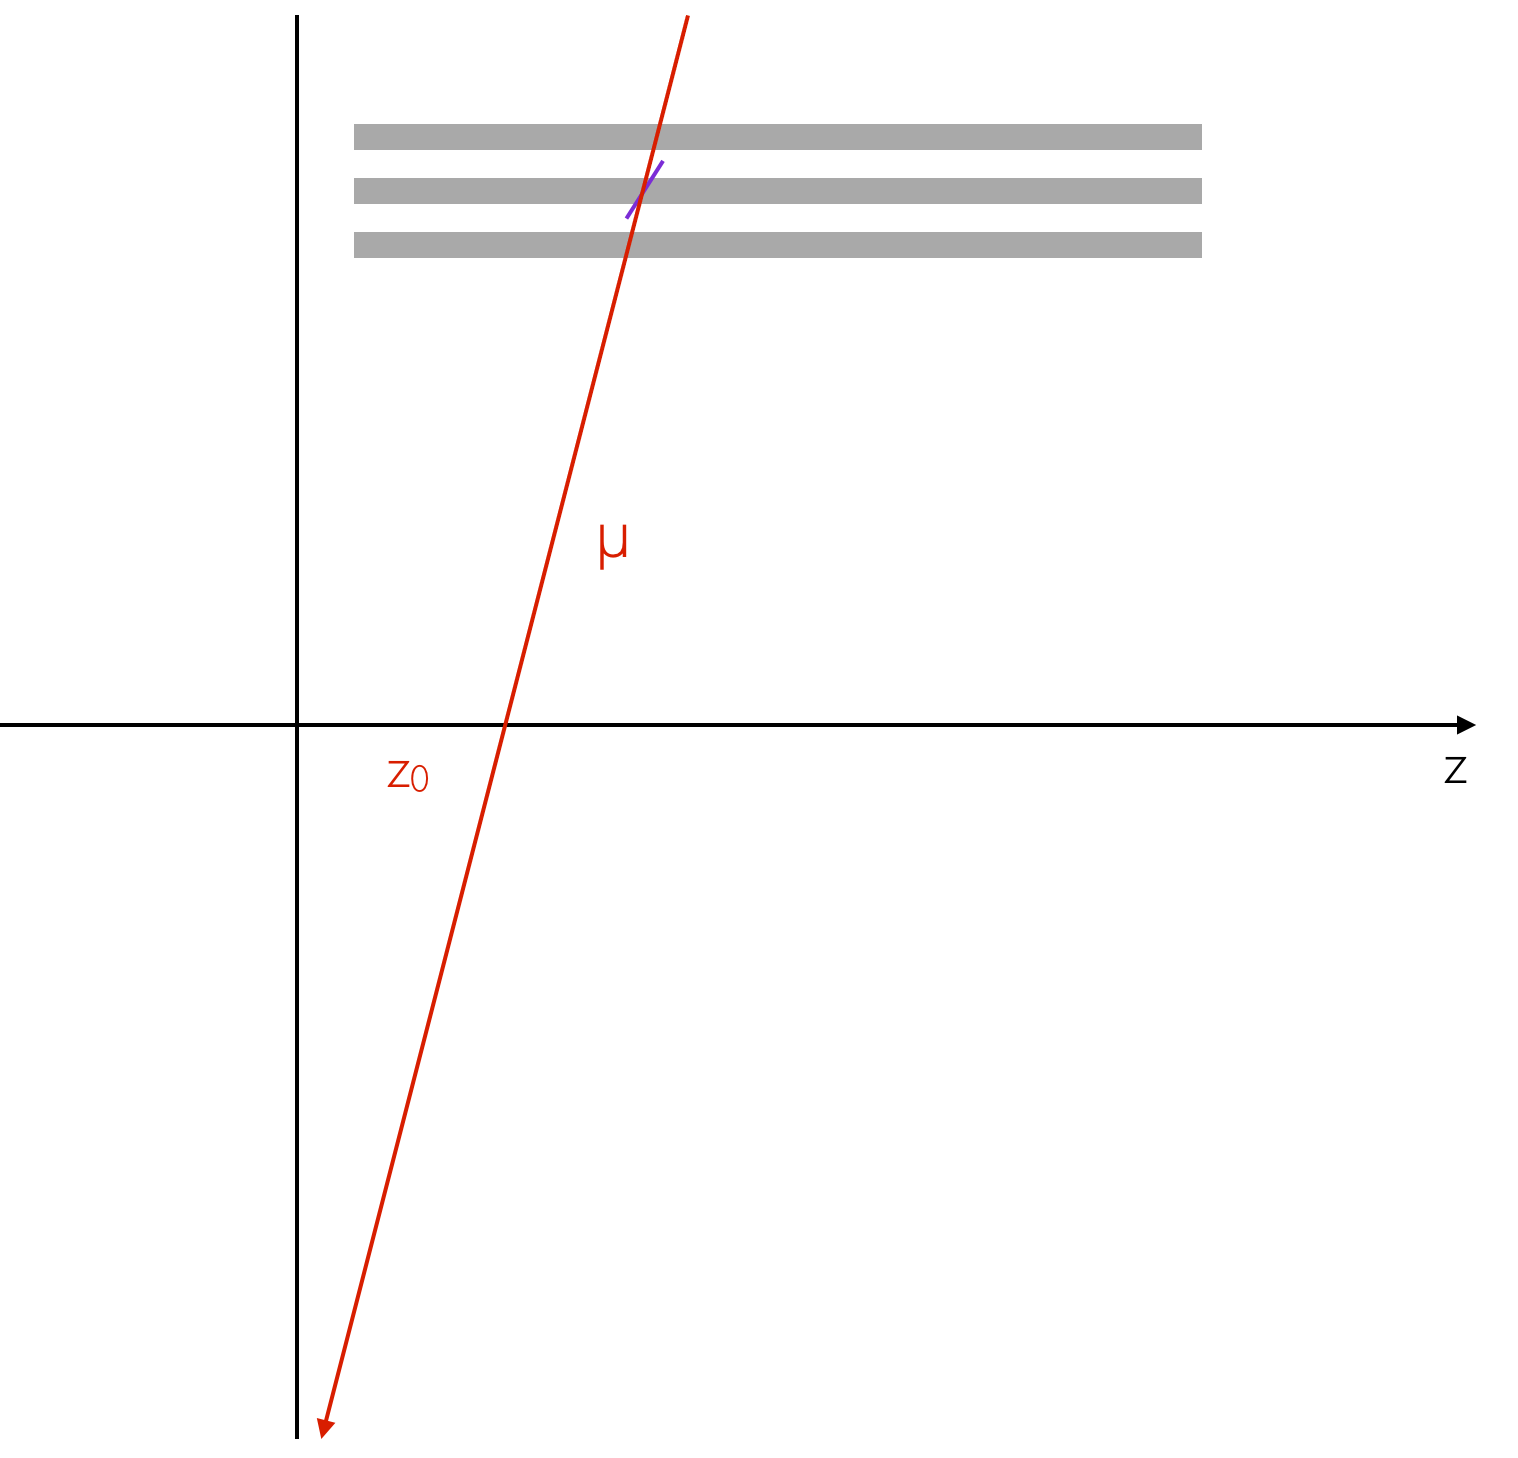
\includegraphics[height=4cm]{figures/cosmics/eta_correction_1.png}
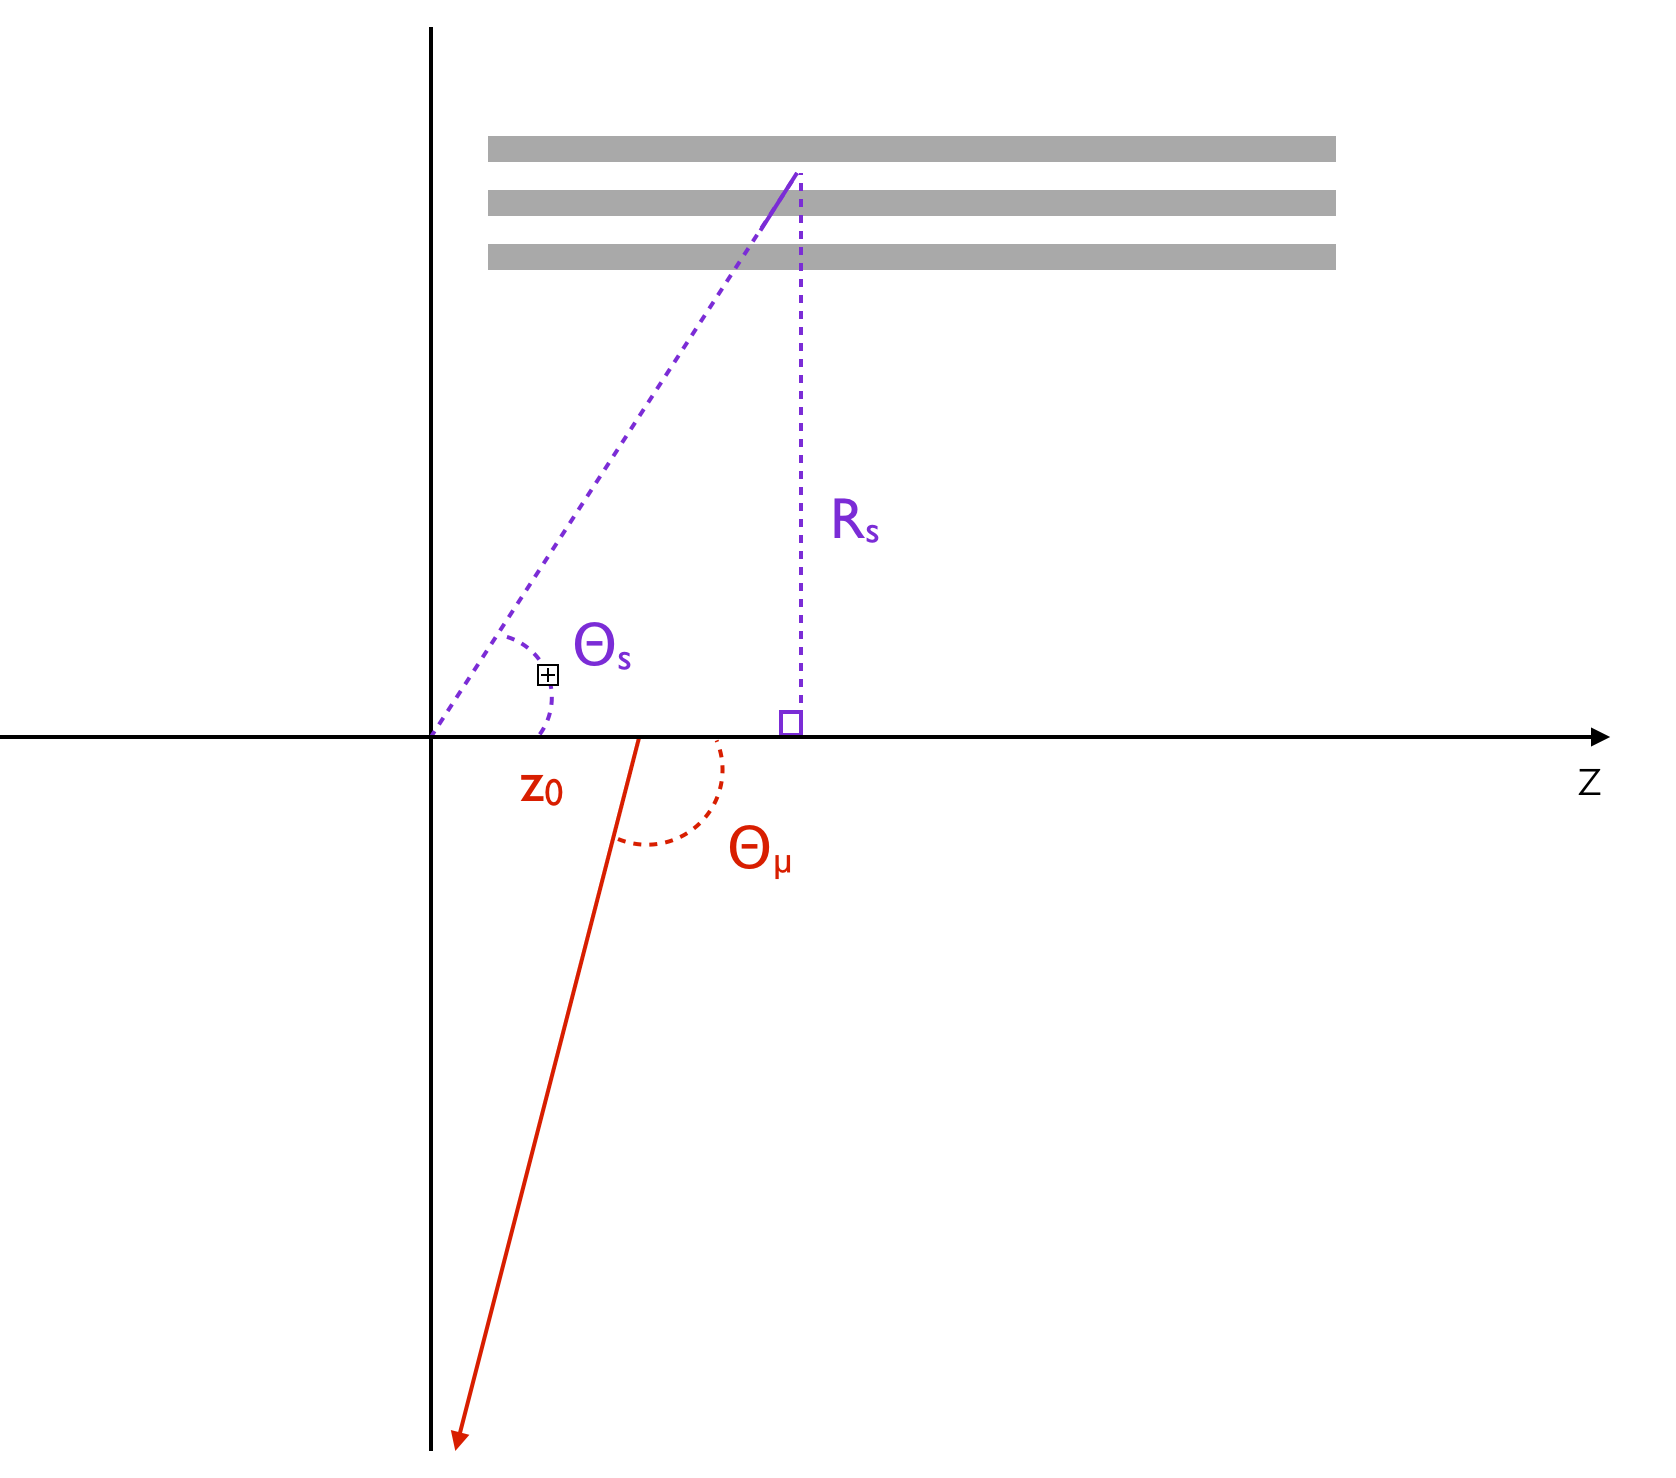
\includegraphics[height=4cm]{figures/cosmics/eta_correction_2.png}
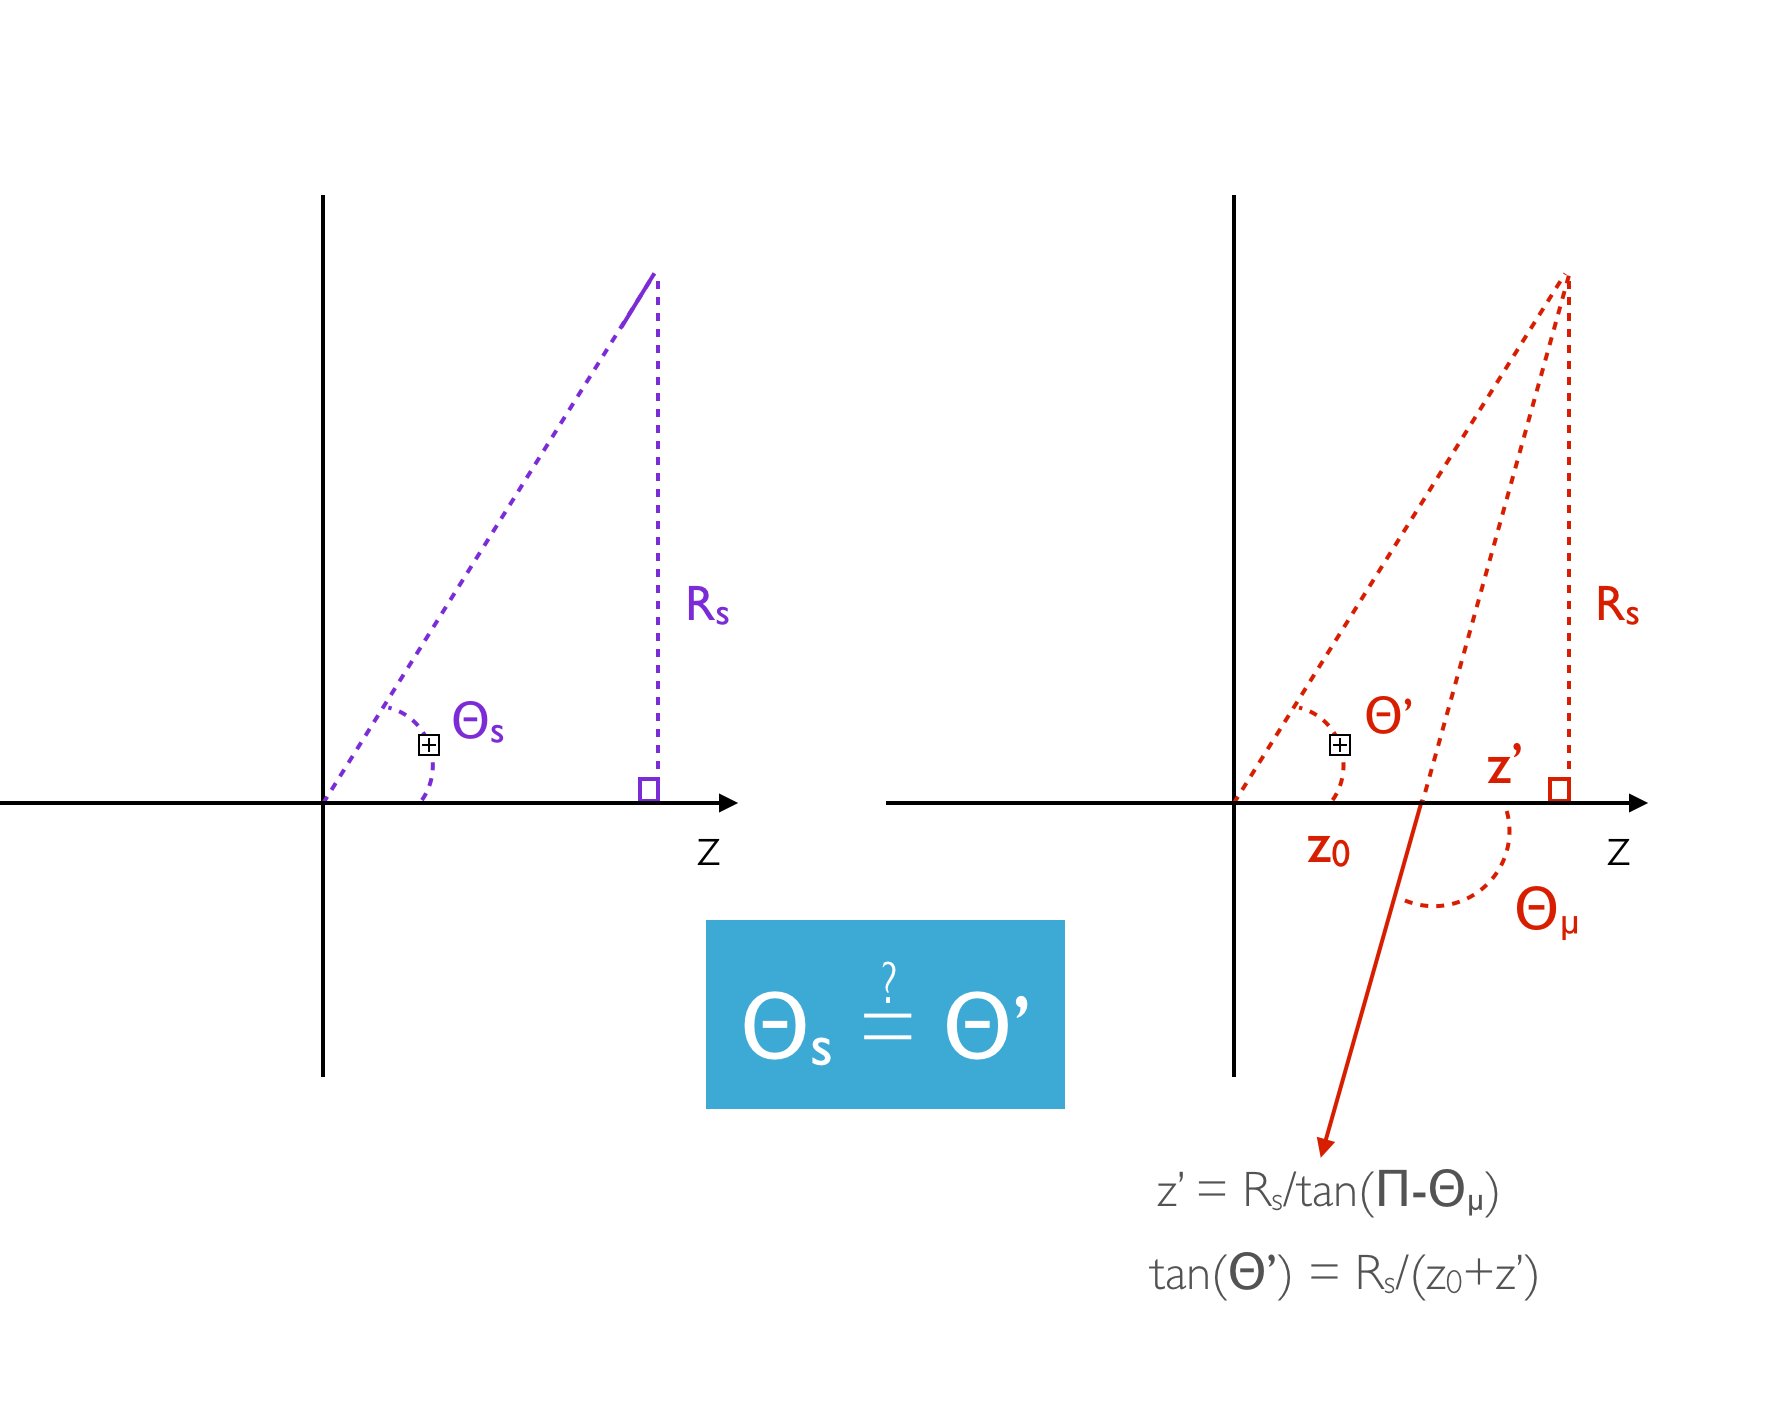
\includegraphics[height=5cm]{figures/cosmics/eta_correction_3.png}
\caption{This series of figures shows the problem of the $\eta$ recalculation. The MS segment should be measured as back to back in $\eta$ and $\phi$ with the muon, because it is really one high $p_{T}$ object moving through the whole detector. However, because the MS segments are reconstructed assuming they come from the origin, they will not actually be measured as back-to-back with the muon. The $\eta$ that would be measured by a segment back to back with the muon is calculated, and compared to the $\eta$ of all other segments in the event.}
\label{fig:cos_eta_recalculation}
\end{figure}

\begin{figure}[!ht]
\centering
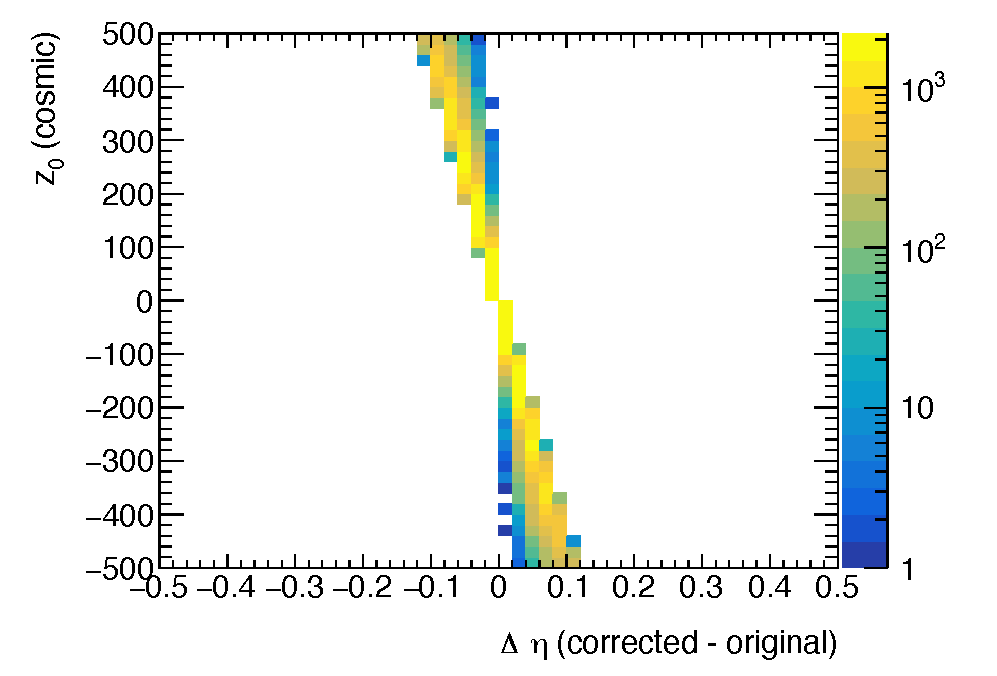
\includegraphics[width=.48\textwidth]{figures/cosmics/cosnotmv_z0_dEta_corr.pdf}
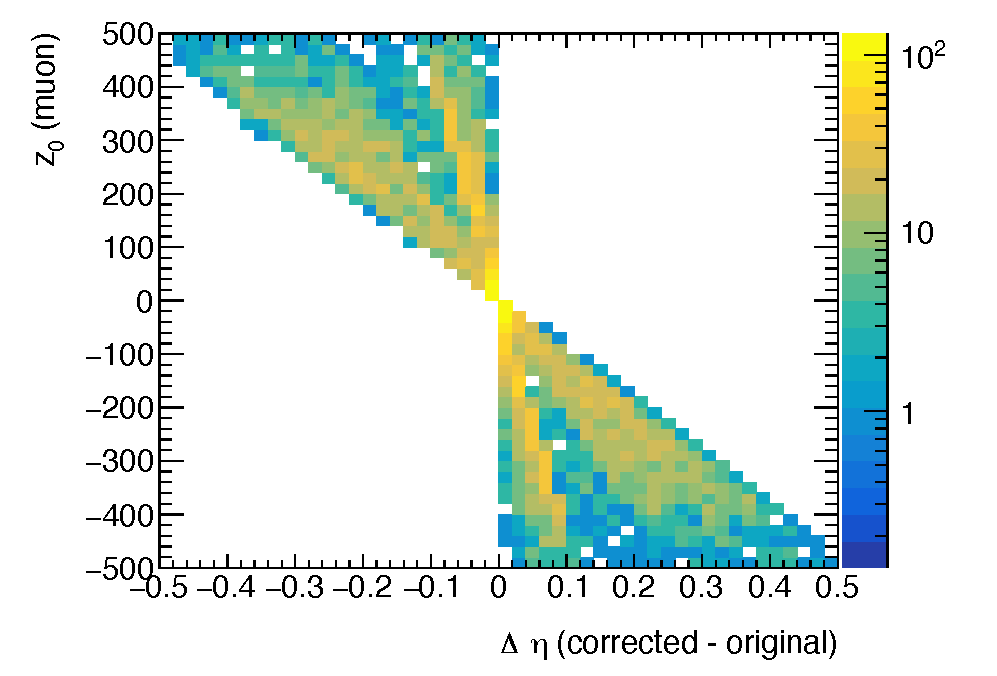
\includegraphics[width=.48\textwidth]{figures/cosmics/mvmu_z0_dEta_corr.pdf}
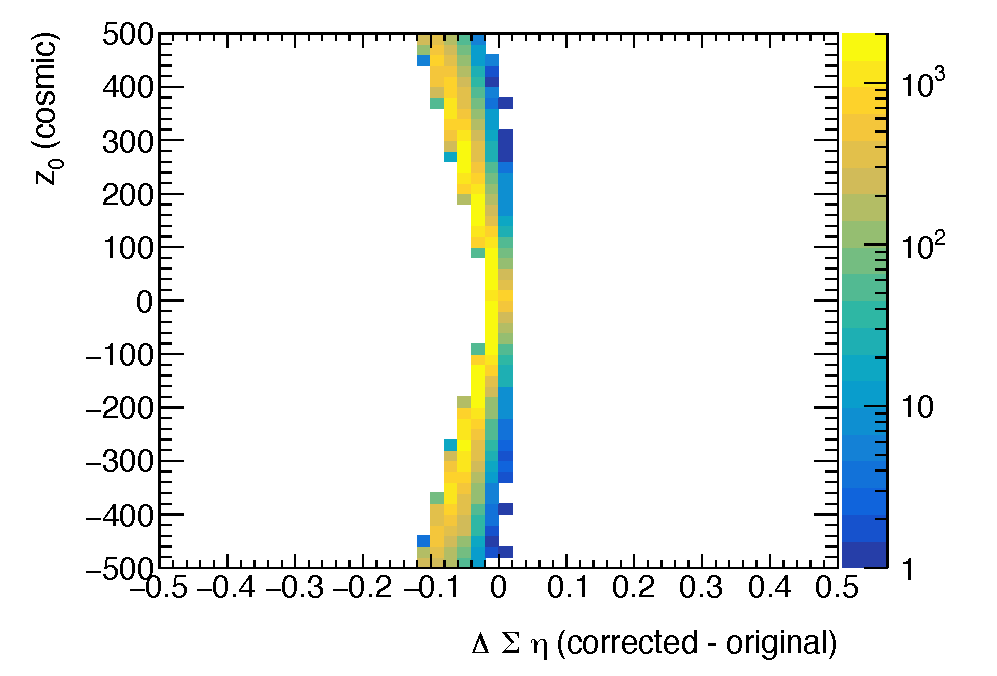
\includegraphics[width=.48\textwidth]{figures/cosmics/cosnotmv_z0_dSeta_corr.pdf}
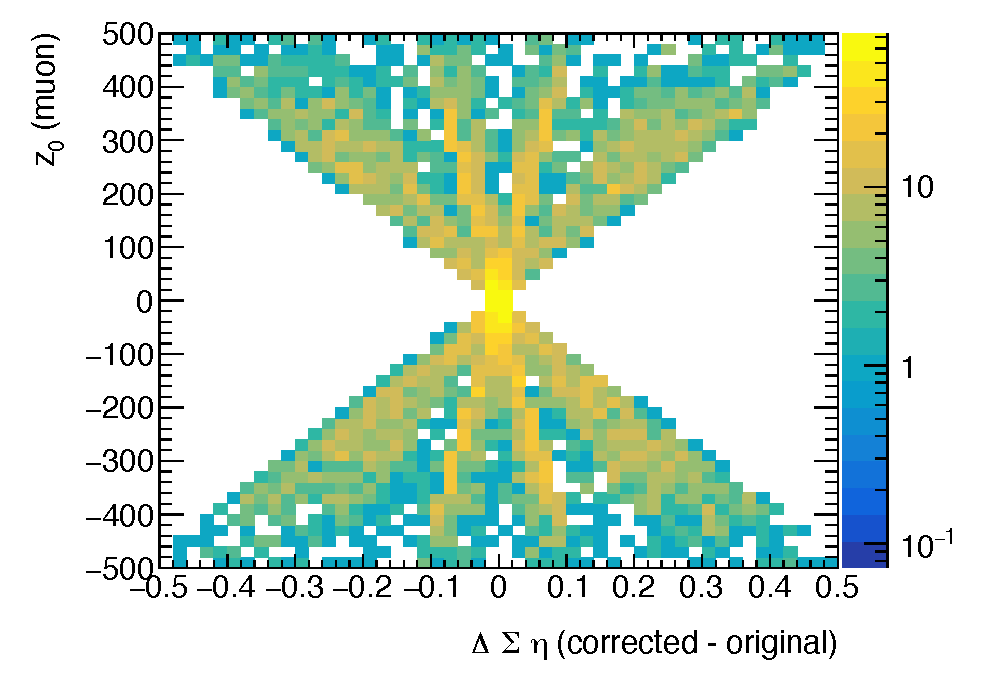
\includegraphics[width=.48\textwidth]{figures/cosmics/mvmu_z0_dSeta_corr.pdf}
\caption{Change to the $\eta$ measurement (top) and \sigeta measurement (bottom) due to the $z_{0}$ correction. These plots compare muons tagged with due to the presences of a segment in the \dphicos-\sigeta window (left) to those untagged or tagged with the detector coverage veto (right). The behavior shows isotropic effect for the muons which are not tagged via the algorithm that uses this correction, while the \sigeta distribution of cosmic muon always decreases due to the correction.}
\label{fig:changeEta}
\end{figure}


\begin{figure}[!ht]
\centering
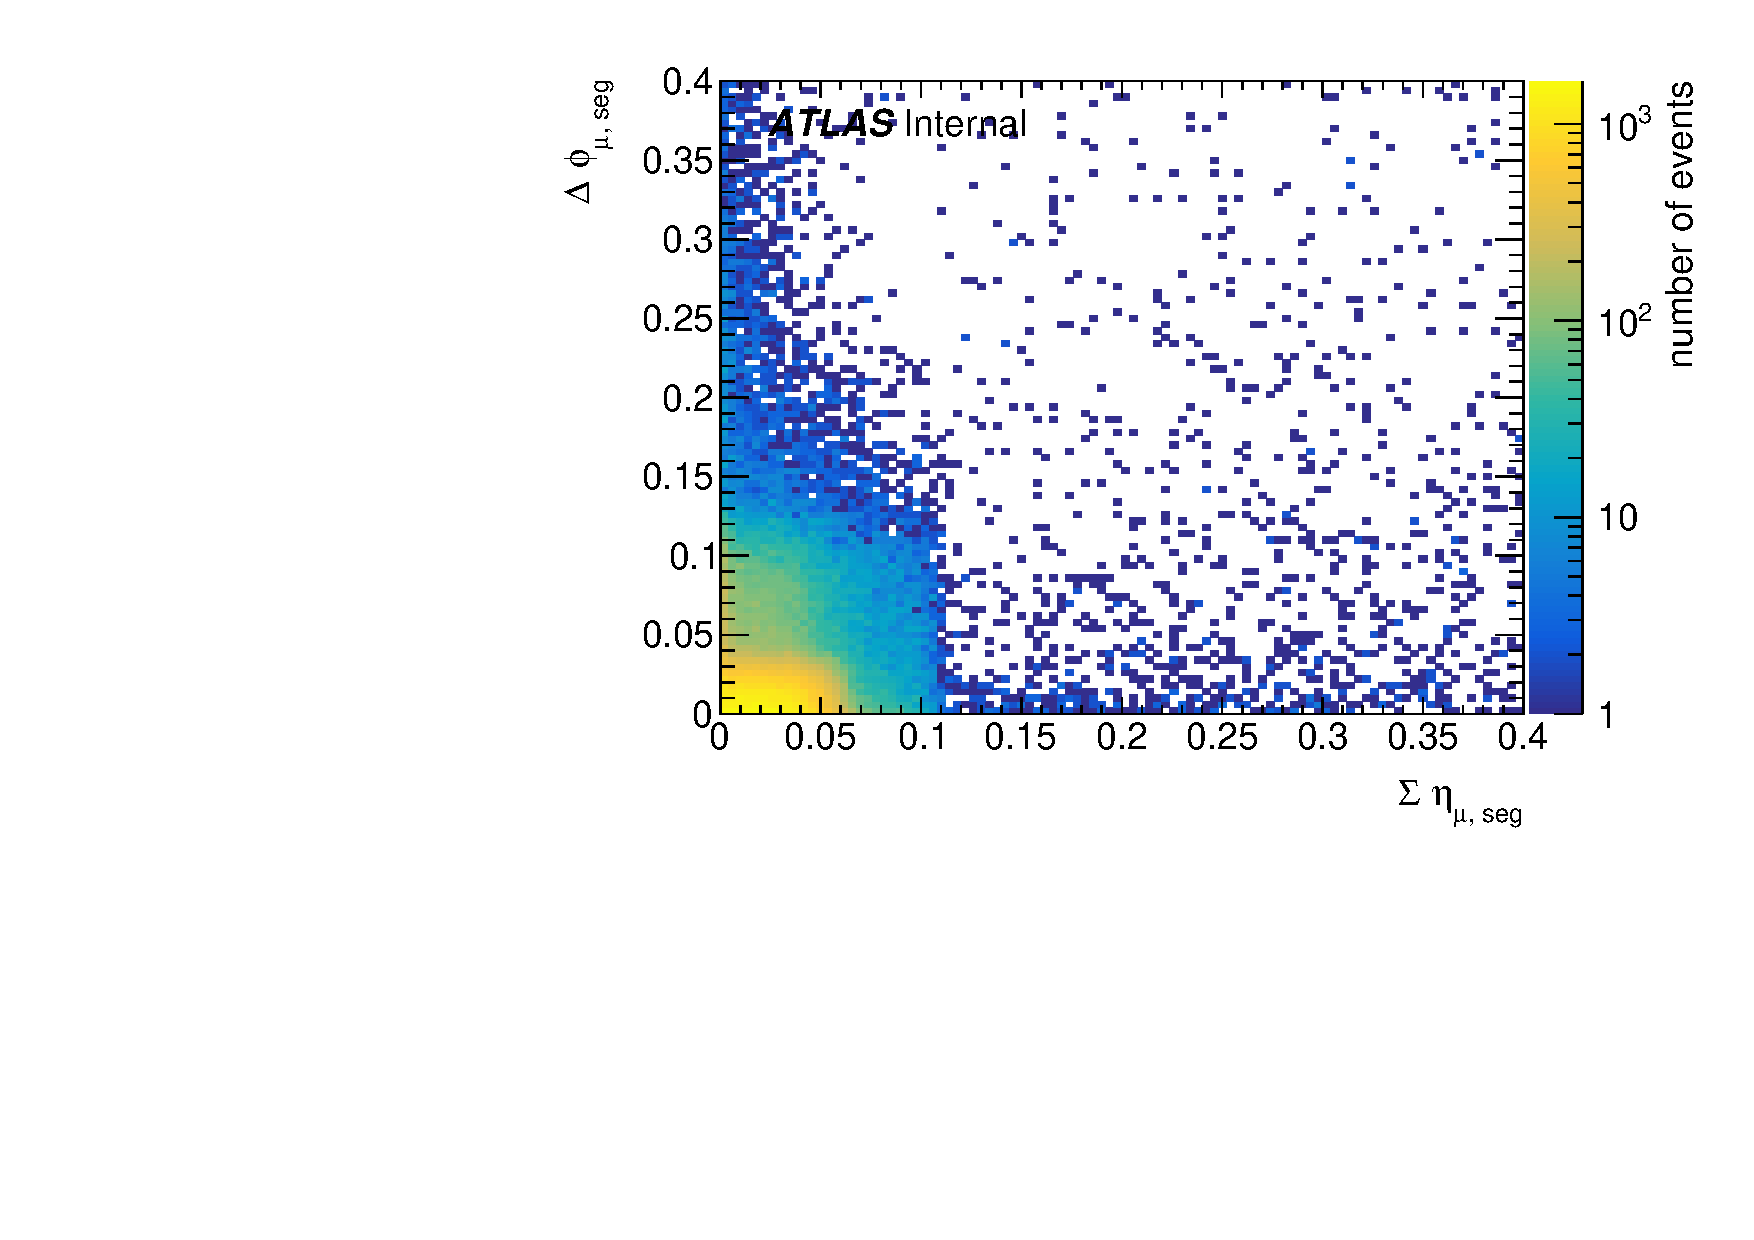
\includegraphics[width=.48\textwidth]{figures/cosmics/v4_widetag_2_sumEta_dPhi_min.pdf}
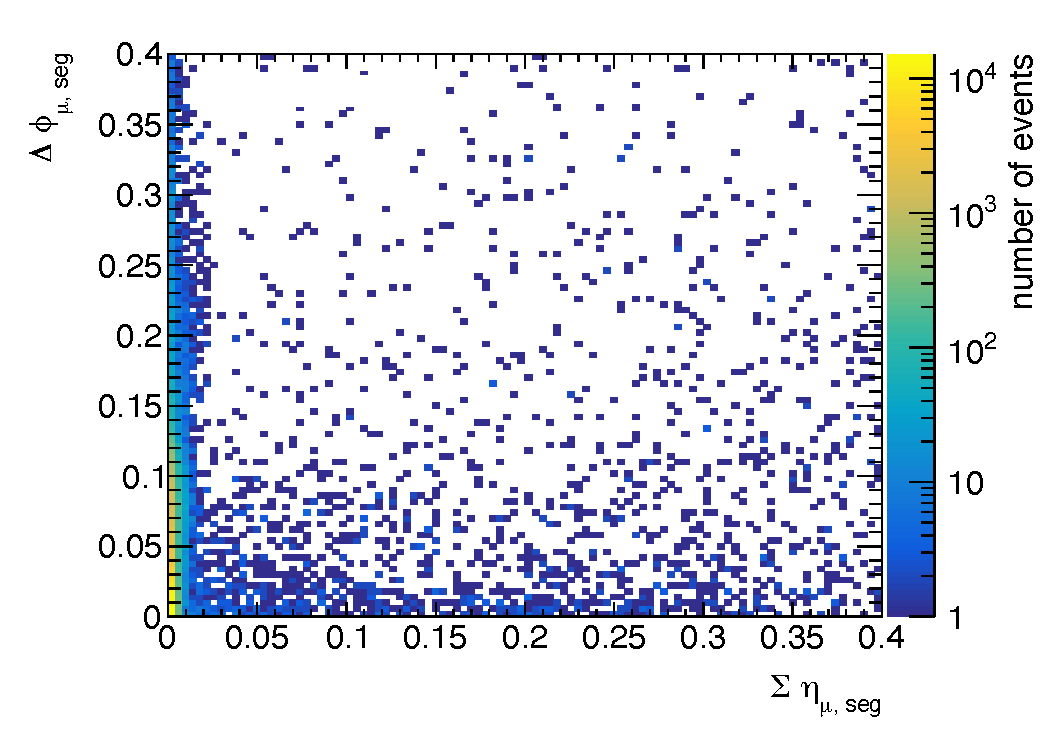
\includegraphics[width=.48\textwidth]{figures/cosmics/v4_widetag_2_sumEta_dPhi_min_corr.pdf}
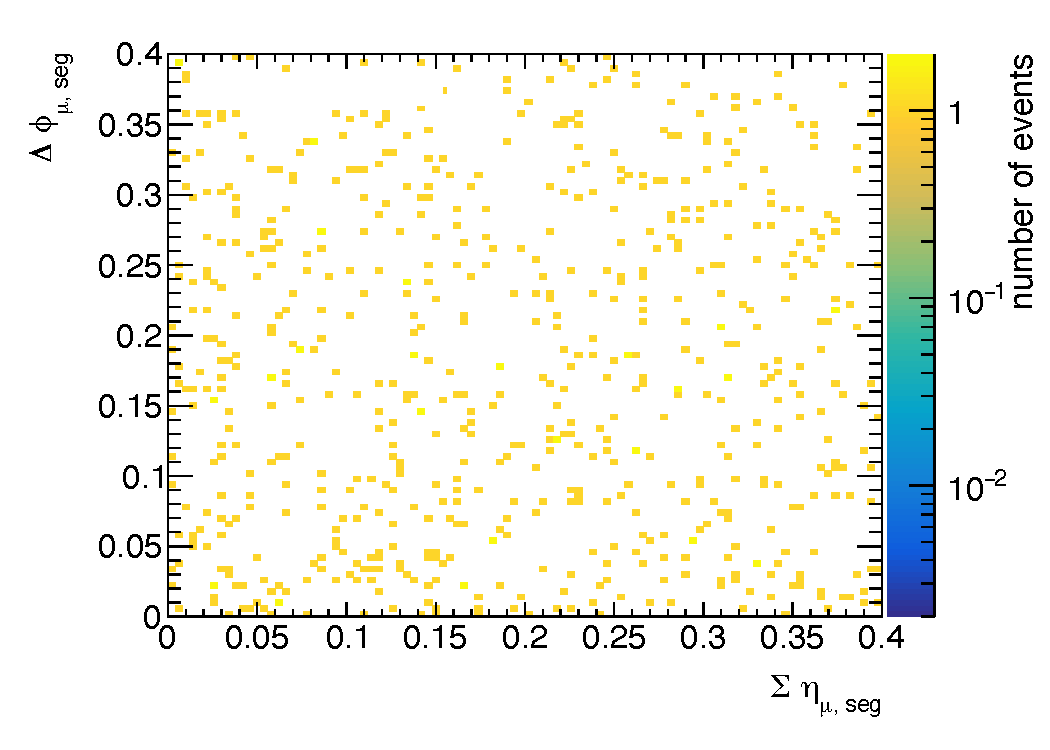
\includegraphics[width=.48\textwidth]{figures/cosmics/300_slep_2_sumEta_dPhi_min.pdf}
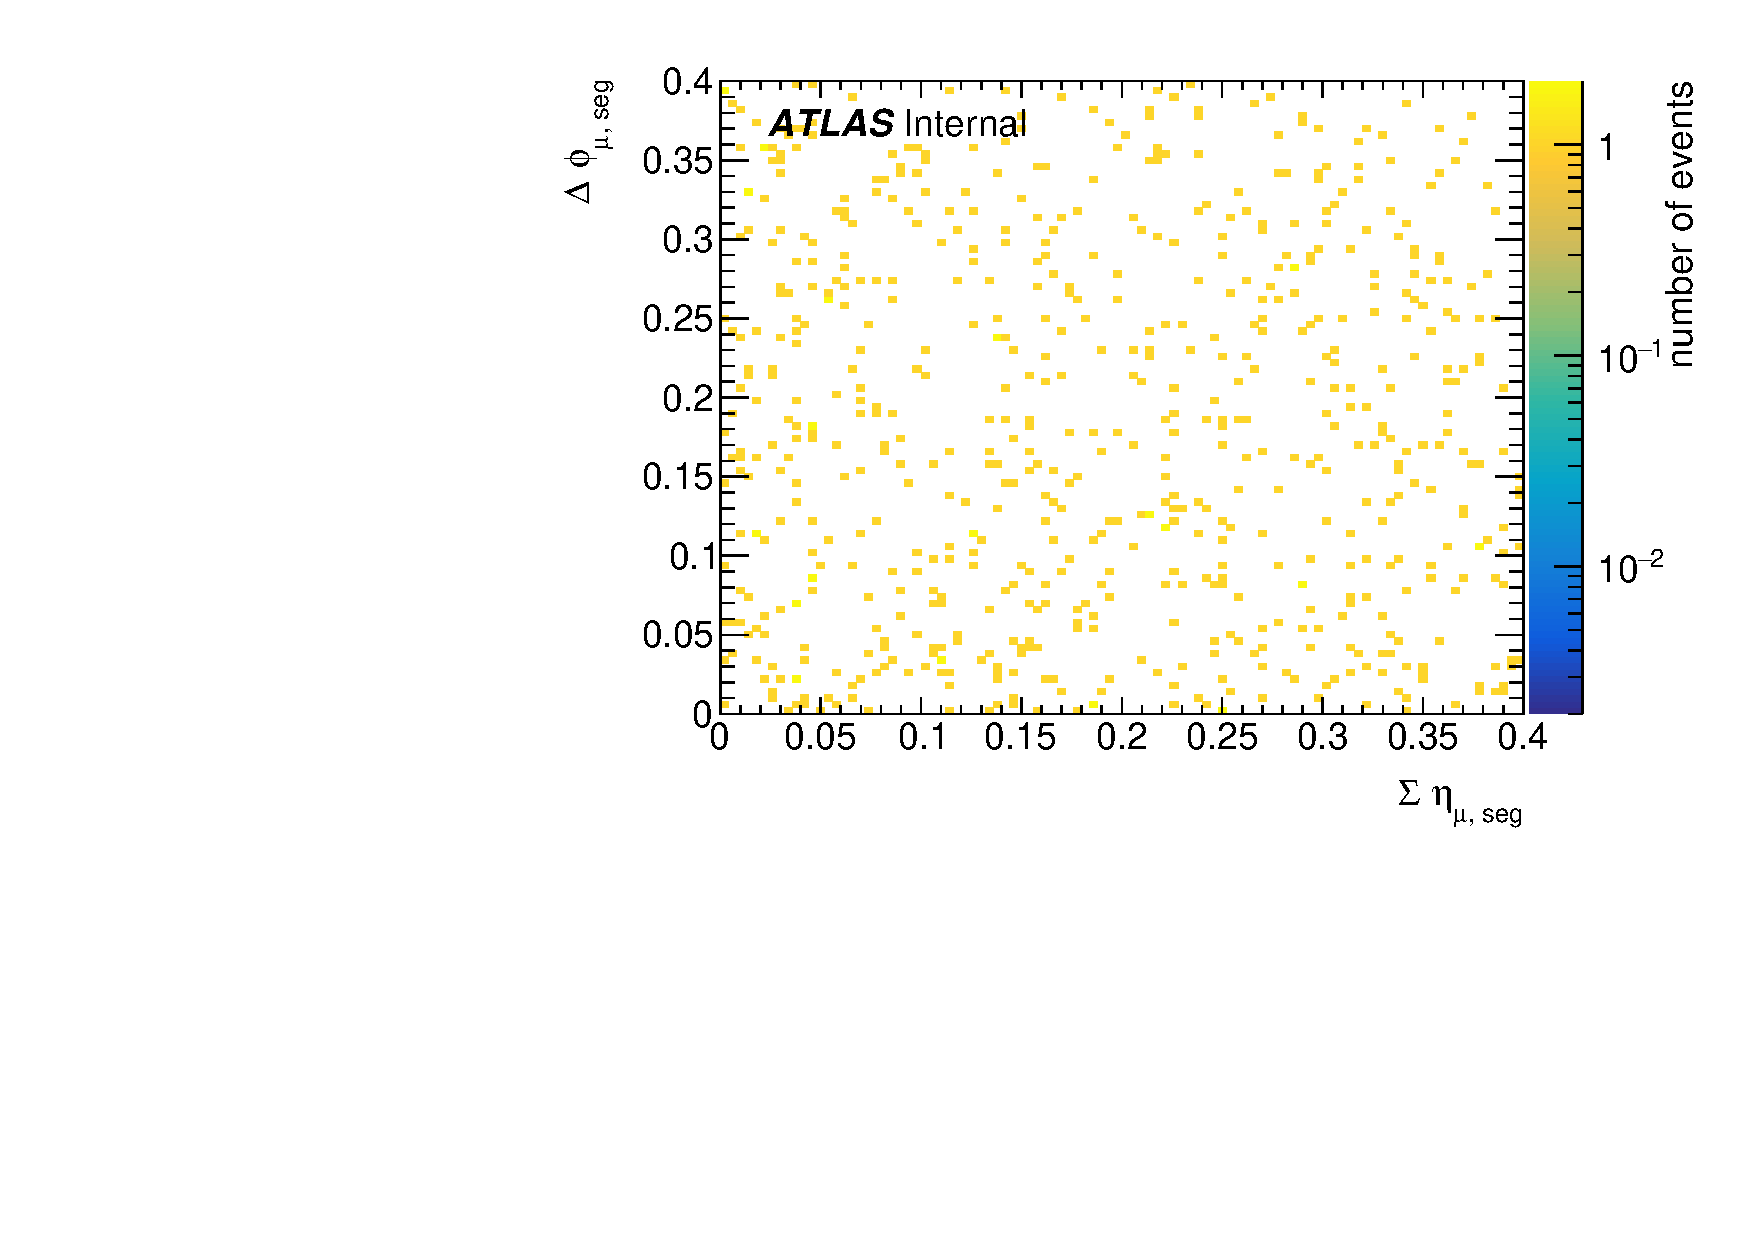
\includegraphics[width=.48\textwidth]{figures/cosmics/300_slep_2_sumEta_dPhi_min_corr.pdf}
\caption{The $\Sigma\eta - \Delta\phi$ distribution is shown before (left) and after (right) the $\eta$ recalculation. The top row shows the distributions in VR-$\mu$ and bottom row 300 GeV \slep signal samples in our full range of lifetimes. Using this cosmic tag, a very tight cut can be made on cosmic muons without losing signal efficiency.}
\label{fig:cos_eta_phi}
\end{figure}


The distribution the $\dphicos-\sigeta$ distribution is much narrower in \sigeta than in \dphicos. This is because the \ac{MS} measures $\eta$ with an extremely high precision in the \acp{MDT} ($\mathcal{O}(10~\um)$), since it is the bending direction of the toroid and thus gives the momentum measurement, while the $\phi$ is measured by the \acp{RPC} with an order of magnitude less precision ($\mathcal{O}(10~\text{mm})$). A high precision $\phi$ measurement of the combined muon comes from the \ac{ID}, but the cosmic tag must contend with these resolution limitations to find a muon segment.

Additionally, there are gaps in the \ac{MS} to allow for detector access, so a muon is conservatively tagged as a cosmic if it is back to back with this gap in detector coverage, as it could not be tagged as a cosmic using the geometric algorithm. A map of the material of the \ac{MS} is used to veto cosmic muons using this \emph{detector coverage veto}. \autoref{fig:cos_material_veto} shows the impact of each step on the muon distribution in VR-$\mu$, which is dominated by muons from cosmic rays.


\begin{figure}[!ht]
\centering
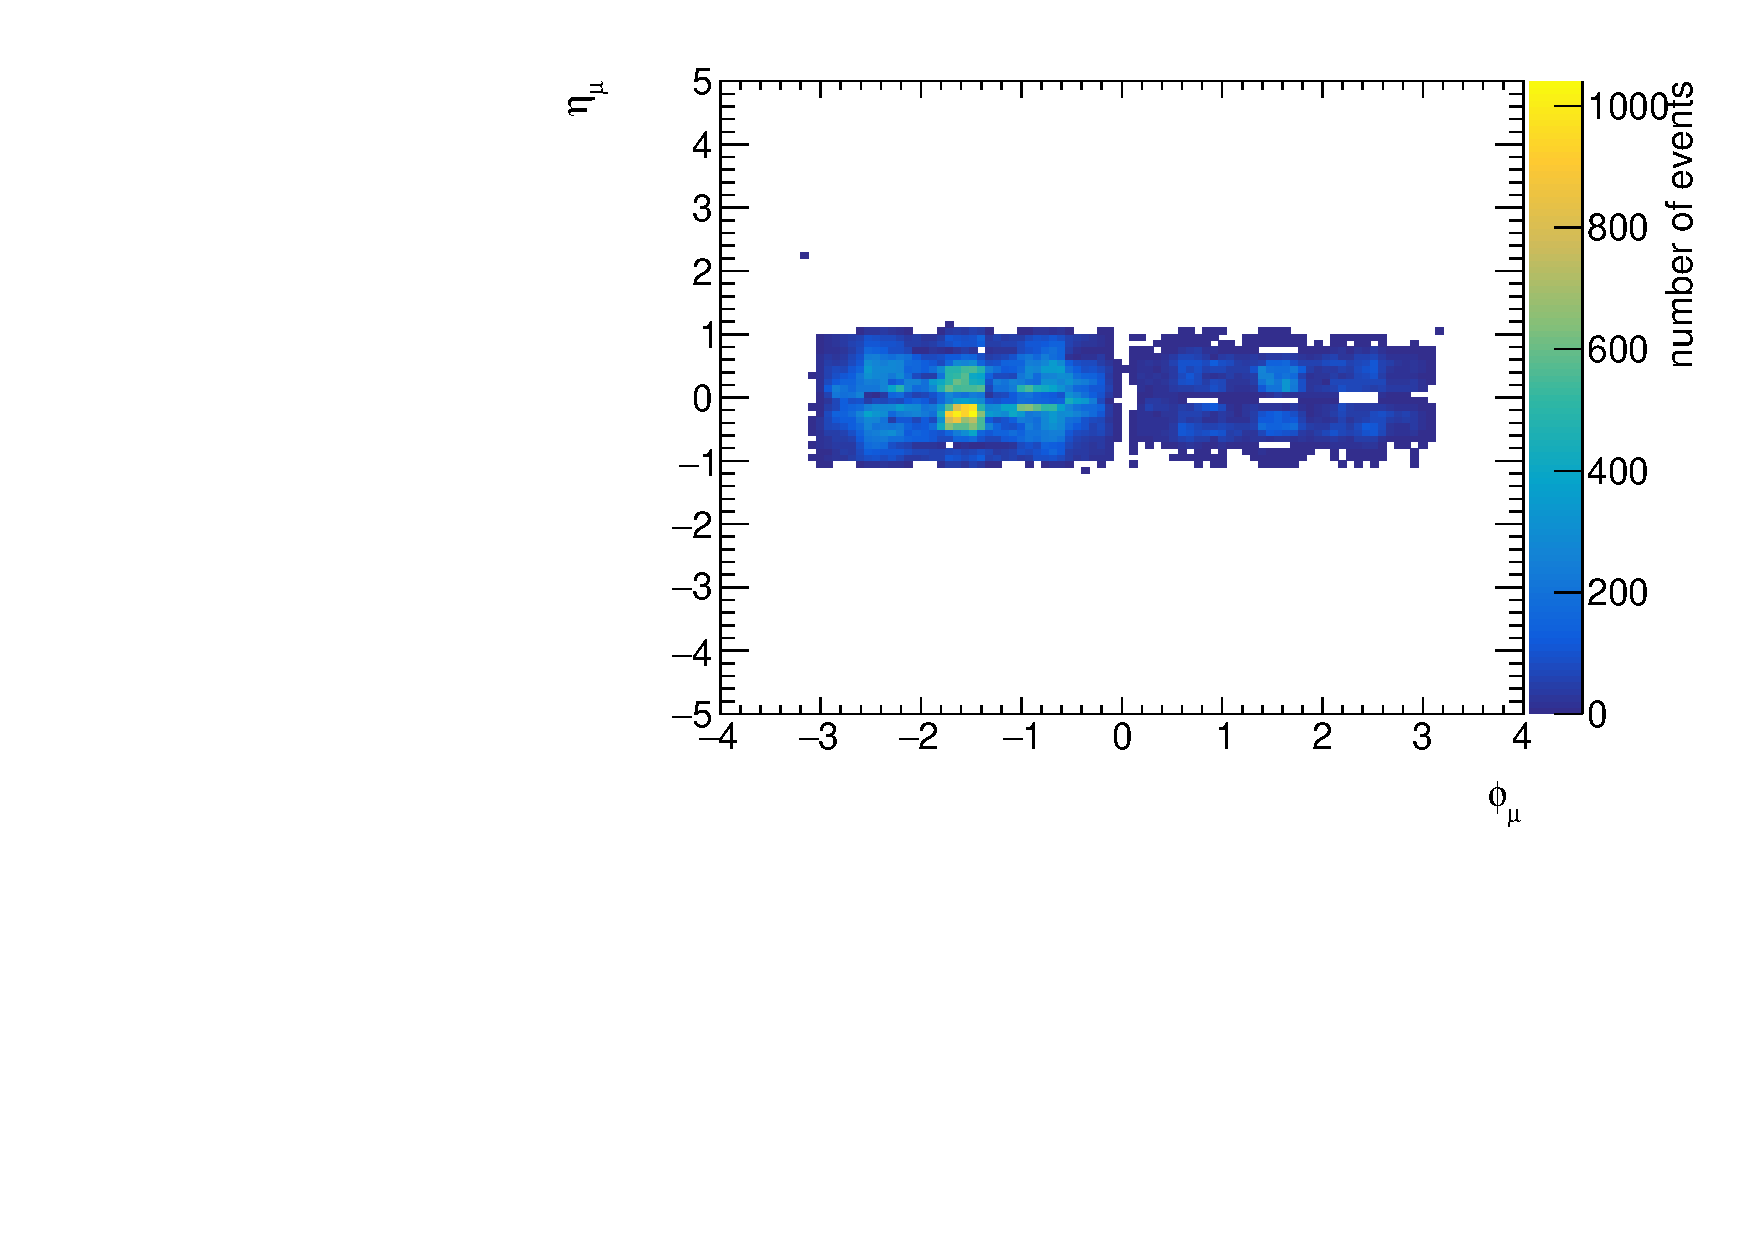
\includegraphics[width=.48\textwidth]{figures/cosmics/v4_widetag_2_eta_phi_baseline.pdf}
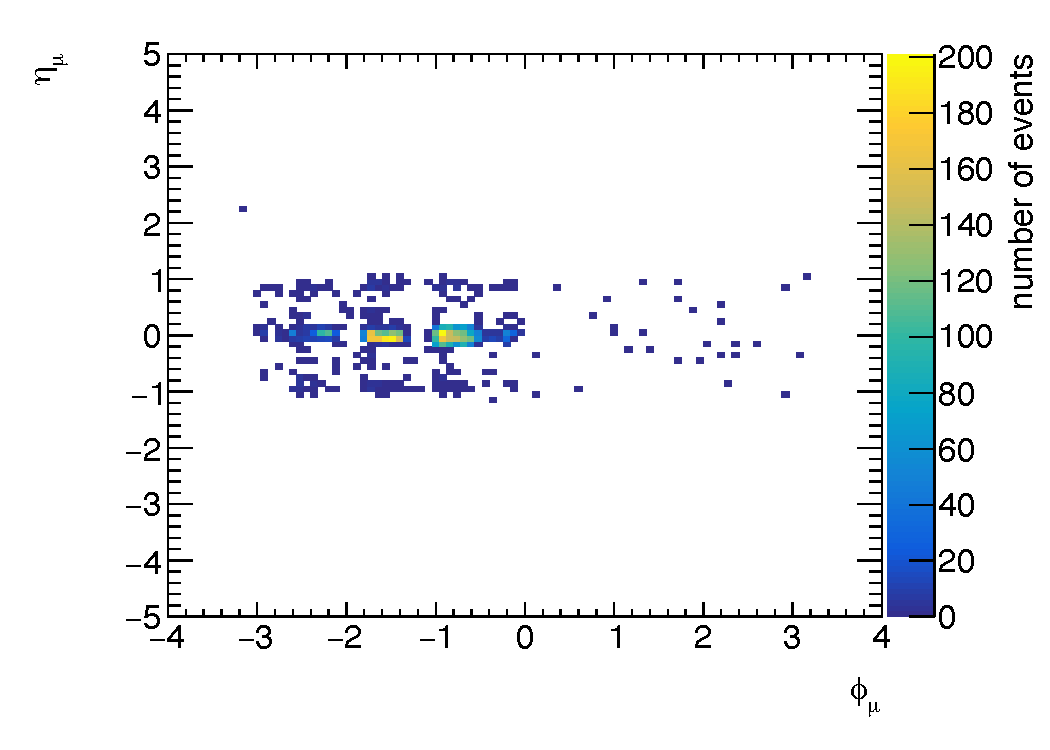
\includegraphics[width=.48\textwidth]{figures/cosmics/v4_widetag_2_eta_phi_costag.pdf}
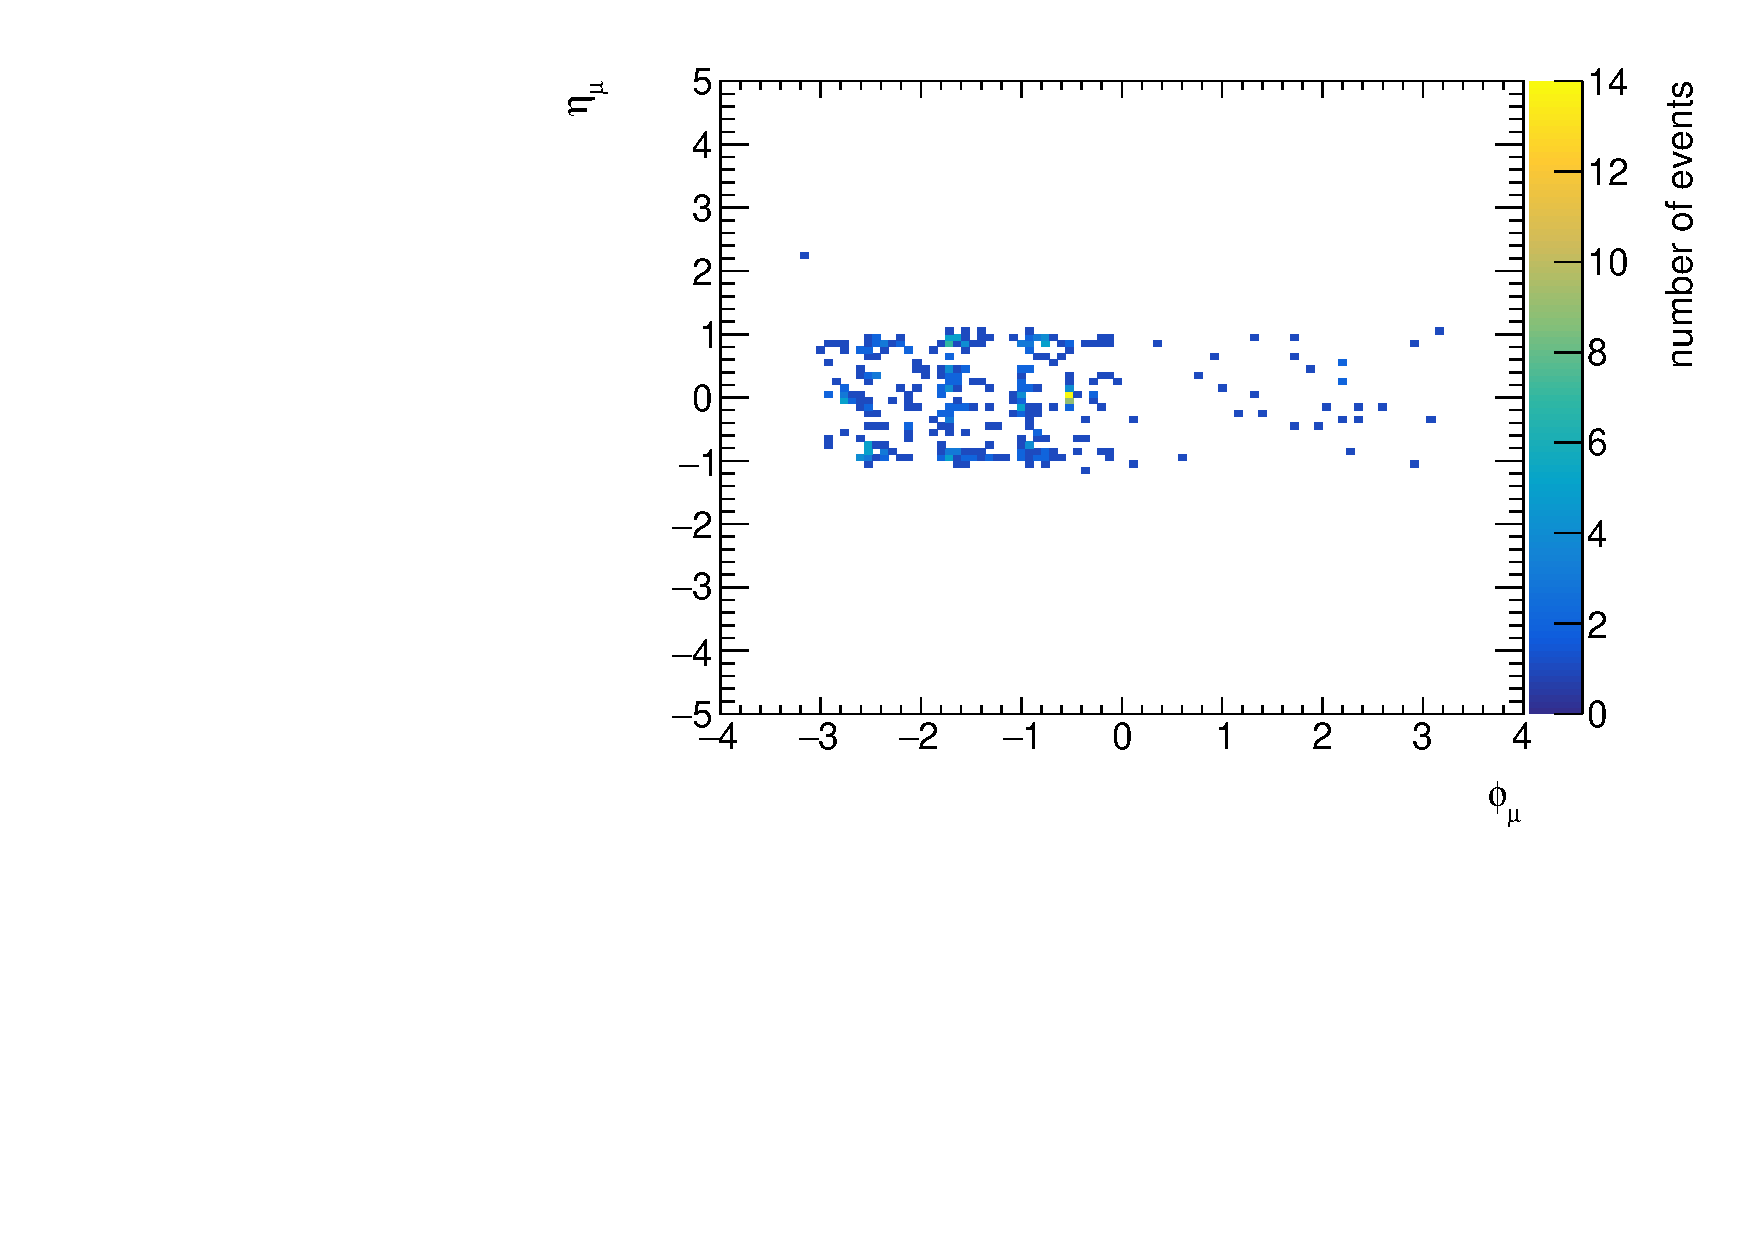
\includegraphics[width=.48\textwidth]{figures/cosmics/v4_widetag_2_eta_phi_costag_mv.pdf}
\caption{The $\eta-\phi$ distribution of muons in VR-$\mu$ are shown after baseline cuts (top left), the cosmic veto (top right), then the detector coverage veto (bottom).}
\label{fig:cos_material_veto}
\end{figure}

For this analysis, two different definitions of a ``cosmic muon'' are used. The \emph{nominal tag} is used to veto events in the \ac{SR}. If any baseline muon is tagged by the nominal cosmic tag, the entire event is vetoed. A second \emph{narrow tag} is used during the validation of the estimate of background from cosmic muons. Both tags require muons to pass the detector coverage veto. \autoref{tab:costag_values} describes the values used for the various cosmic tags used and \autoref{fig:cos_tag} shows the cuts used in the \dphicos-\sigeta distribution. 

\begin{figure}[!ht]
\centering
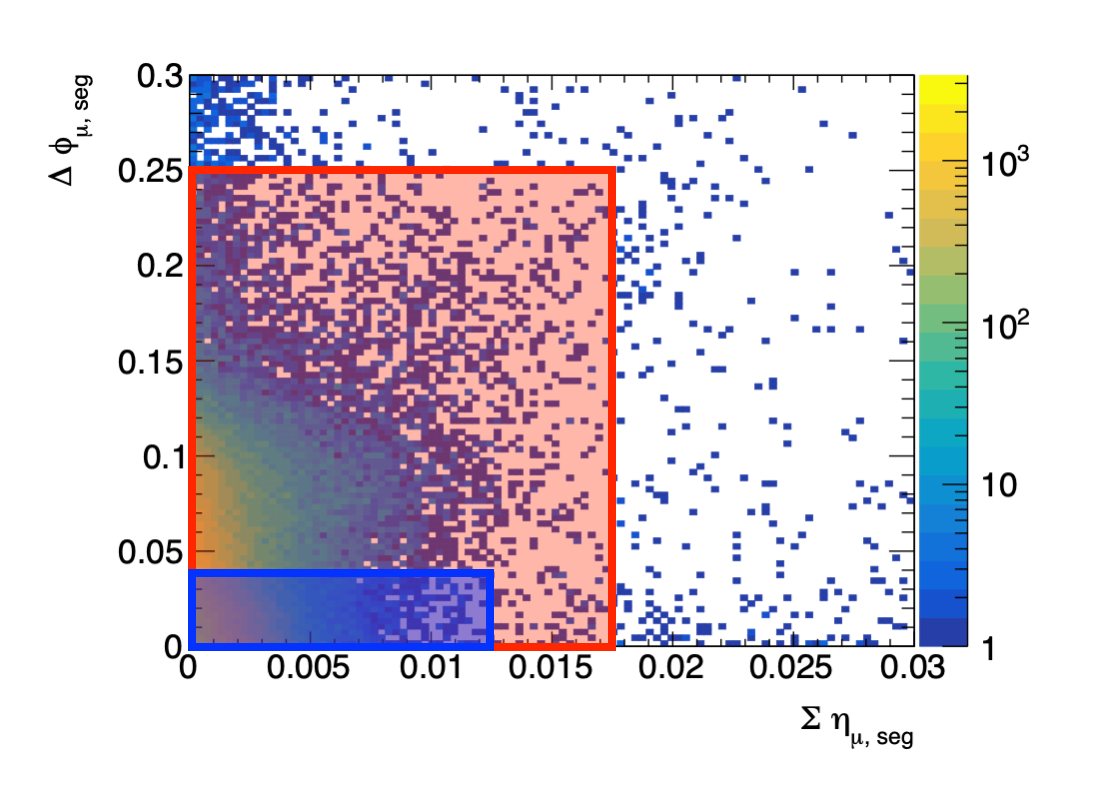
\includegraphics[width=.48\textwidth]{figures/cosmics/cosmic_tag.png}
\caption{The $\Sigma\eta_{\mu,\textrm{seg}} - \Delta\phi_{\mu,\textrm{seg}}$ distribution of signal quality muons in VR-$\mu$. The red line and shadow shows the bounds of the full cosmic tag, while the blue line and shadow shows the boundary of the narrow cosmic tag. Everything inside the respective boxes is tagged as a cosmic. The intermediate tag defines the region included in the full tag, but not included in the narrow tag.}
\label{fig:cos_tag}
\end{figure}

\begin{table}
\centering
\begin{tabular}{lcccc}
Tag & $\Delta \phi (\mu, \textrm{seg})$ & $\Sigma \eta (\mu, \textrm{seg})$ & Pass Coverage  & Rejection \\
 &                                         &                                &    Acceptance & Efficiency \\
\hline
Full   & $<0.25$   & $ <0.018 $   & True & 99.5\% \\
Narrow & $<0.02$   & $ <0.013$    & True & 59\% \\
\hline
\end{tabular}
\caption{Cuts applied in full and narrow cosmic tags. The narrow is contained in the full tag. An intermediate tag is defined as the region between the full and narrow tags, that is, tagged by the full but not the narrow tag.}
\label{tab:costag_values}
\end{table}

The cosmic tagging efficiency is determined by fitting distributions in VR-$\mu$. A template of the \tavg of cosmic tagged muons and prompt (collision) muons is taken from data shown on the left of \autoref{fig:d0_t0avg}. Any correlation between \tavg and \dz can not be observed within detector resolutions, so the prompt sample of muons is taken to represent the signal muons that would result from collisions.

These are used to determine the fraction of cosmic muons in VR-$\mu$ before and after the cosmic tagged muons are removed from VR-$\mu$ (left of \autoref{fig:d0_t0avg}). From the fraction of cosmic muons estimated from the template fitting, the fraction of muons removed by the cosmic tag can be measured. The nominal tag removes 99.5\% of cosmic muons and the narrow tag removes 59\% of cosmic muons. The nominal tag removes 8\% of collision muons, primarily from the detector coverage veto. \autoref{fig:cos_eff} compares the kinematic distributions and cosmic-tagging efficiency between VR-$\mu$ and signal \ac{MC}. 

\begin{figure}[!ht]
  \centering
  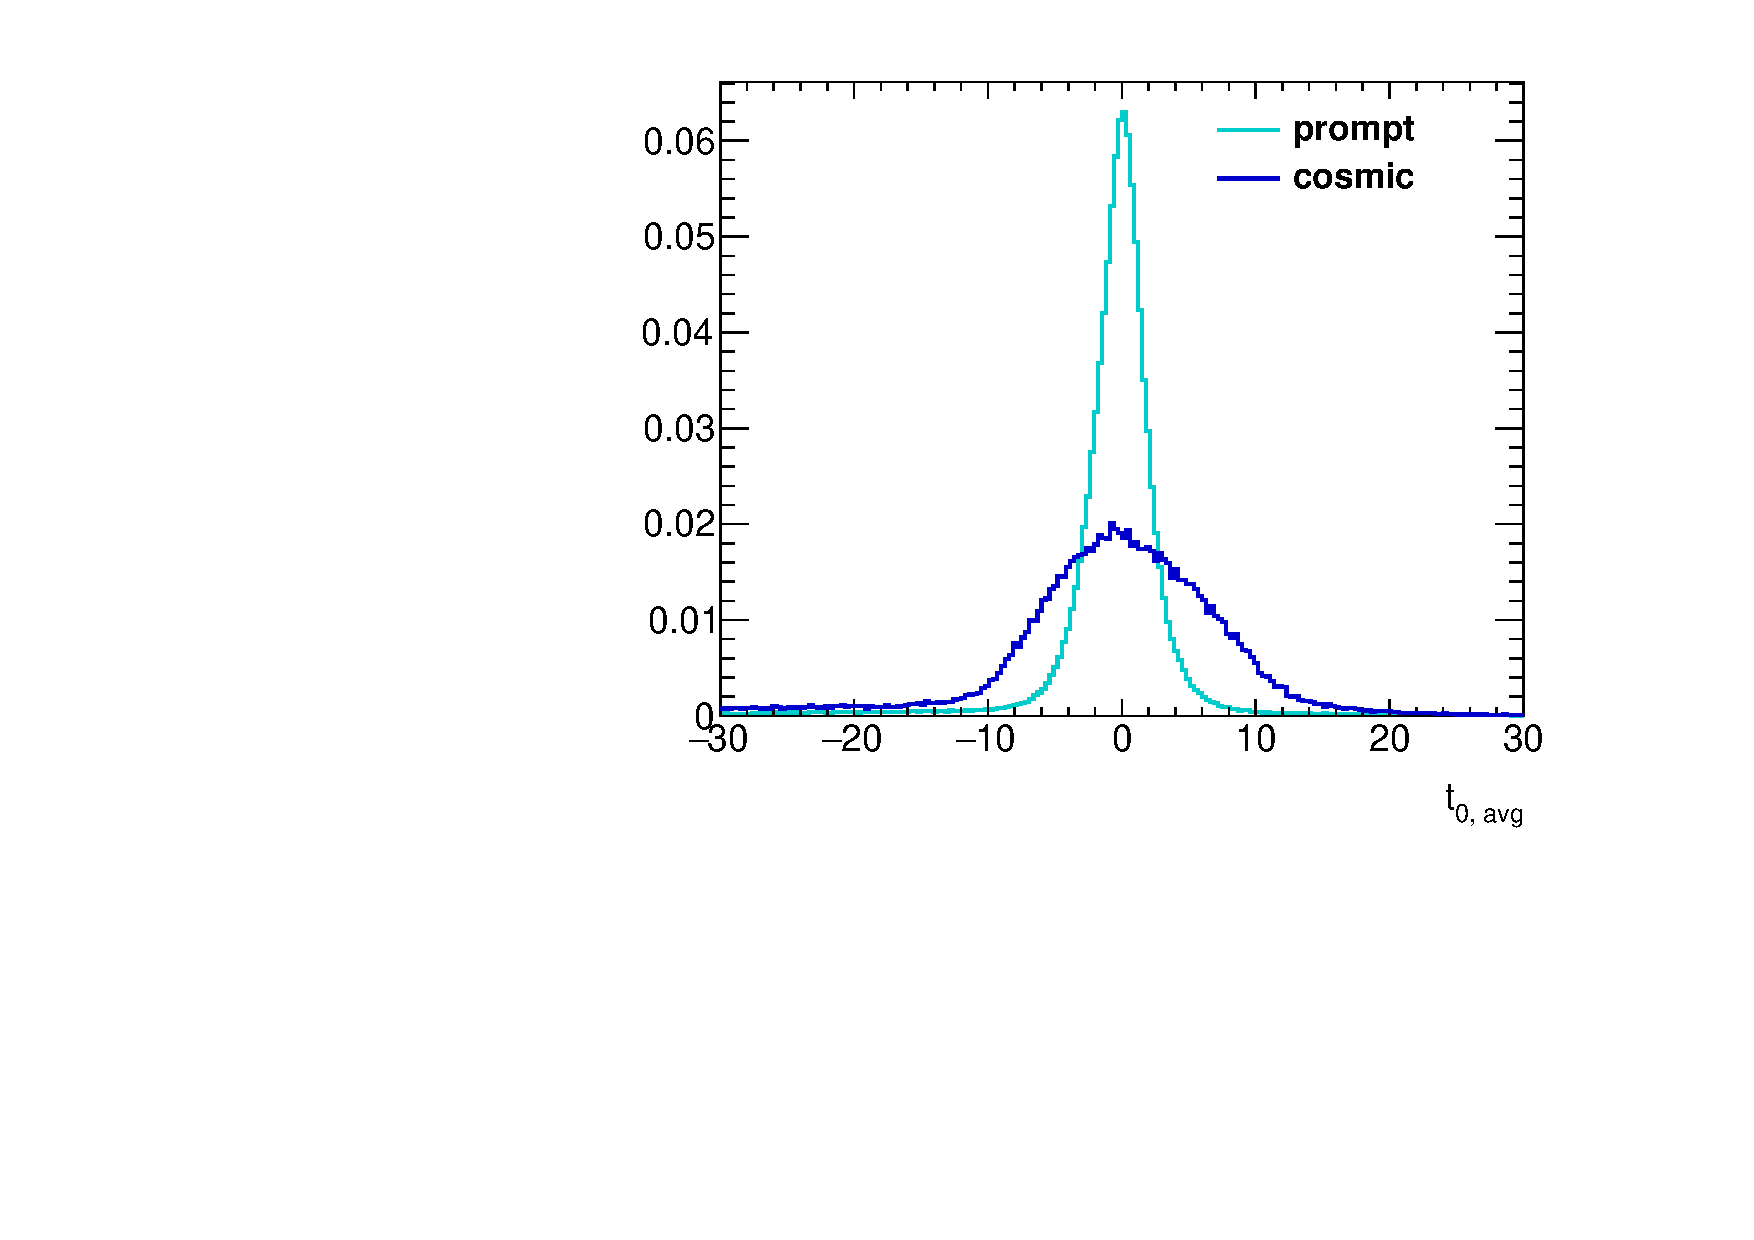
\includegraphics[width=0.38\textwidth]{figures/cosmics/t0_avg_template_comp.pdf}
  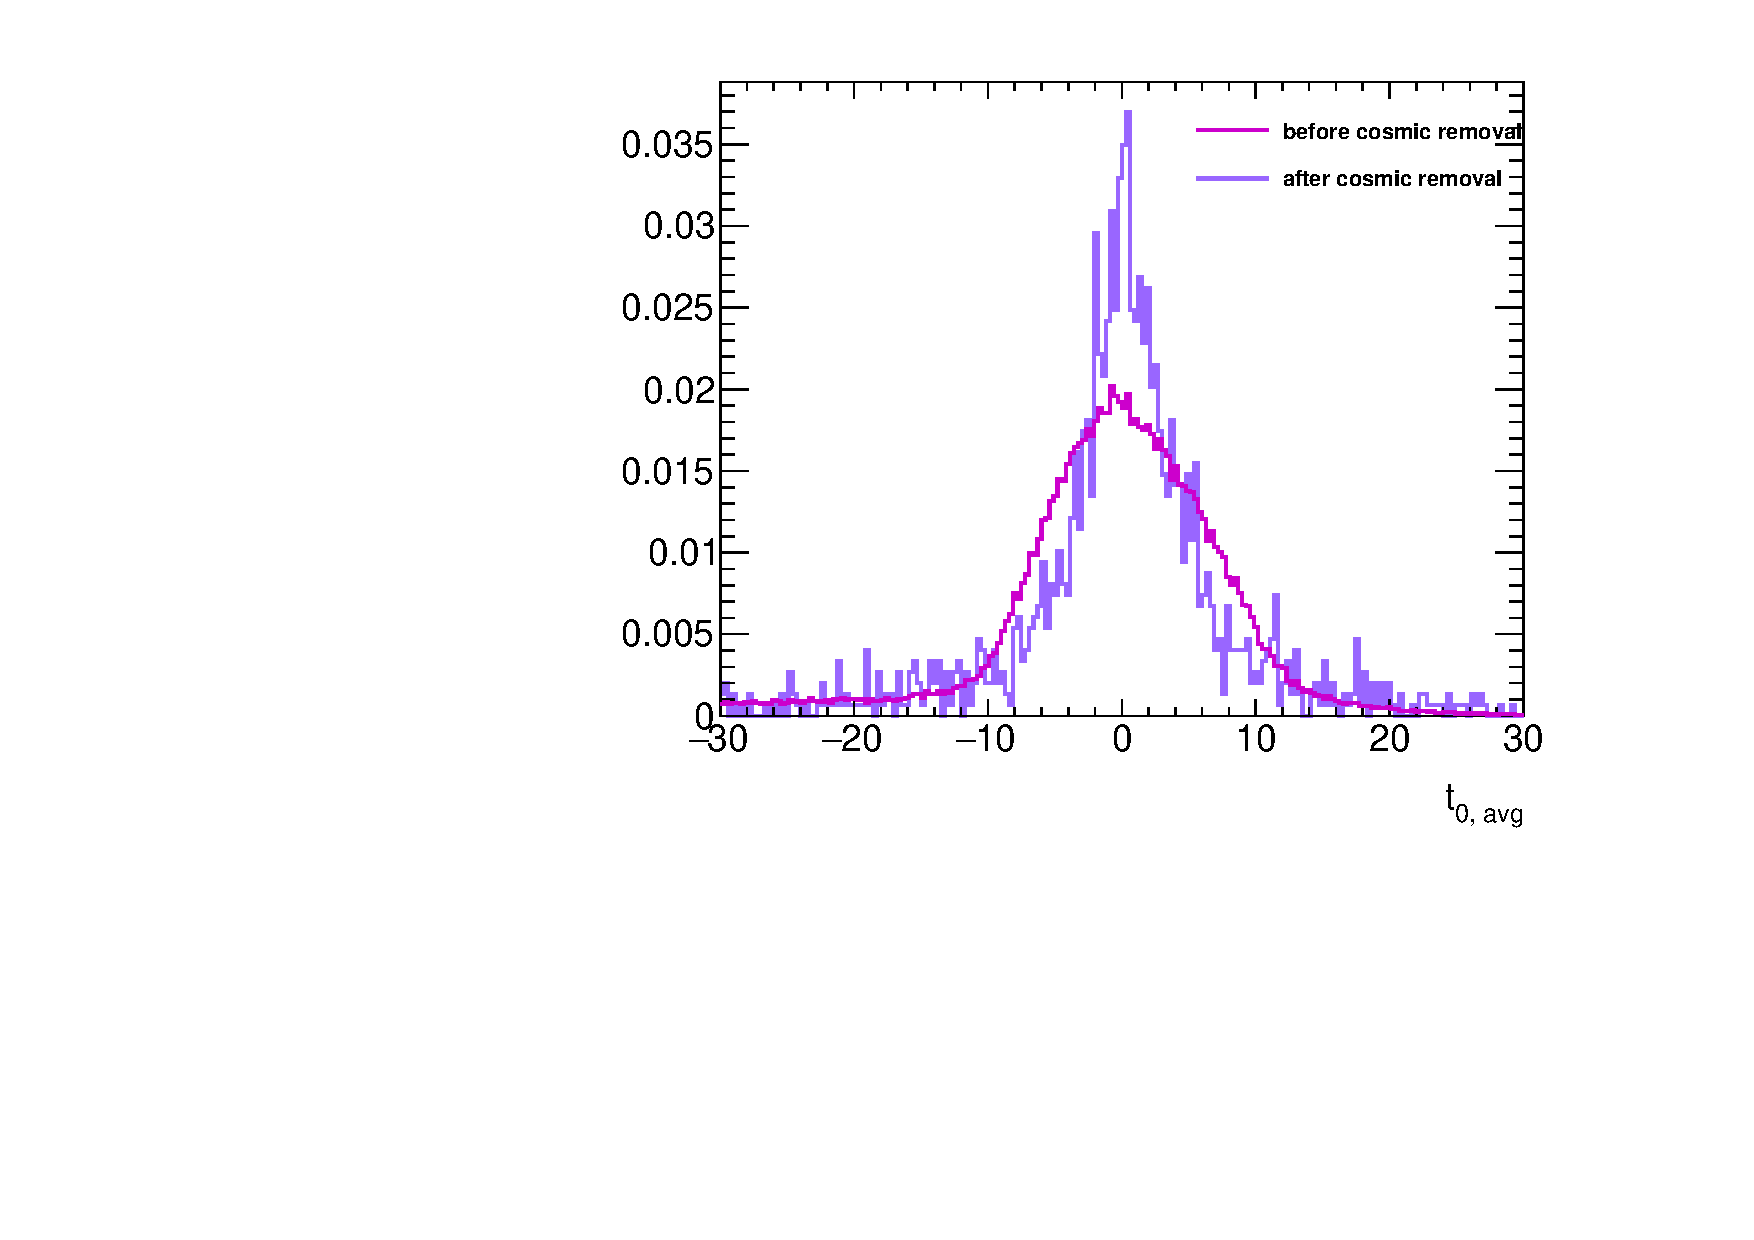
\includegraphics[width=0.38\textwidth]{figures/cosmics/t0_avg_prepost_comp.pdf}
  \caption{\tavg of cosmic and prompt muons used as templates to the fit (left) and VR-$\mu$ dataset before and after removal of cosmic tagged muons on which the fit was performed.}
  \label{fig:d0_t0avg}
\end{figure}


\begin{figure}[!ht]
  \centering
  \begin{subfigure}[b]{0.4\textwidth}
 	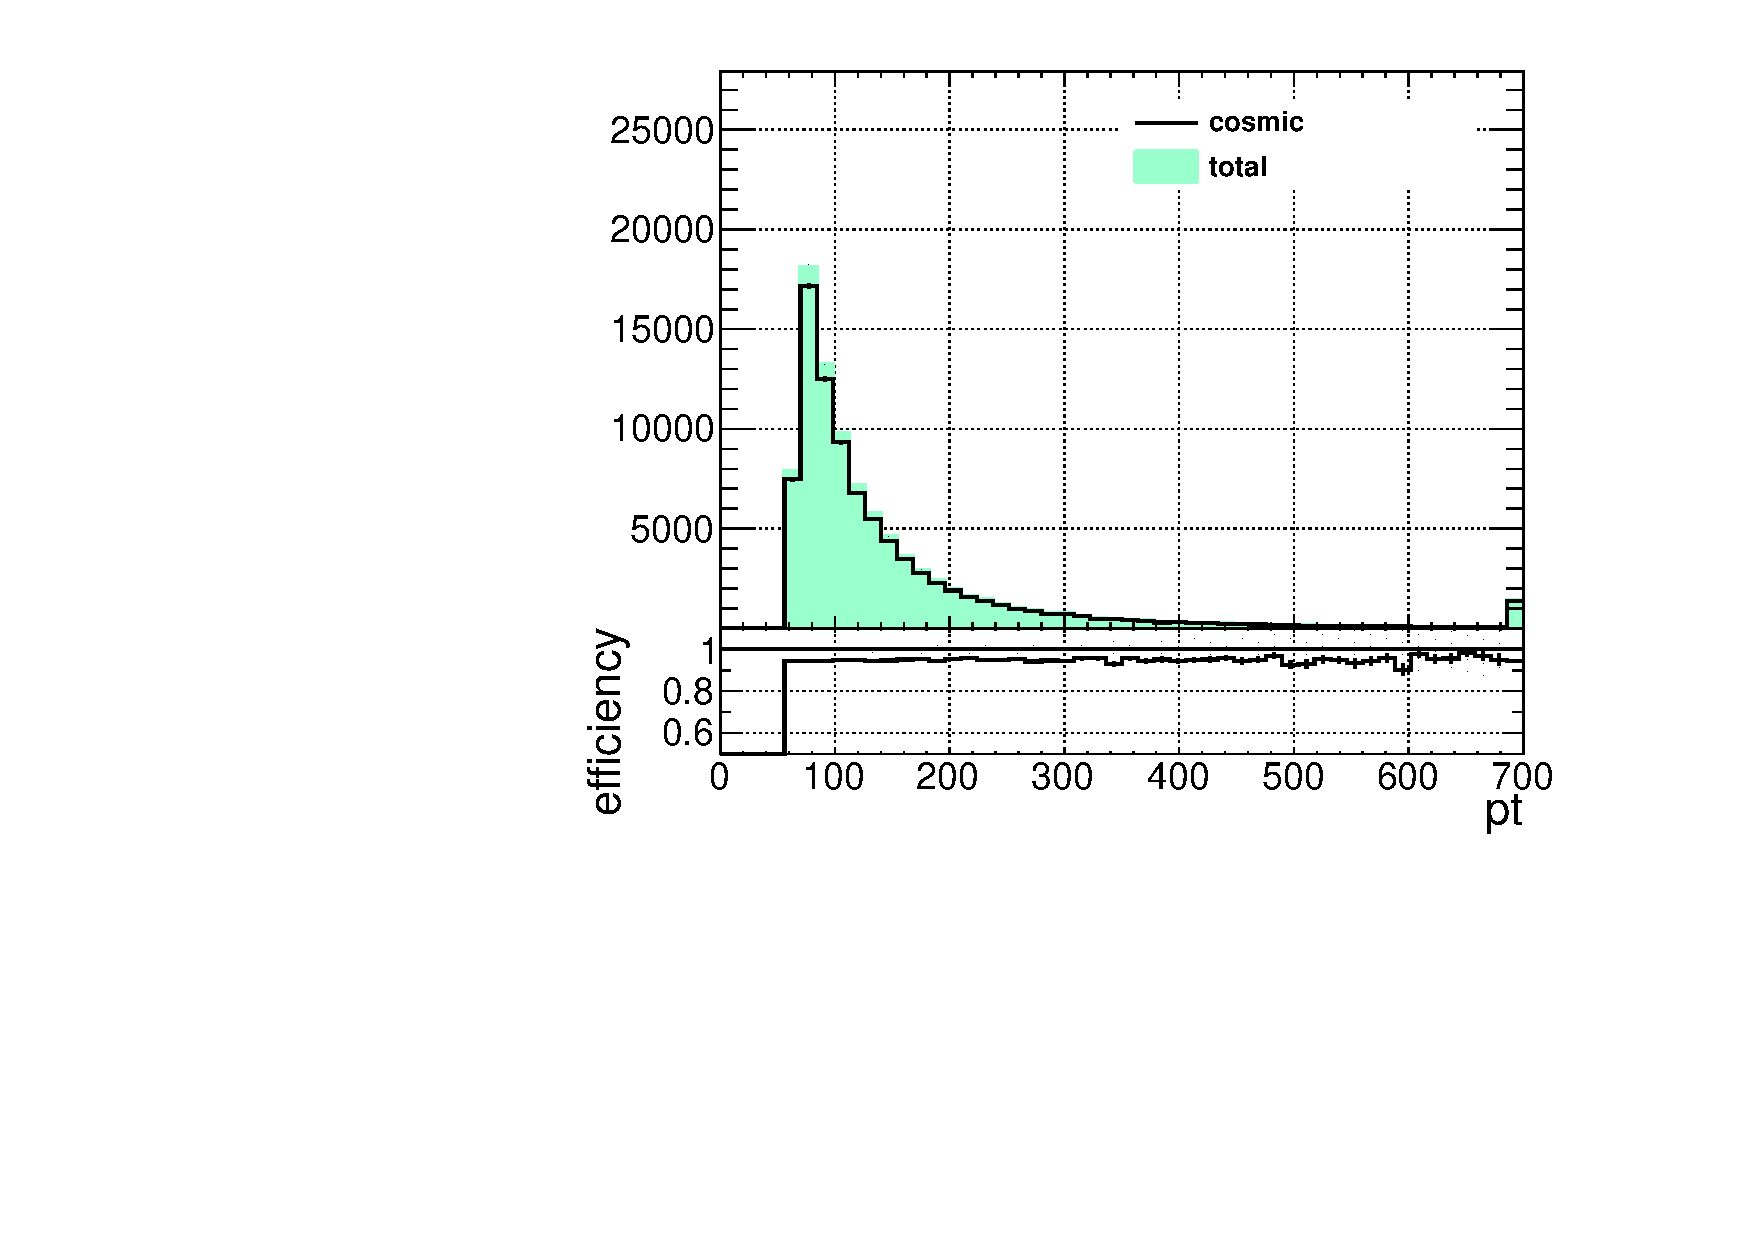
\includegraphics[width=\textwidth]{figures/cosmics/wider_tag_ratio_pt.pdf}
  	\caption{VR-$\mu$ data with respect to \pt}
  \end{subfigure}
  \begin{subfigure}[b]{0.4\textwidth}
 	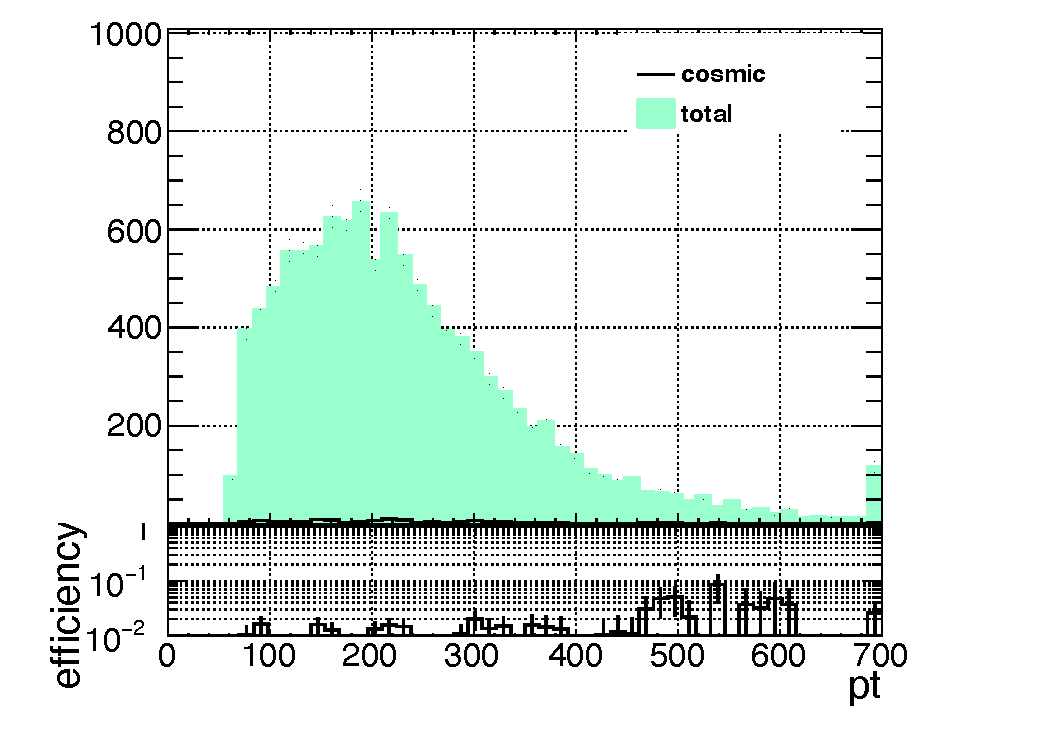
\includegraphics[width=\textwidth]{figures/cosmics/mc_300_ratio_pt.pdf}
  	\caption{Signal \ac{MC} with respect to \pt}
  \end{subfigure}

  \begin{subfigure}[b]{0.4\textwidth}
  	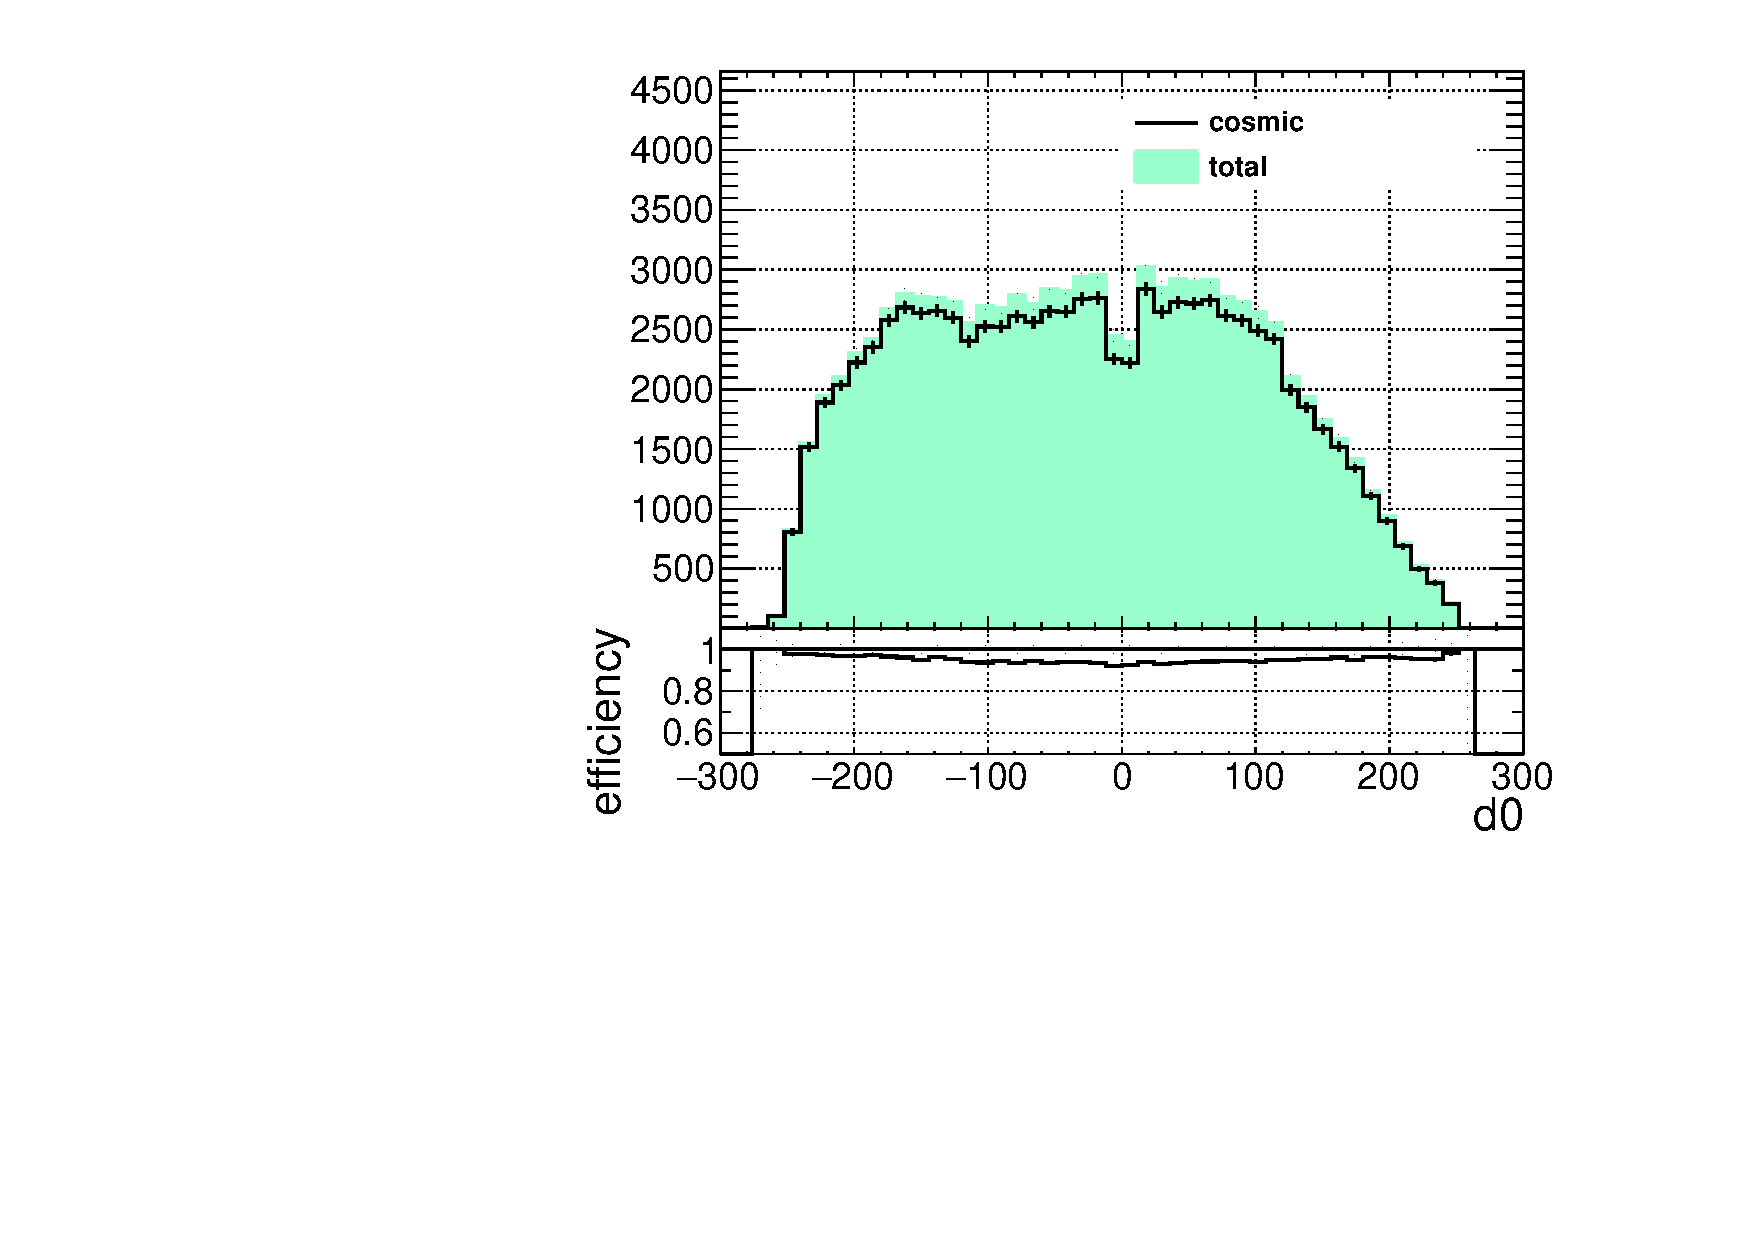
\includegraphics[width=\textwidth]{figures/cosmics/wider_tag_ratio_d0.pdf}
  	\caption{VR-$\mu$ data with respect to \dz}
  \end{subfigure}
  \begin{subfigure}[b]{0.4\textwidth}
  	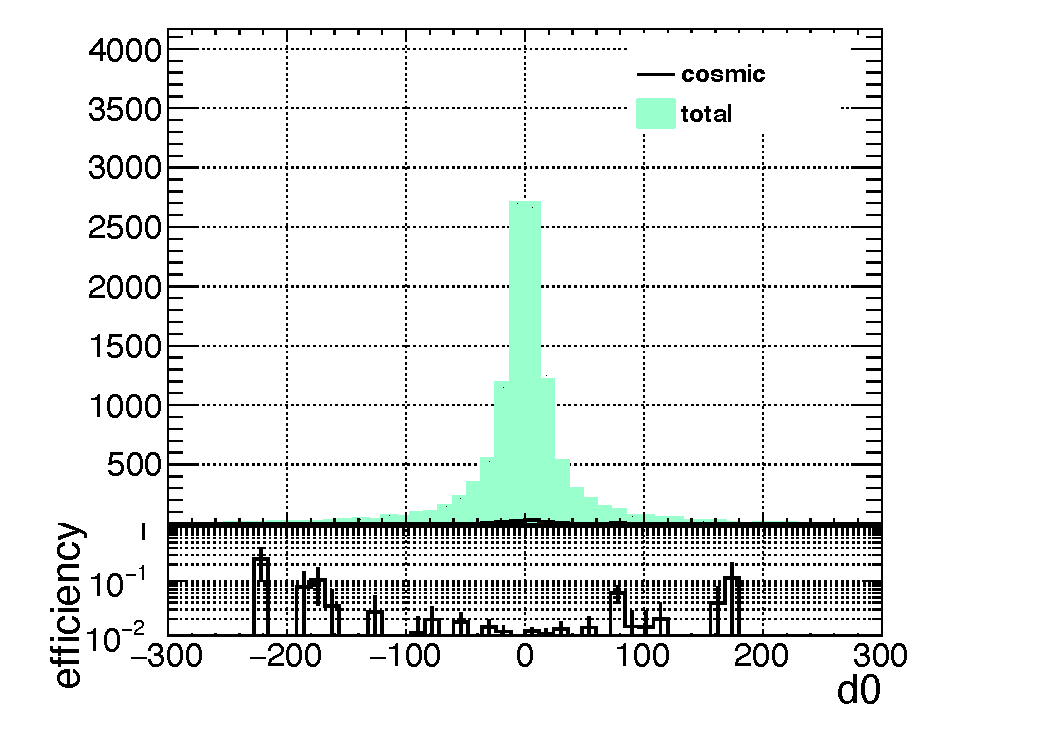
\includegraphics[width=\textwidth]{figures/cosmics/mc_300_ratio_d0.pdf}
  	\caption{Signal \ac{MC} with respect to \dz}
  \end{subfigure}

  \begin{subfigure}[b]{0.4\textwidth}
  	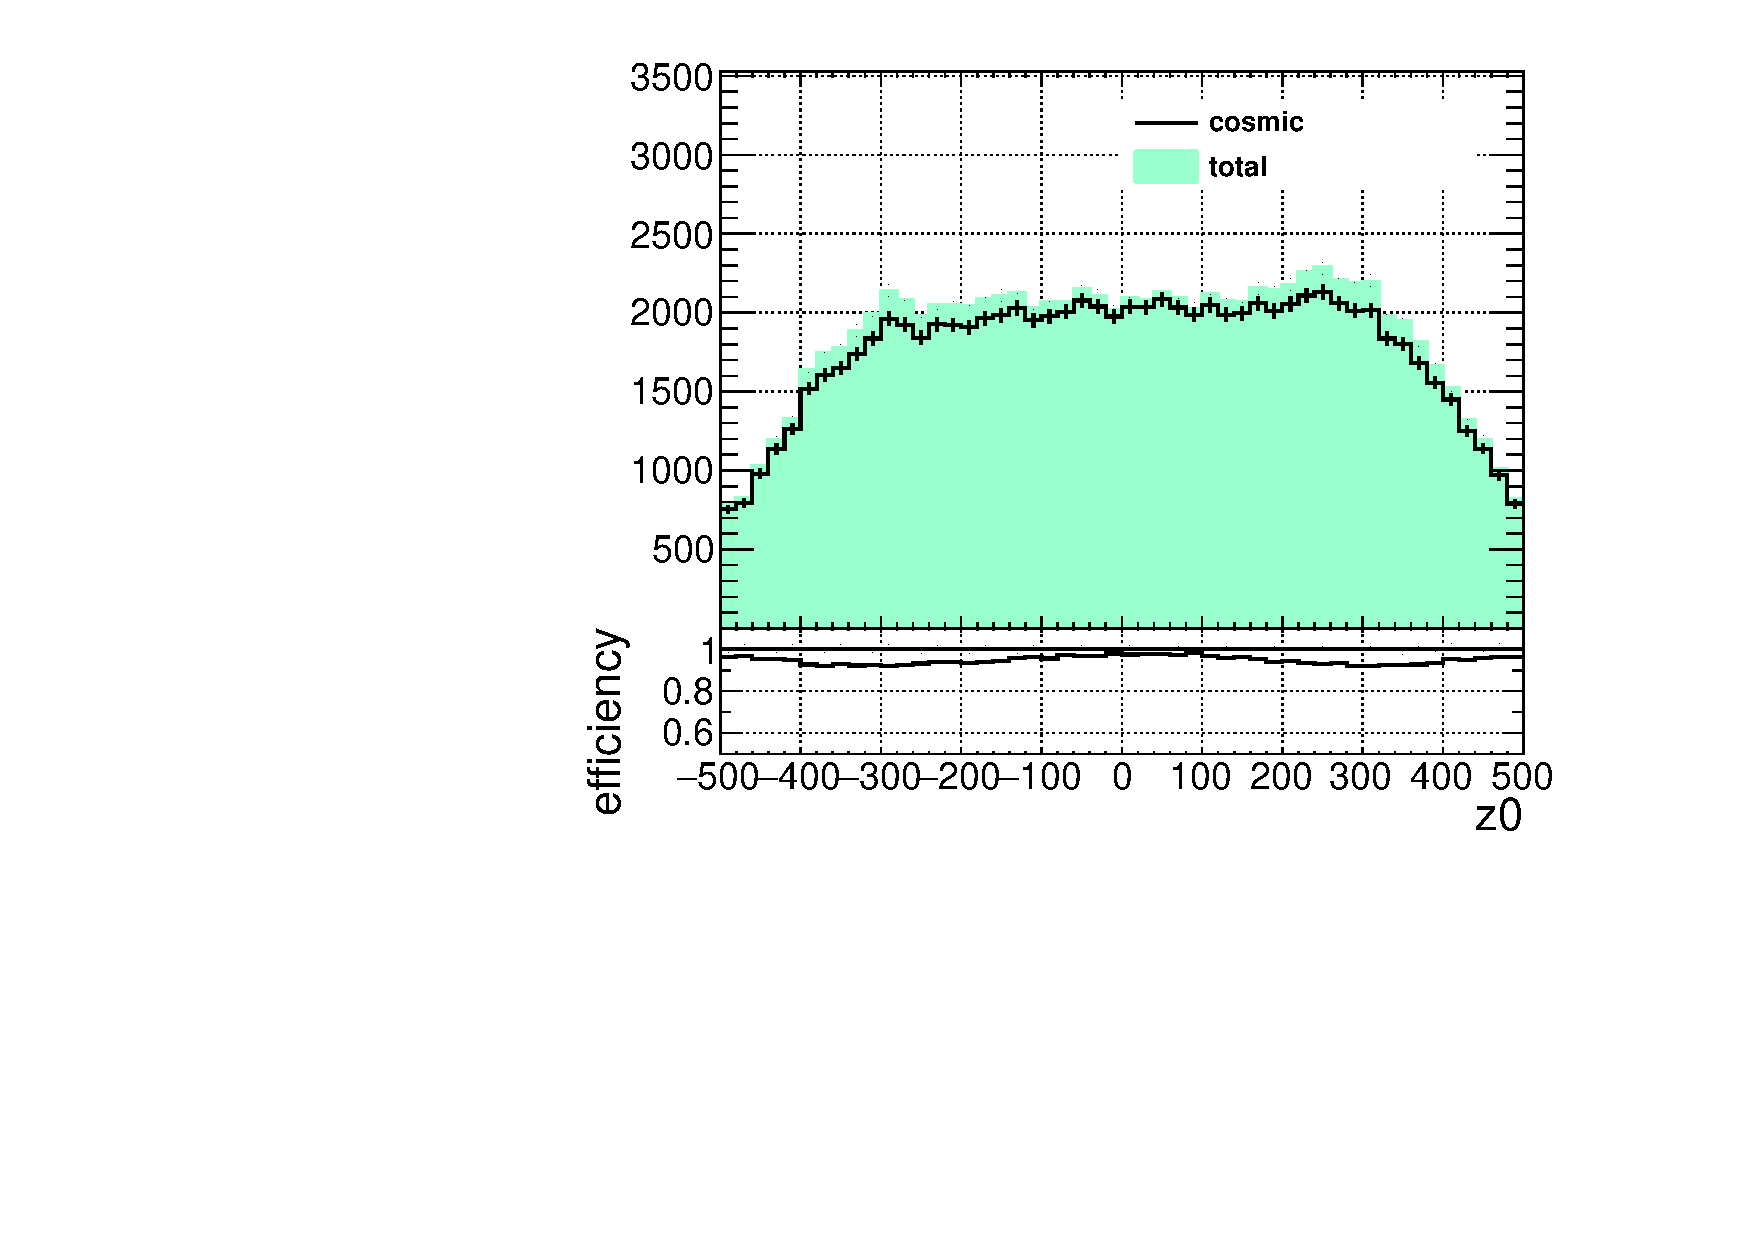
\includegraphics[width=\textwidth]{figures/cosmics/wider_tag_ratio_z0.pdf}
  	\caption{VR-$\mu$ data with respect to \z}
  \end{subfigure}
  \begin{subfigure}[b]{0.4\textwidth}
  	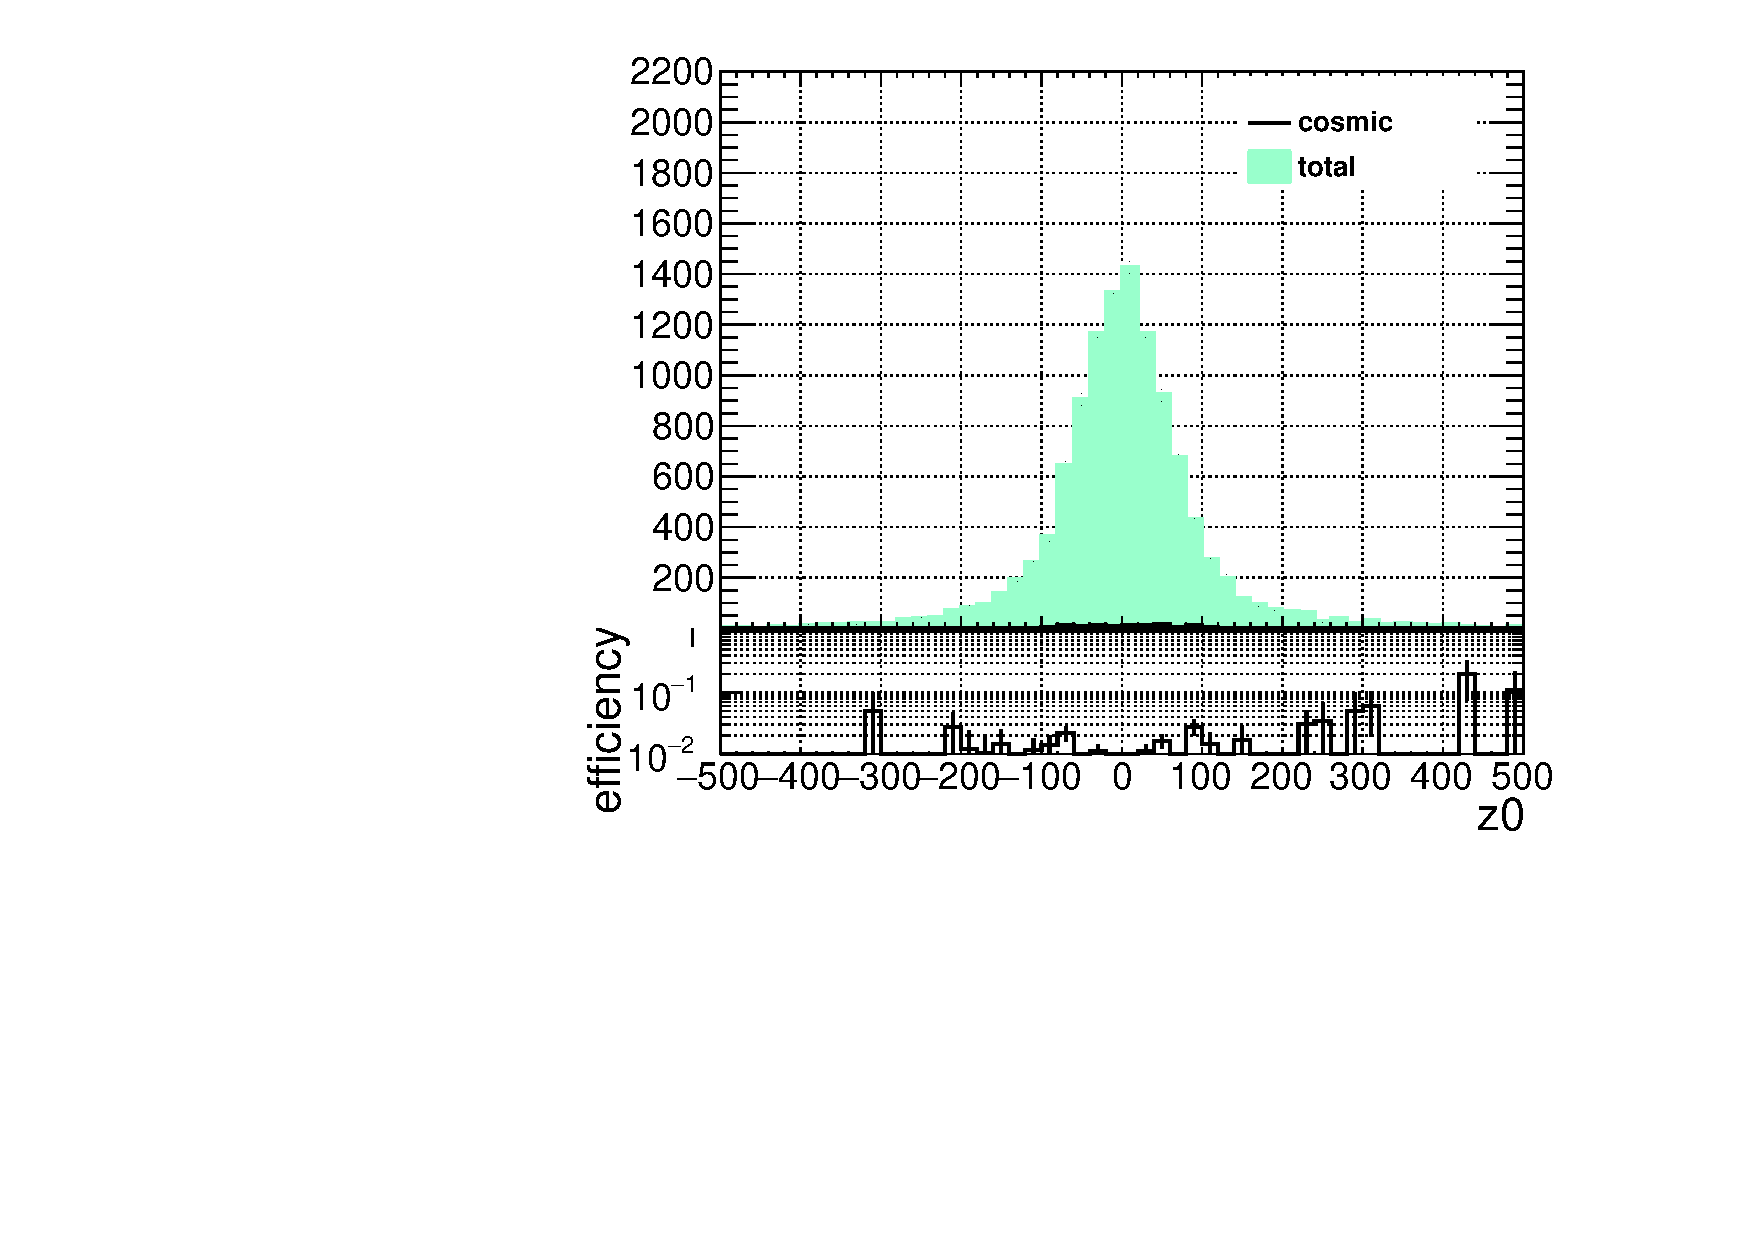
\includegraphics[width=\textwidth]{figures/cosmics/mc_300_ratio_z0.pdf}
  	\caption{Signal \ac{MC} with respect to \z}
  \end{subfigure}
  \caption{Cosmic tagging efficiency with respect to kinematic variables in VR-$\mu$ data and signal \ac{MC}}
\end{figure}
\begin{figure}[!ht]
  \ContinuedFloat
  \centering
  \begin{subfigure}[b]{0.4\textwidth}
  	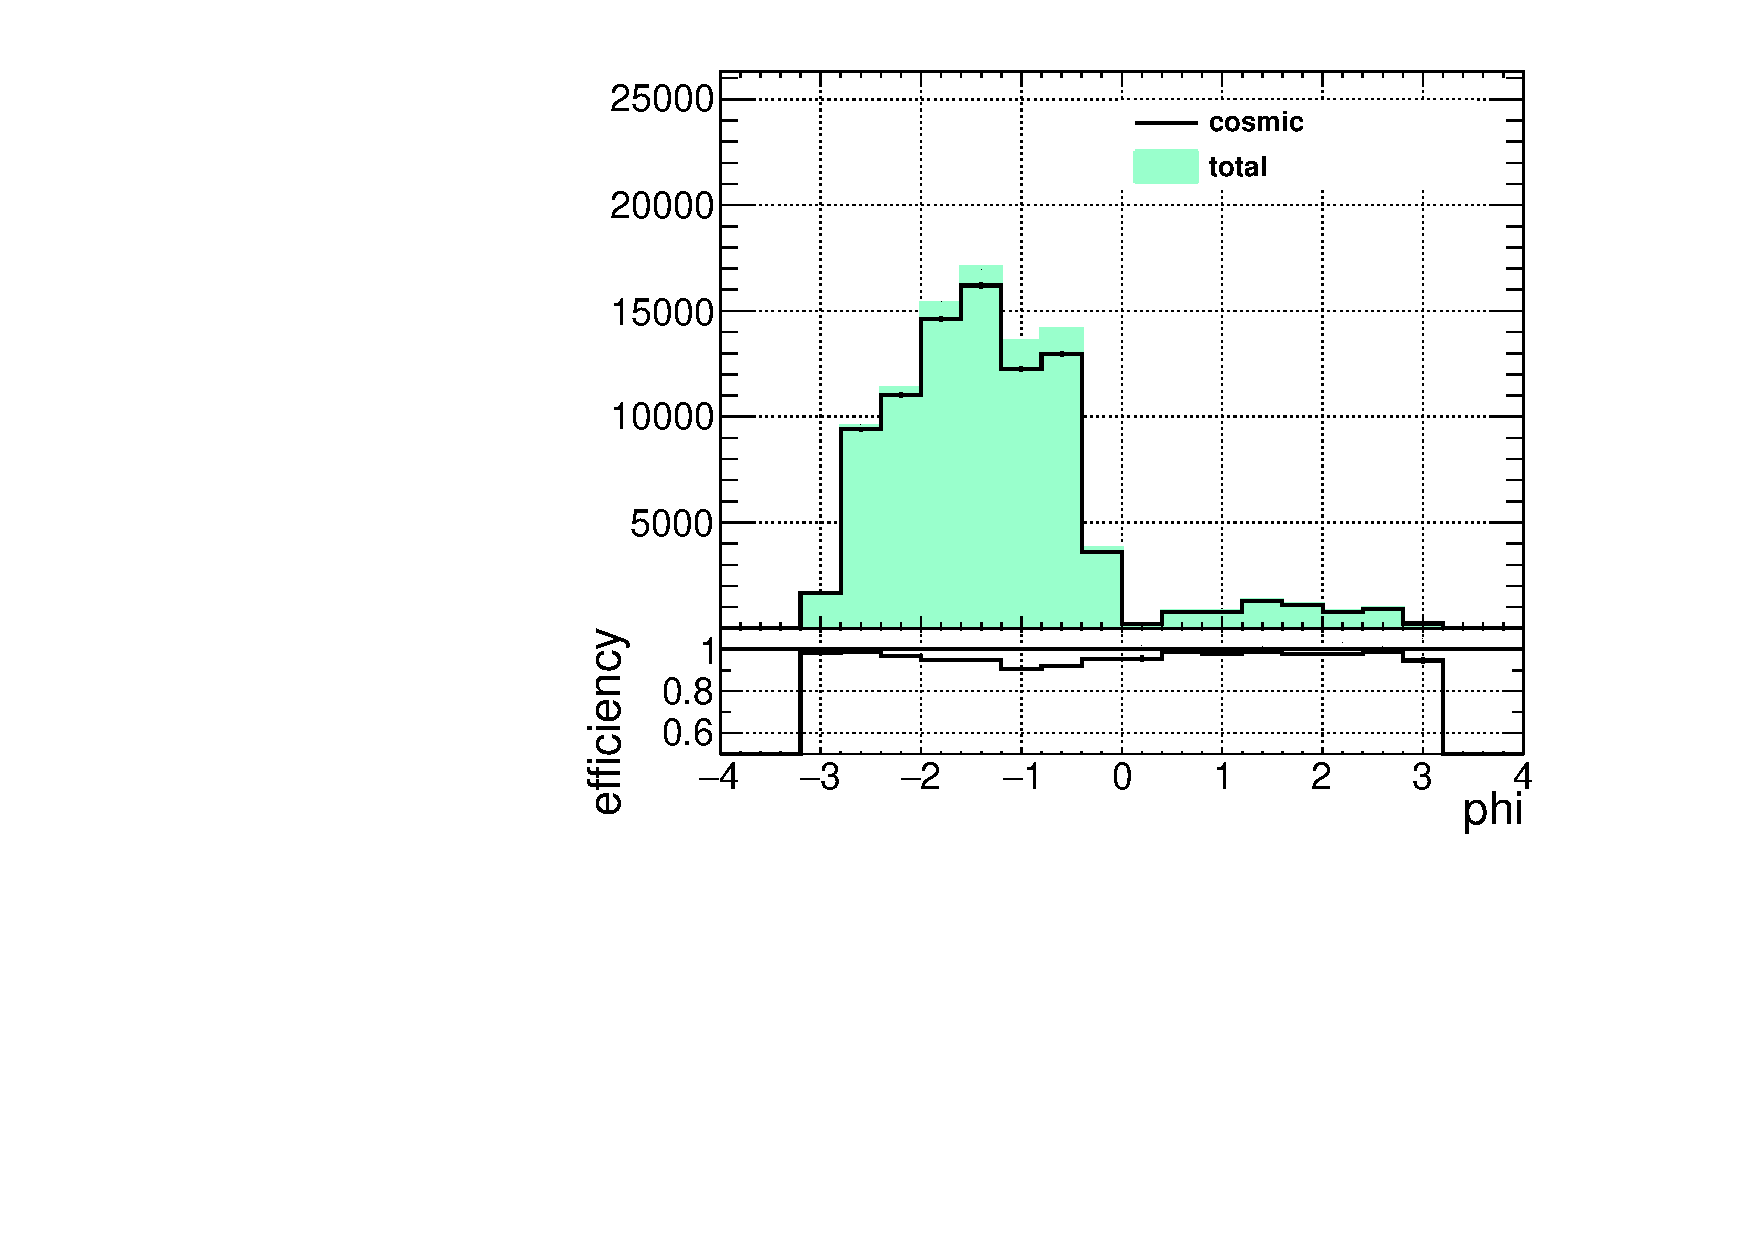
\includegraphics[width=\textwidth]{figures/cosmics/wider_tag_ratio_phi.pdf}
  	\caption{VR-$\mu$ data with respect to $\phi$}
  \end{subfigure}
  \begin{subfigure}[b]{0.4\textwidth}
 	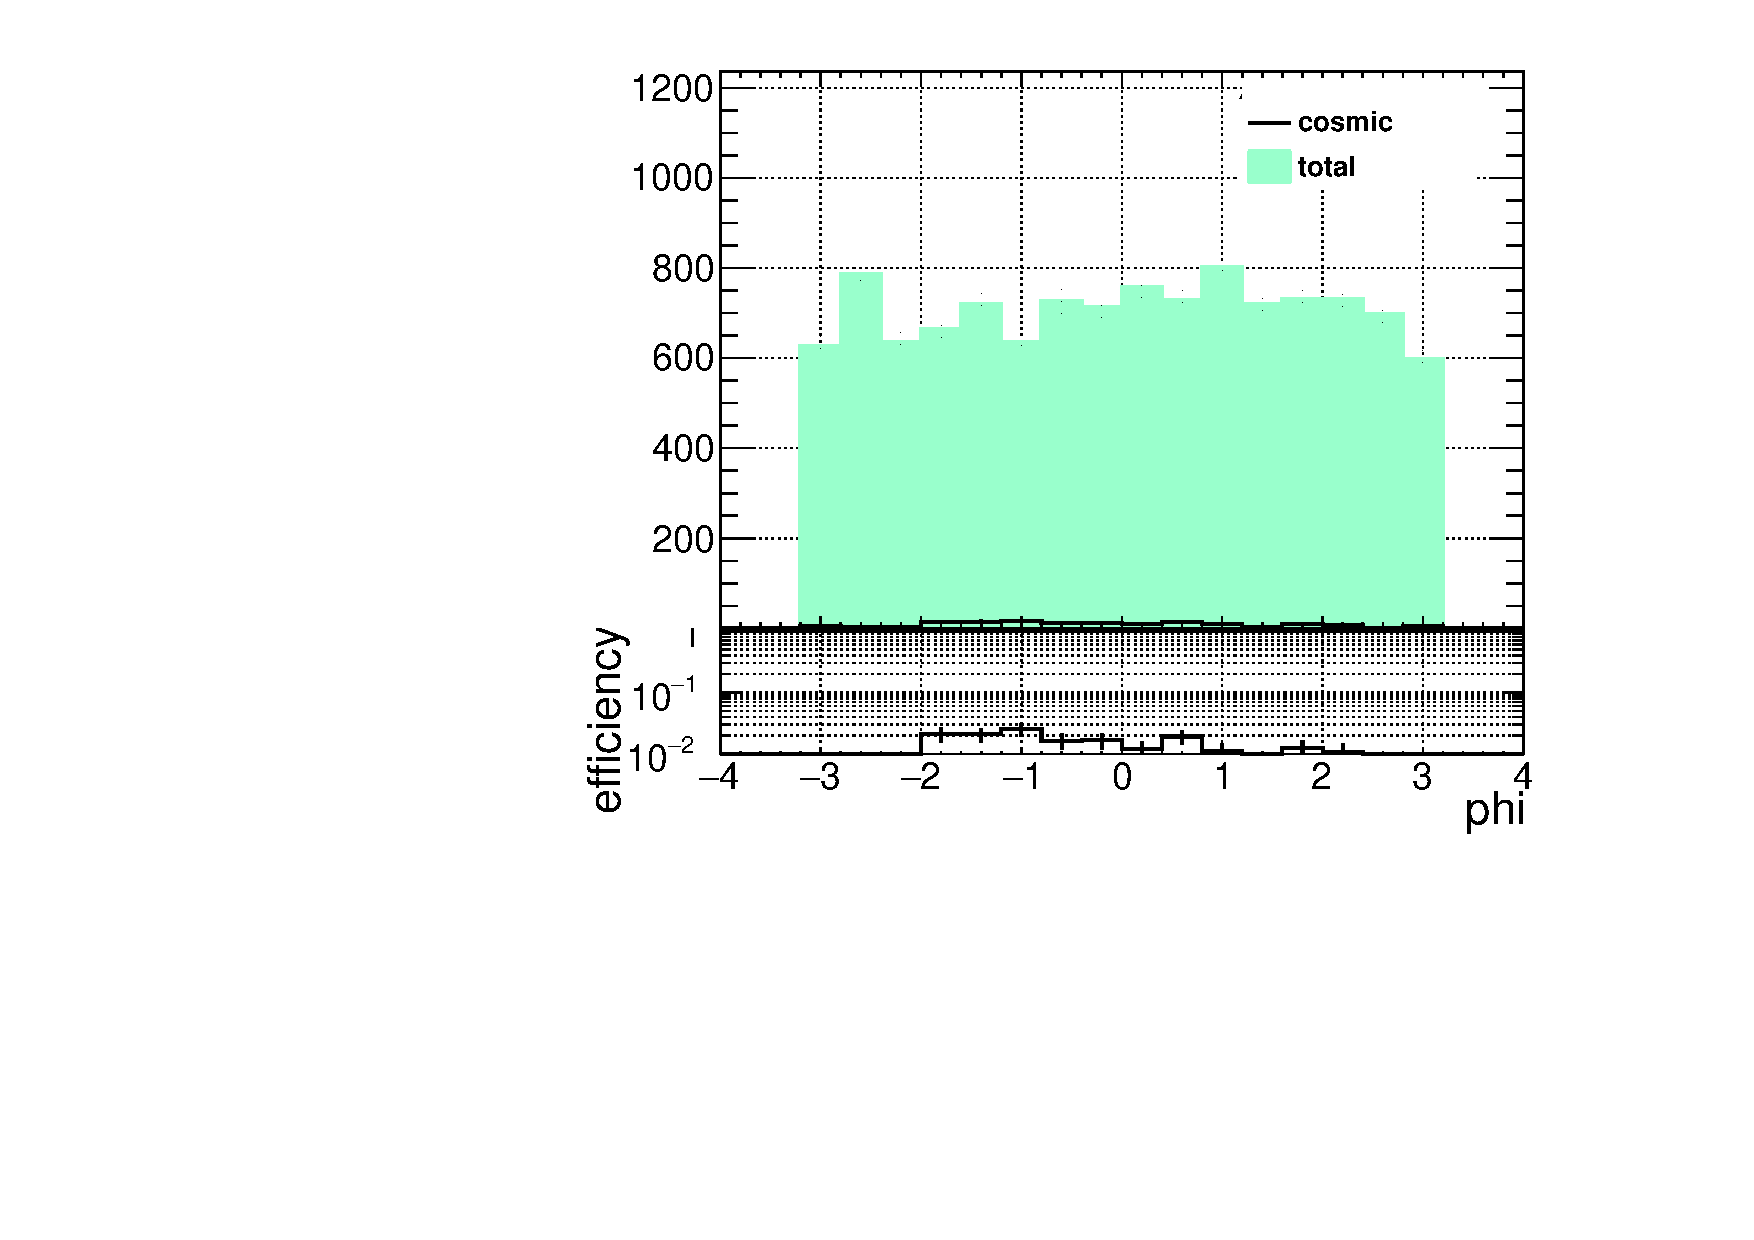
\includegraphics[width=\textwidth]{figures/cosmics/mc_300_ratio_phi.pdf}
  	\caption{Signal \ac{MC} with respect to $\phi$}
  \end{subfigure}

 \begin{subfigure}[b]{0.4\textwidth}
  	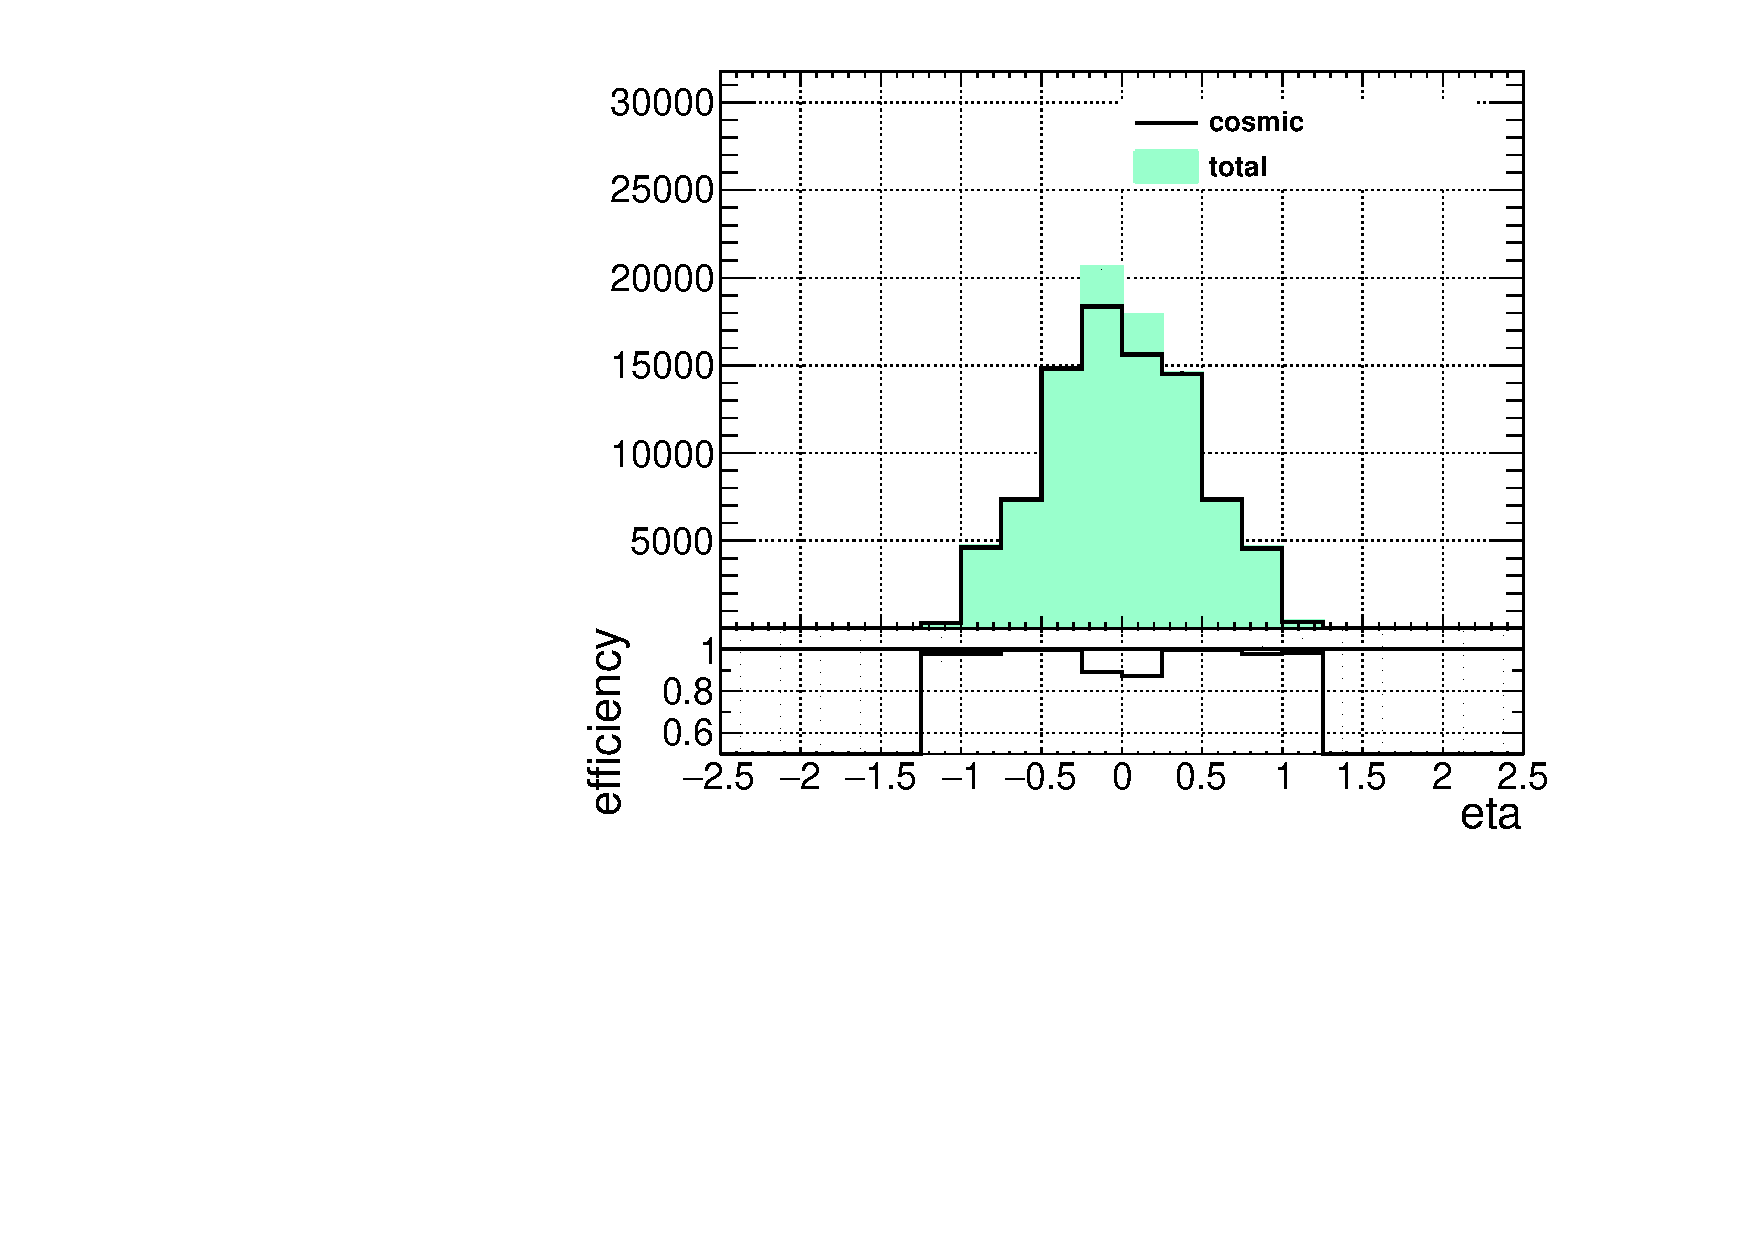
\includegraphics[width=\textwidth]{figures/cosmics/wider_tag_ratio_eta.pdf}
  	\caption{VR-$\mu$ data with respect to $\eta$}
  \end{subfigure}
  \begin{subfigure}[b]{0.4\textwidth}
  	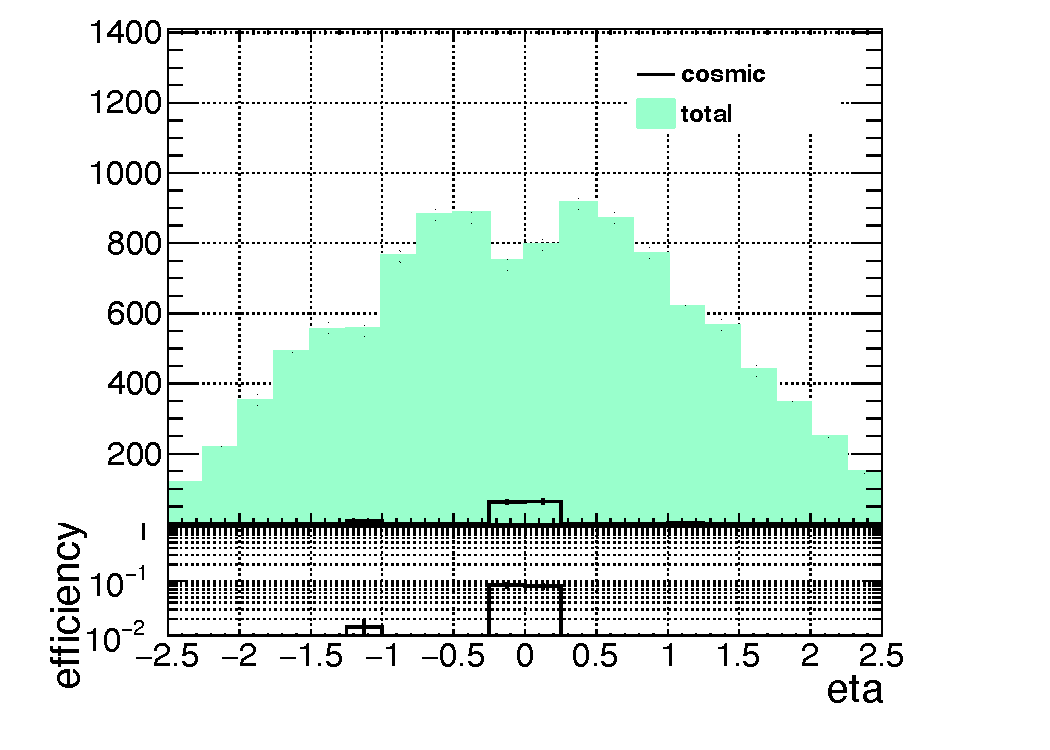
\includegraphics[width=\textwidth]{figures/cosmics/mc_300_ratio_eta.pdf}
  	\caption{Signal \ac{MC} with respect to $\eta$}
  \end{subfigure}
    \caption{Cosmic tagging efficiency with respect to kinematic variables in VR-$\mu$ data and signal \ac{MC}}
  \label{fig:cos_eff}
\end{figure}



%\begin{sidewaysfigure}[h]
%  \centering
%  \begin{subfigure}[b]{\textwidth}
%  	\centering
%  	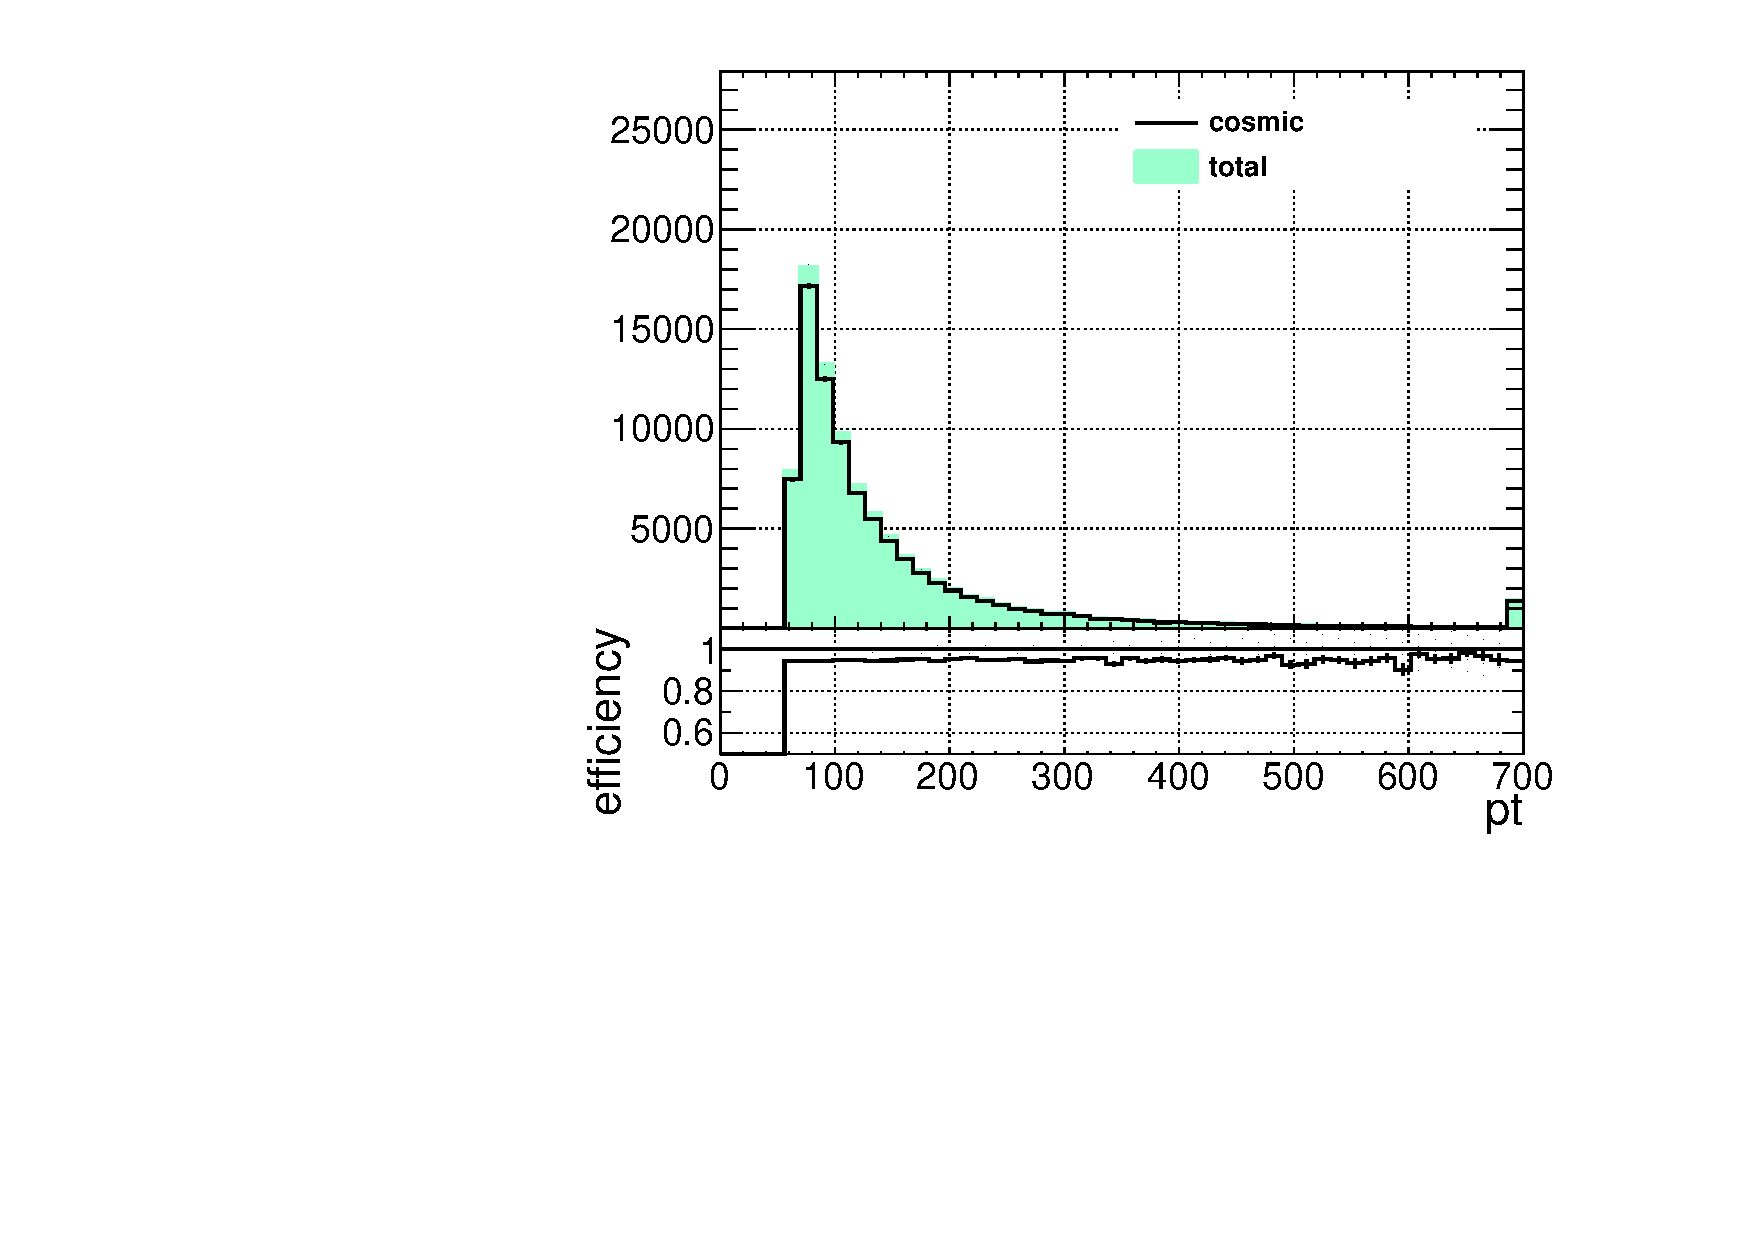
\includegraphics[width=.18\textwidth]{figures/cosmics/wider_tag_ratio_pt.pdf}
%  	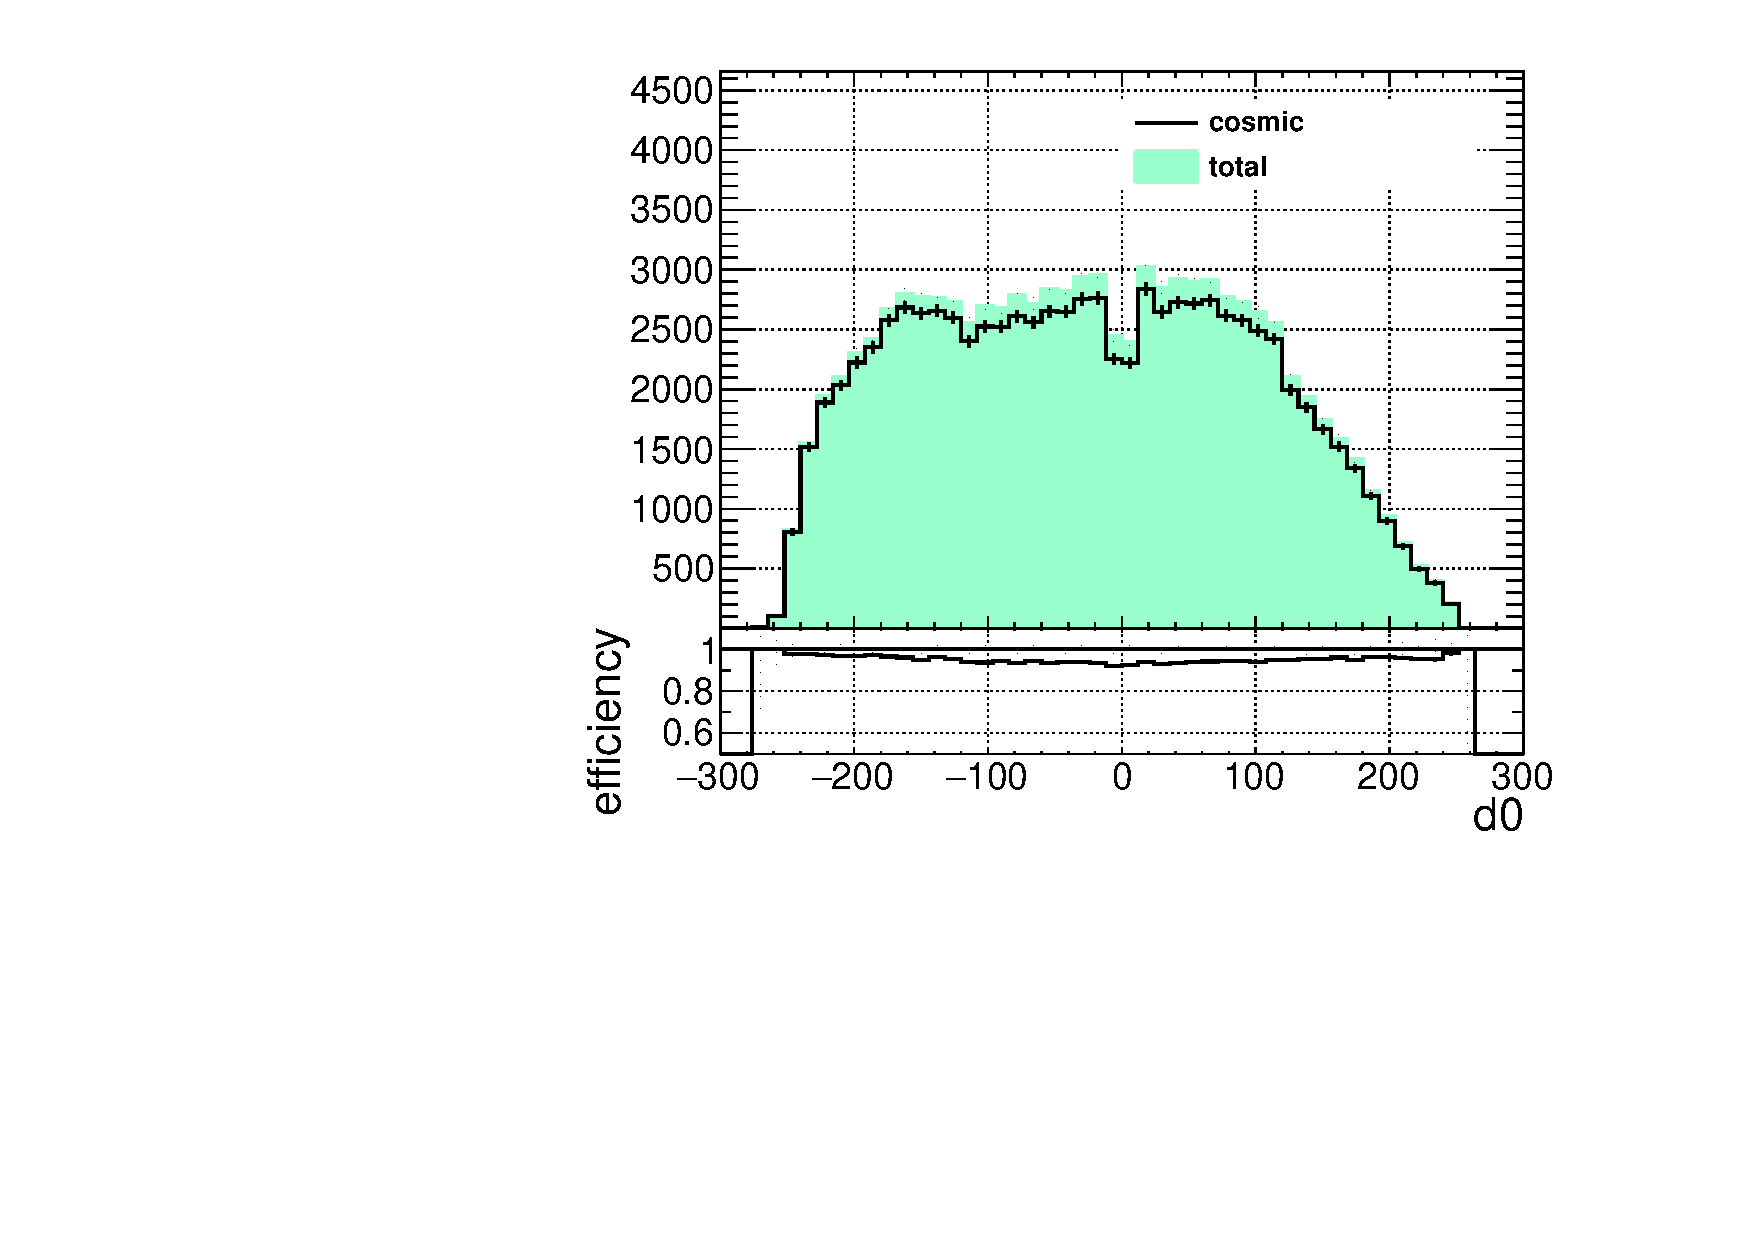
\includegraphics[width=.18\textwidth]{figures/cosmics/wider_tag_ratio_d0.pdf}
% 	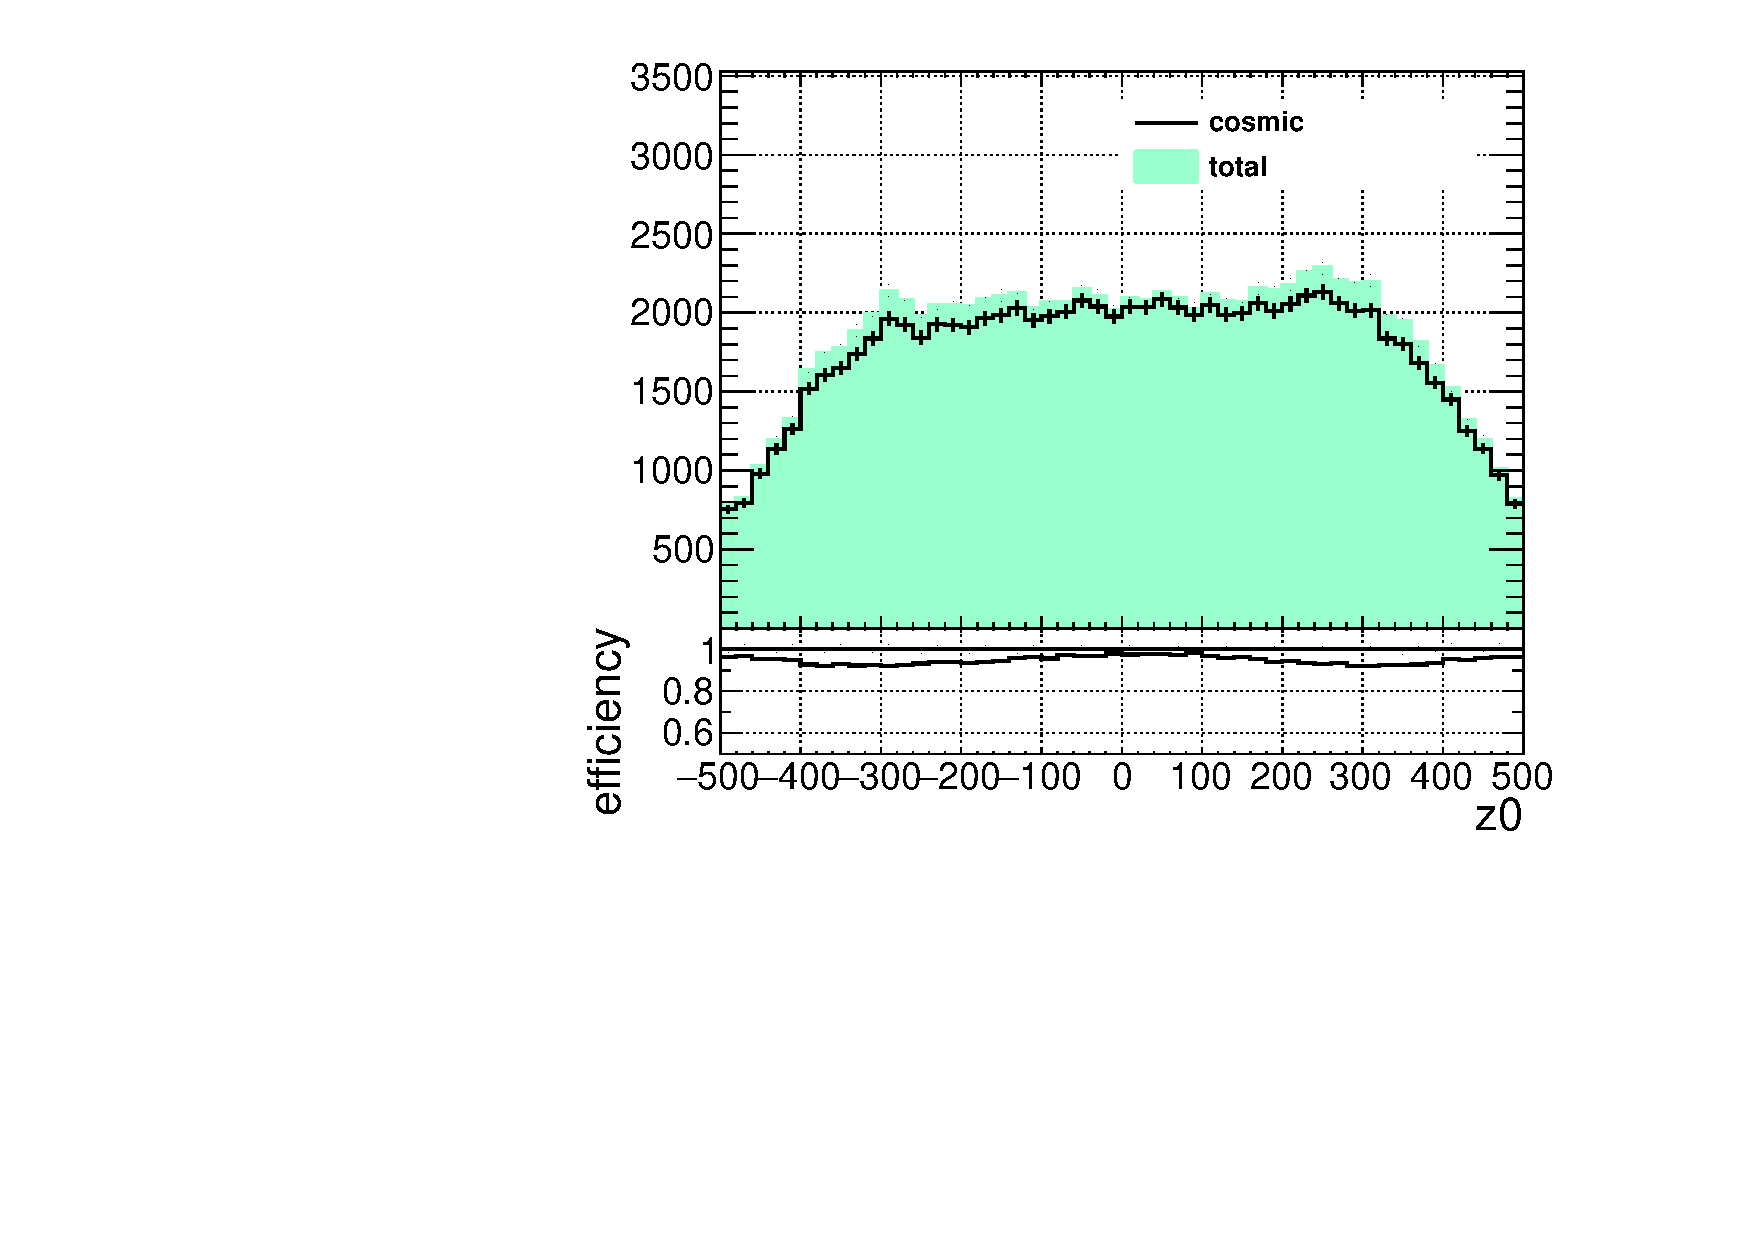
\includegraphics[width=.18\textwidth]{figures/cosmics/wider_tag_ratio_z0.pdf}
% 	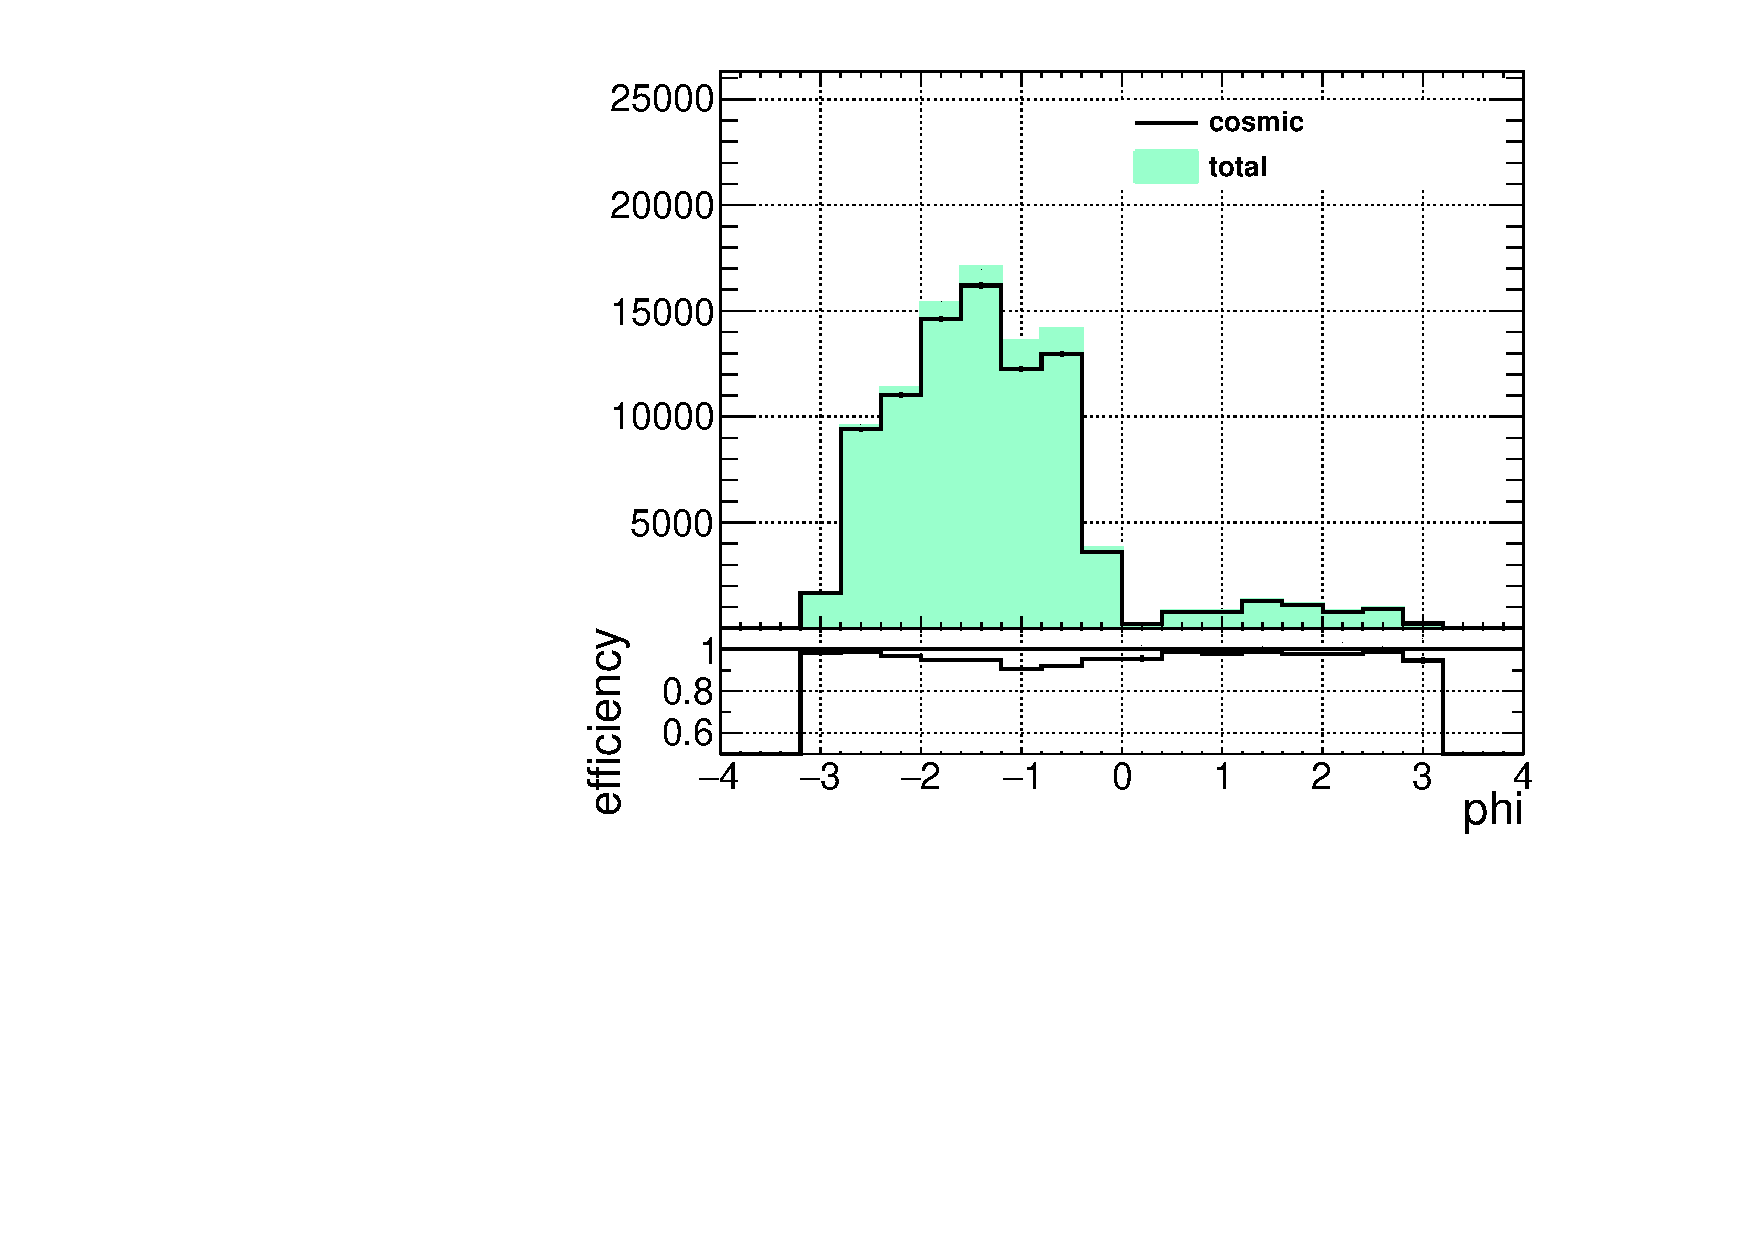
\includegraphics[width=.18\textwidth]{figures/cosmics/wider_tag_ratio_phi.pdf}
% 	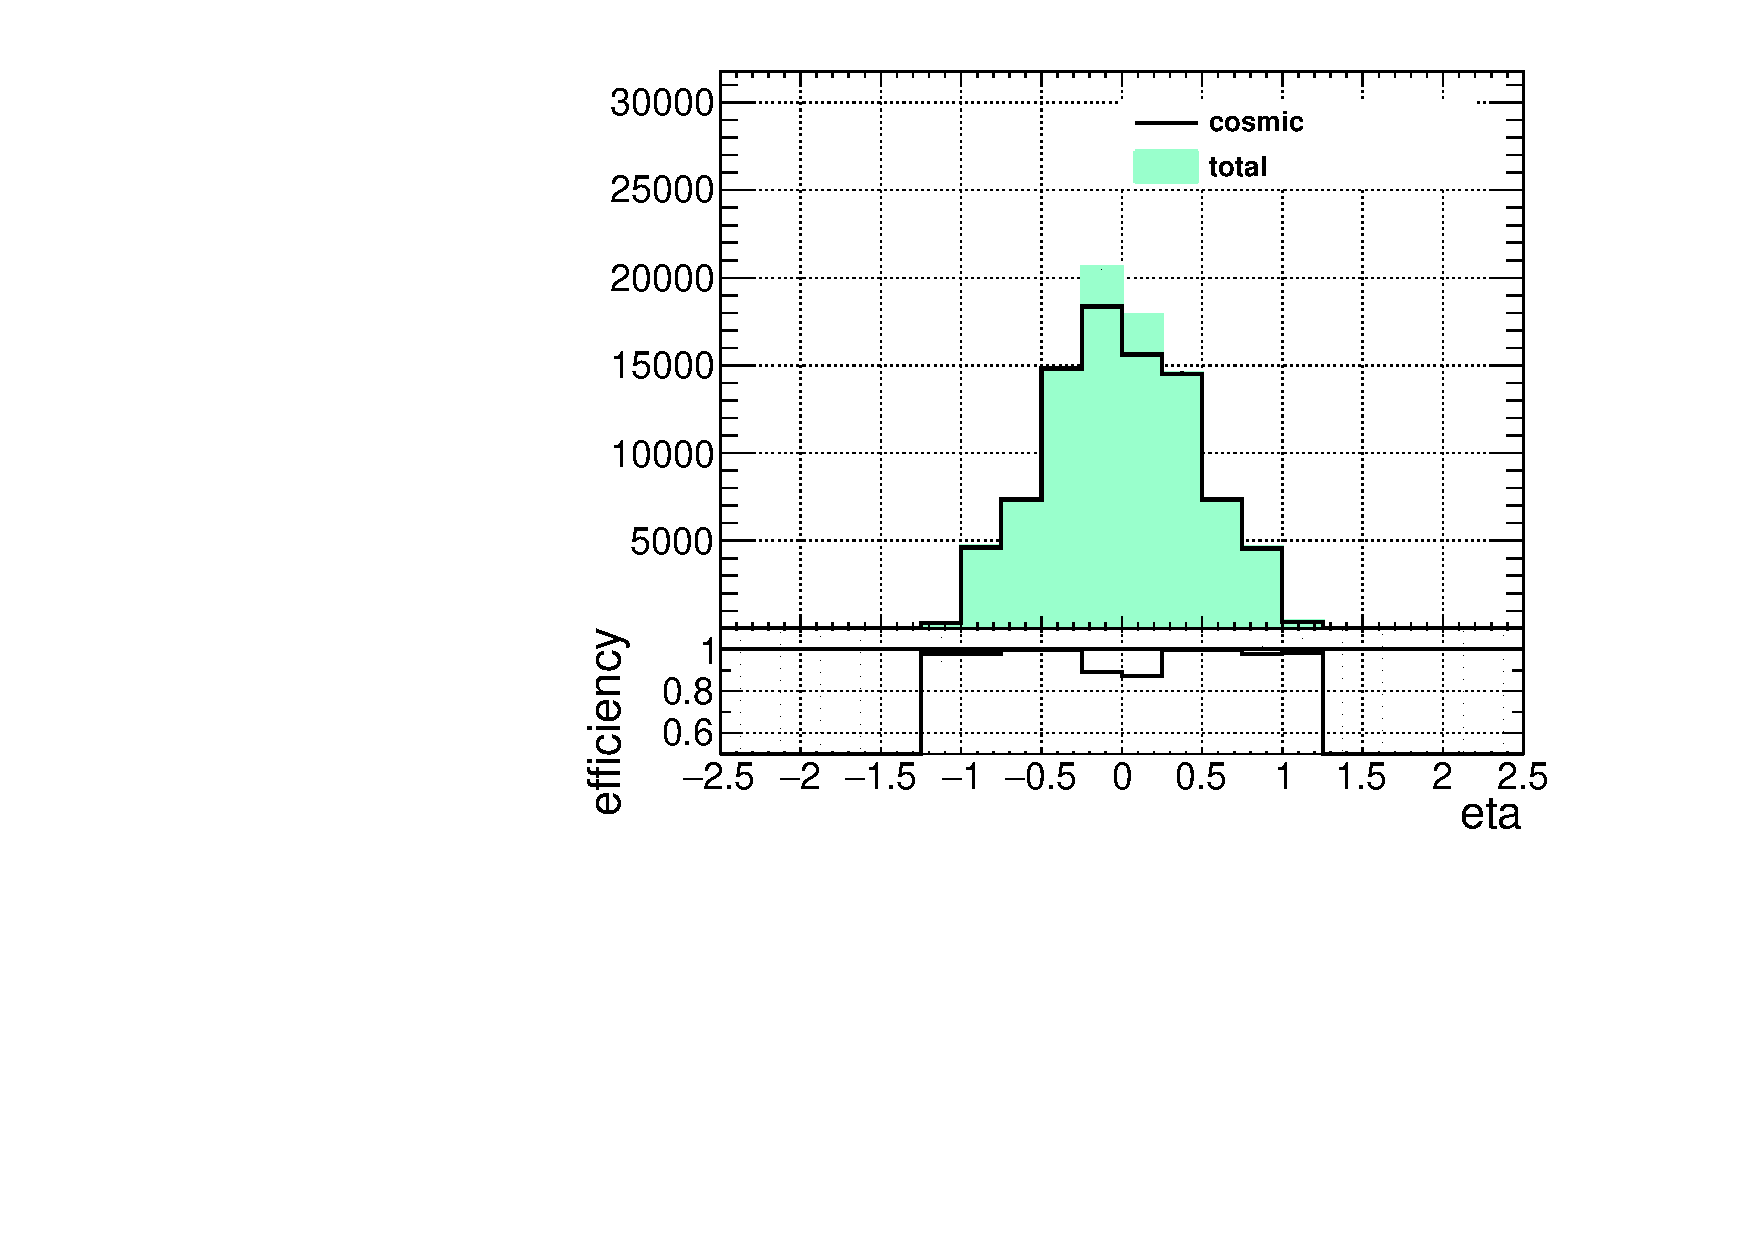
\includegraphics[width=.18\textwidth]{figures/cosmics/wider_tag_ratio_eta.pdf}
% 	\caption{Cosmic tagging efficiency in VR-$\mu$ data}
%  \end{subfigure}

%  \begin{subfigure}[b]{\textwidth}
%  	\centering
%  	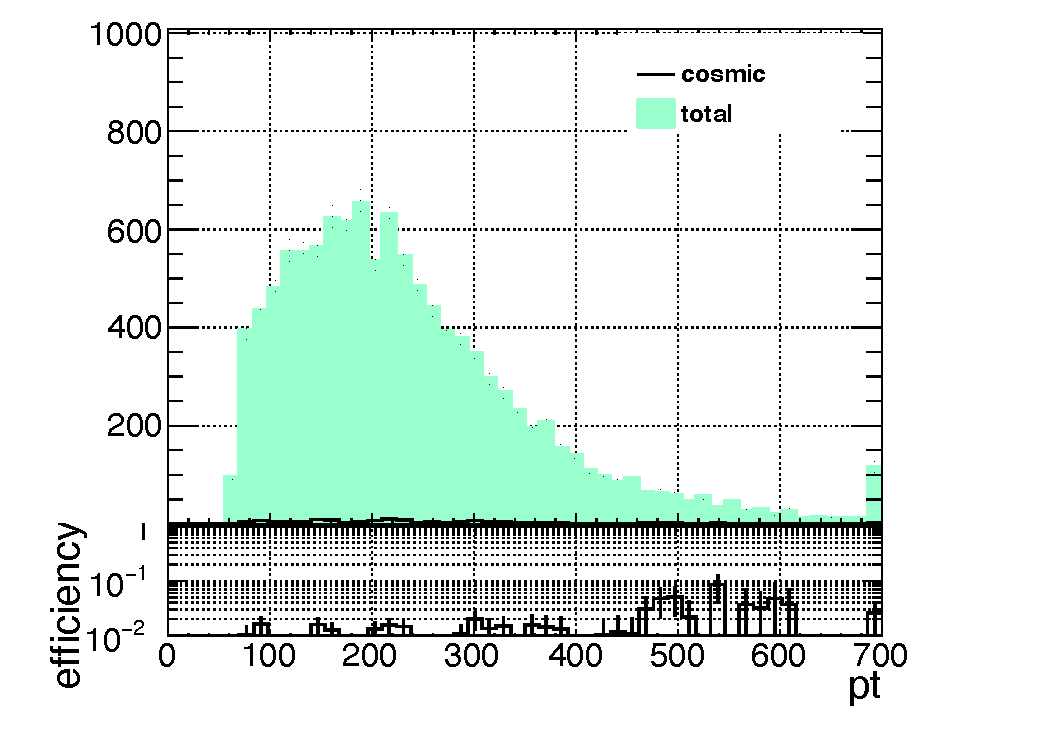
\includegraphics[width=.18\textwidth]{figures/cosmics/mc_300_ratio_pt.pdf}
%  	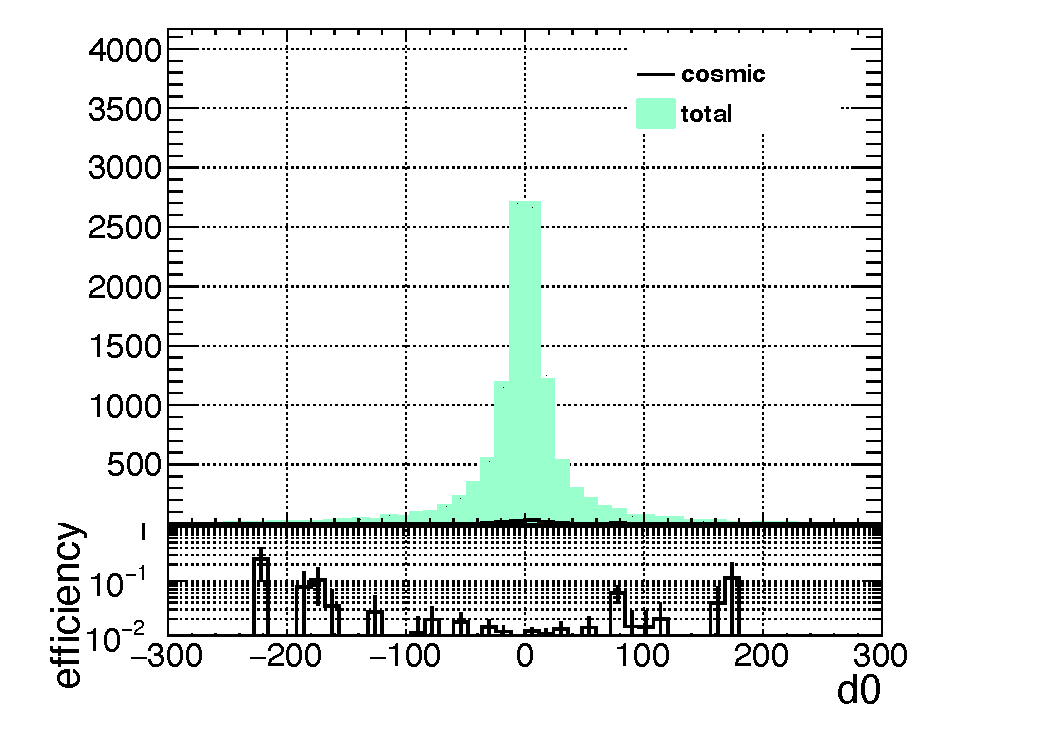
\includegraphics[width=.18\textwidth]{figures/cosmics/mc_300_ratio_d0.pdf}
%  	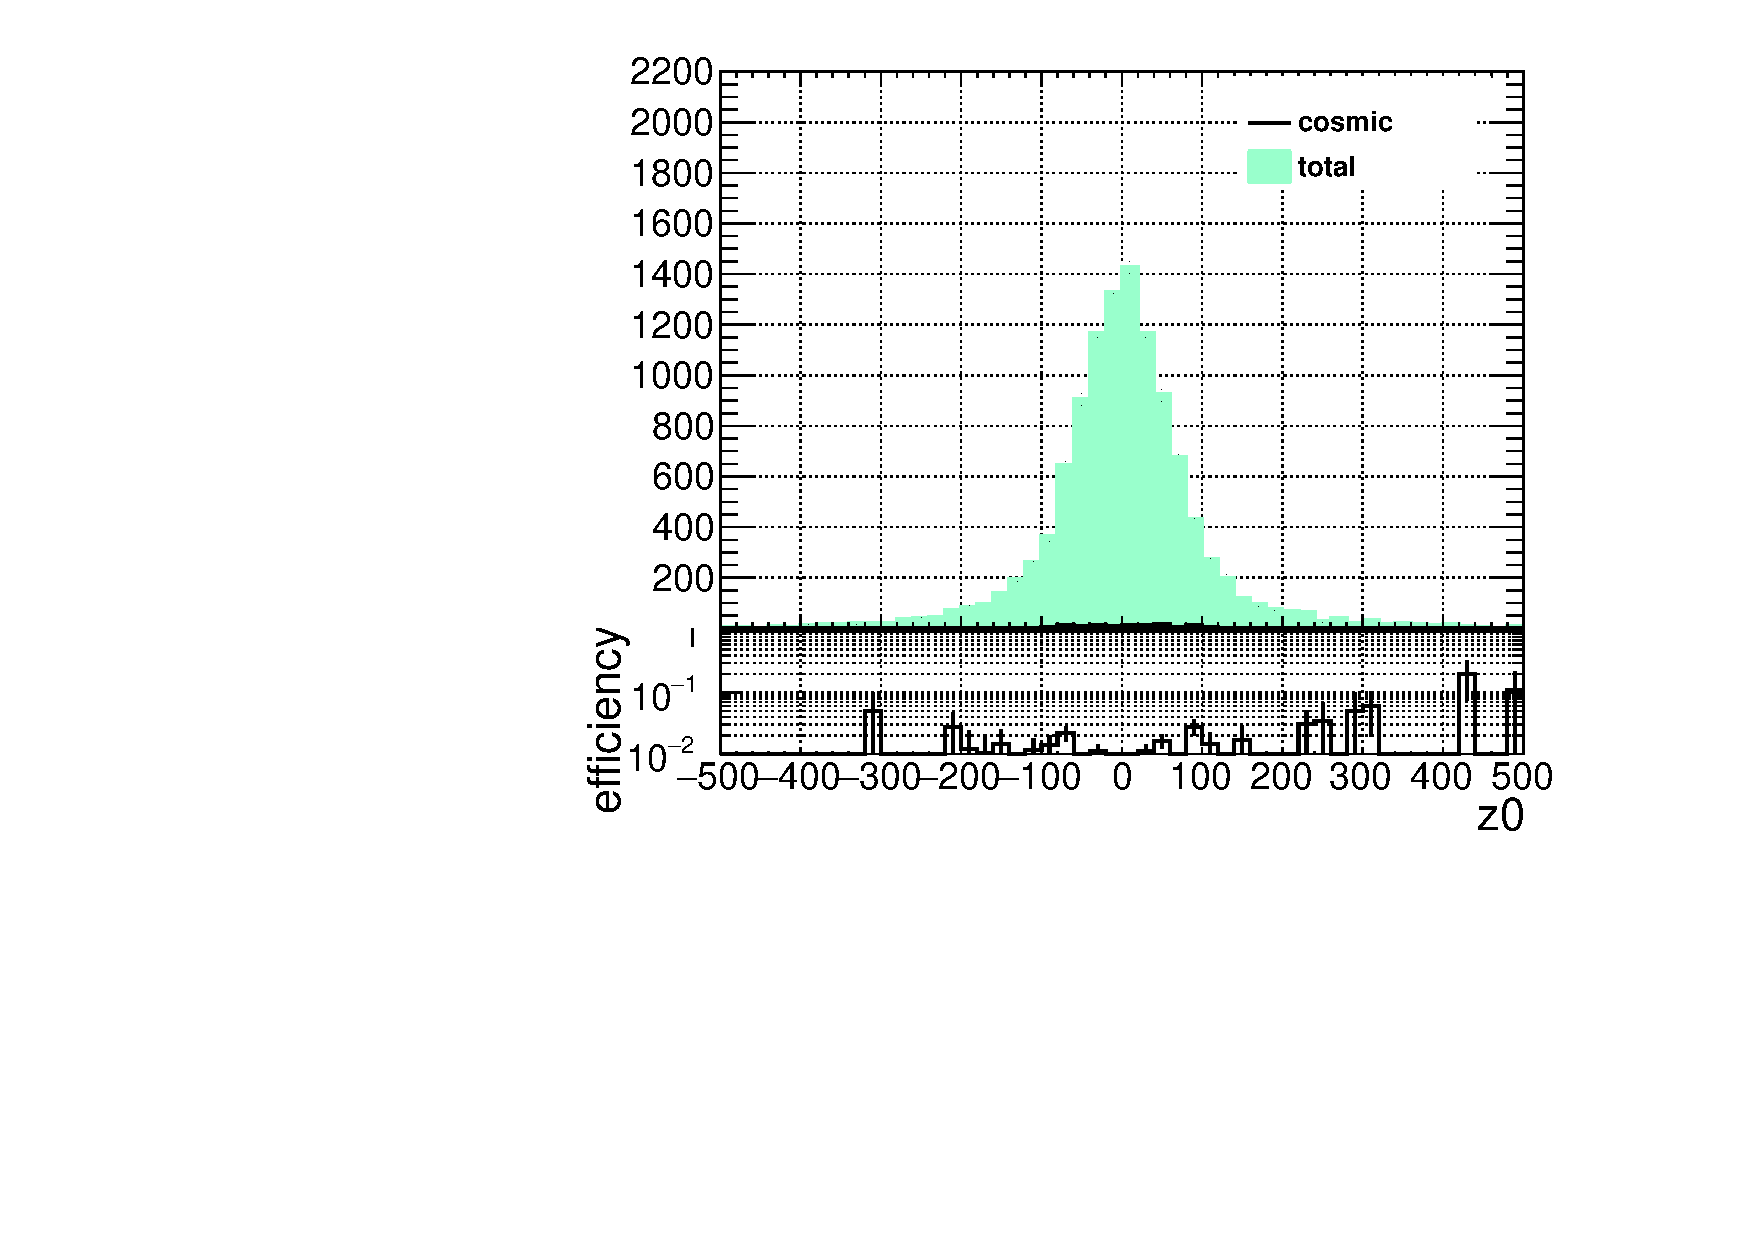
\includegraphics[width=.18\textwidth]{figures/cosmics/mc_300_ratio_z0.pdf}
%  	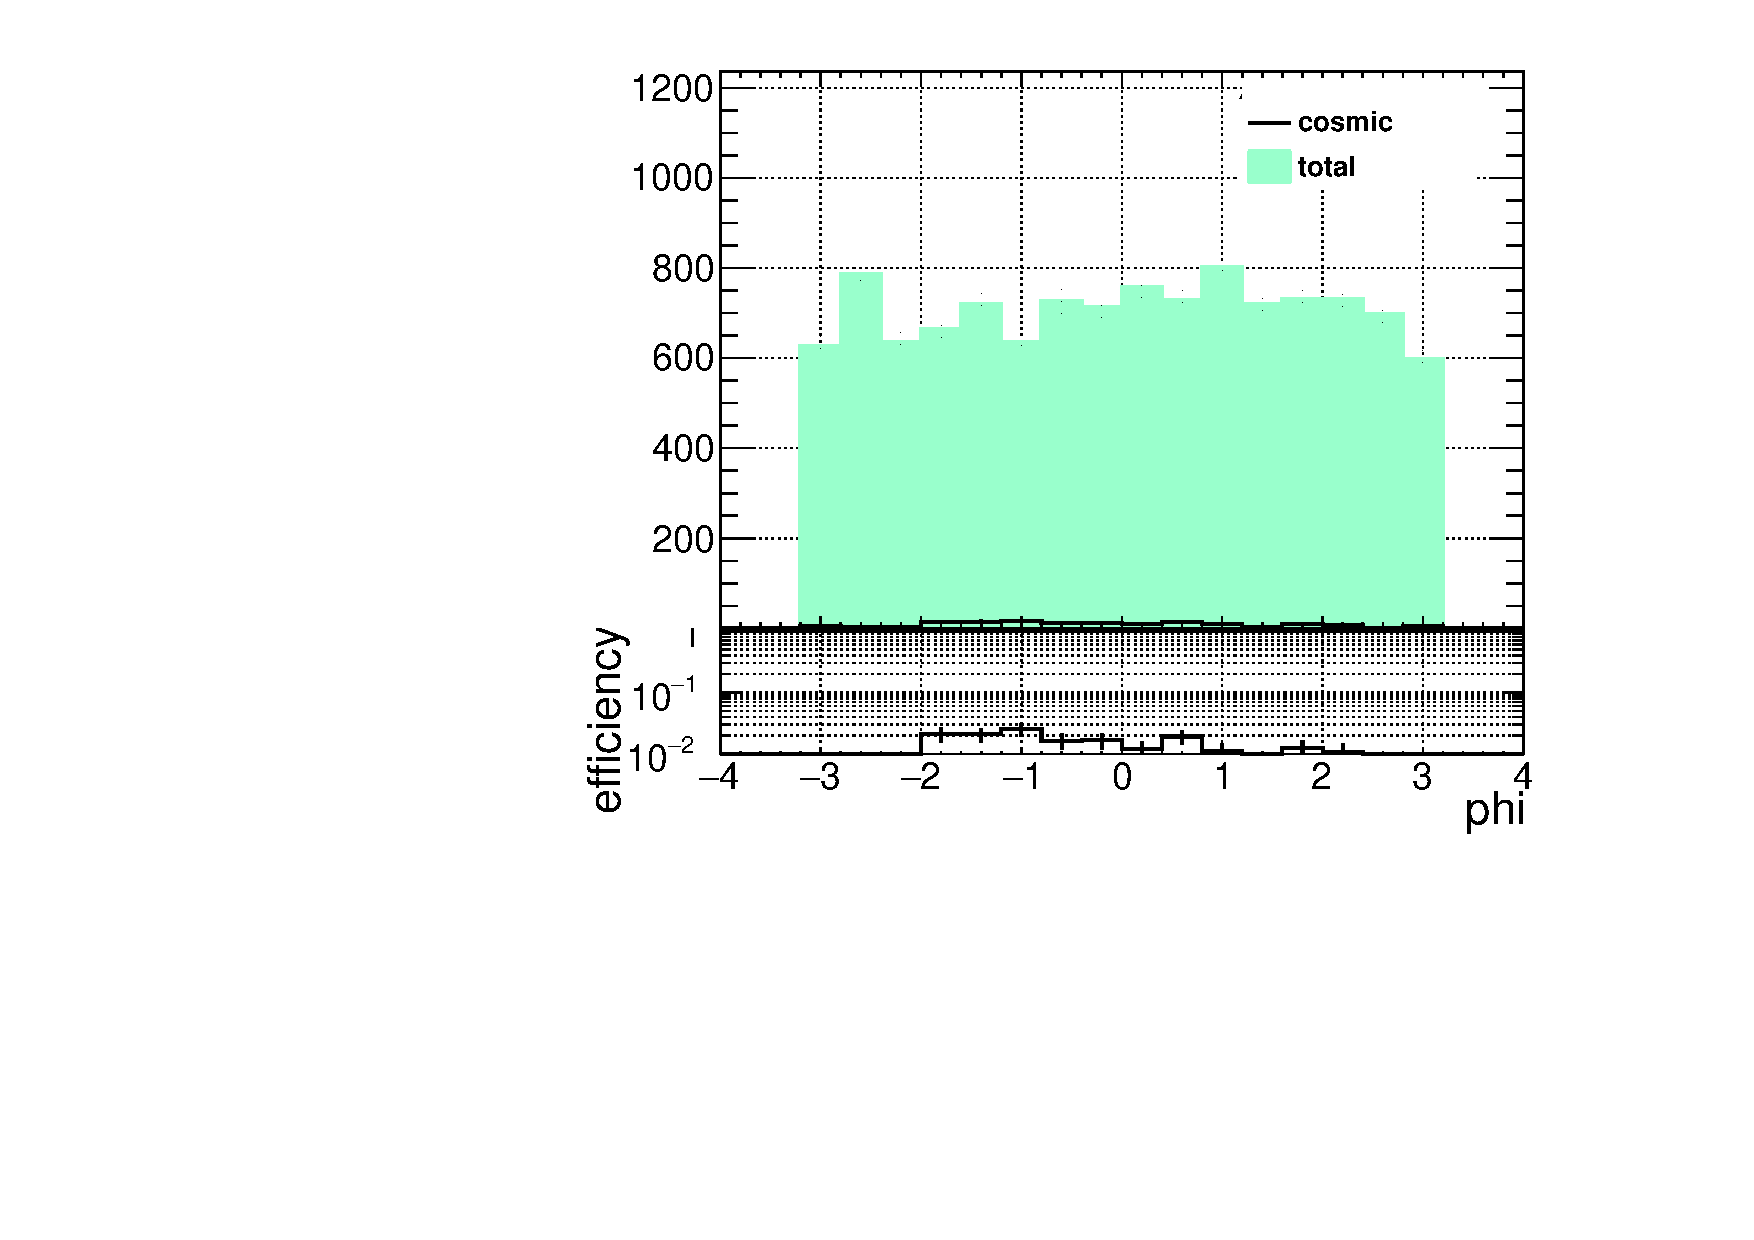
\includegraphics[width=.18\textwidth]{figures/cosmics/mc_300_ratio_phi.pdf}
%  	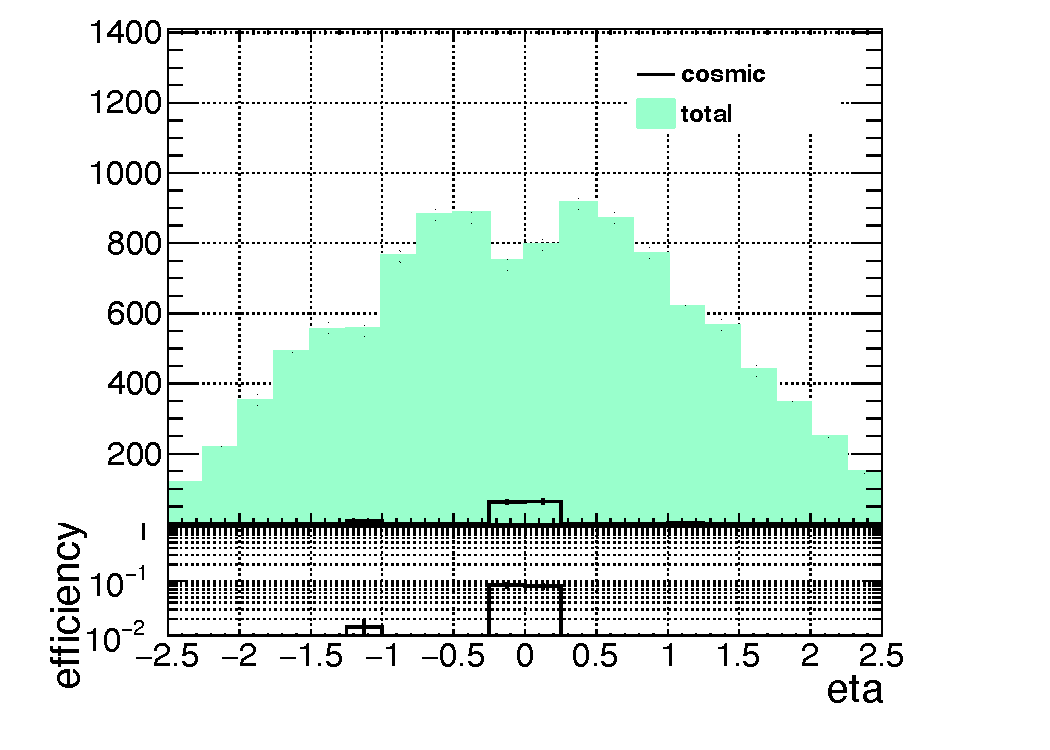
\includegraphics[width=.18\textwidth]{figures/cosmics/mc_300_ratio_eta.pdf}
%  	\caption{Cosmic tagging efficiency in signal \ac{MC}.}
%  \end{subfigure}
%    \caption{Cosmic tagging efficiency with respect to \pt, \dz, \z, $\phi$, $\eta$ in VR-$\mu$ data %(top) and signal \ac{MC}. The green shows the distribution of all muons, while the black line shows the subset of all muons that are cosmic tagged. A ratio of the two is shown below each plot.}
%  \label{fig:cos_eff}
%\end{sidewaysfigure}



\subsection{Properties of Events with Cosmic Tagged Muons}
Because all all events with a cosmic tagged muon are vetoed, a \ac{CR} with at least one cosmic tagged muon, CR-$M_{\textrm{full}}$, is defined to study cosmic events. There are about 224,000 events with at least one cosmic-tagged muon in the full dataset. 90\% of events in CR-$M_{\textrm{full}}$ have only one muon, and that muon is cosmic tagged. 90\% of those events find the cosmic muon on the bottom of the detector, \mb. The other 10\% of events have two reconstructed muons and they are both cosmic tagged. One event was seen that had four cosmic tagged muons, two on either side of the detector, indicating muons from a cosmic shower. In CR-$M_{\textrm{full}}$ events, some jets are seen from pileup collisions, but no additional leptons are observed in events with with cosmic muons. Interesting \ac{LHC} collisions are rare and so are cosmic muons, so the odds of having the two coincident in the same bunch crossing is minuscule. Generally, the cosmic muon is the most notable feature of the event and is the reason the event was triggered.

Events with two muons reconstructed from one cosmic muon have a very distinct signature. They have exactly correlated $z_{0}$, exactly anti-correlated $d_{0}$, equal and opposite $\phi$ measurement, and their $\eta$ measurements sum to 0. This can be seen in \autoref{fig:2cos}. No events were found with evidence of a cosmic muon's trajectory changing due to radiation in the detector, so this effect is assumed to be negligible within the detector resolution.


\begin{figure}[!ht]
\centering
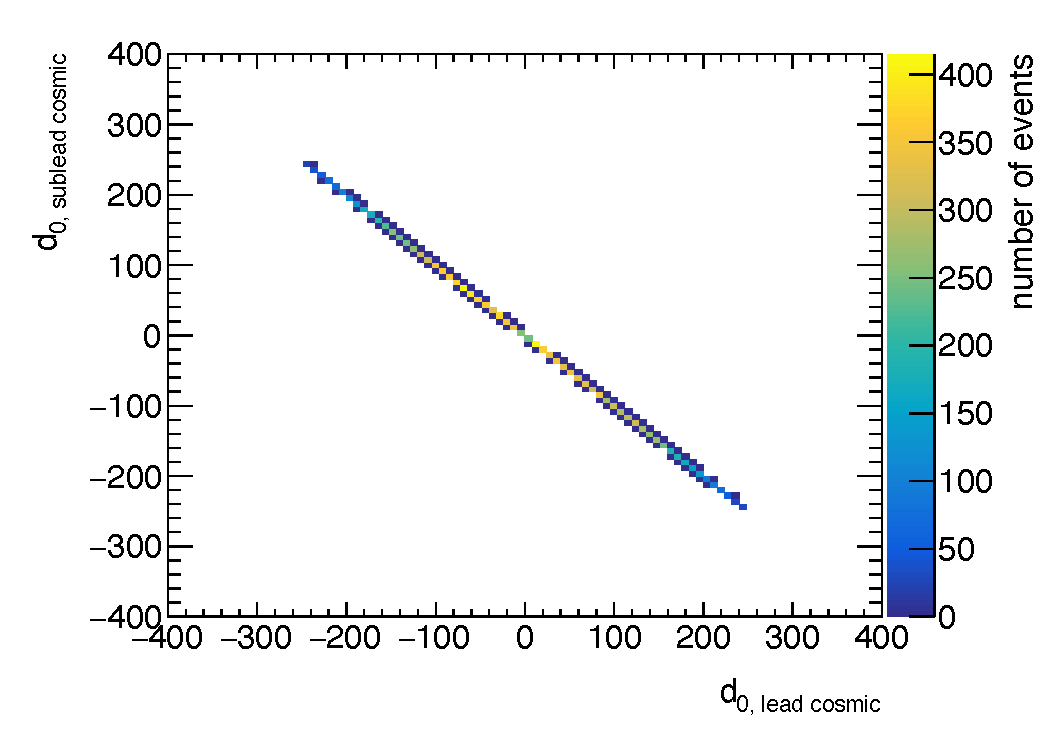
\includegraphics[width=.48\textwidth]{figures/cosmics/v4_widetag_2_2cos_d0_d0.pdf}
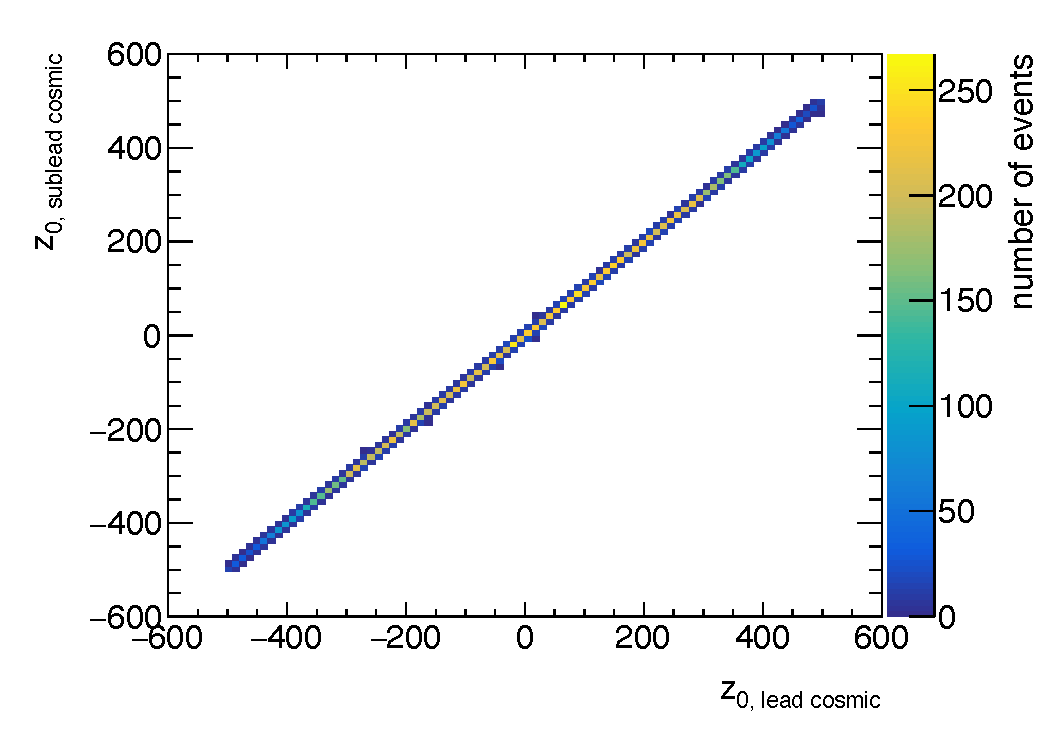
\includegraphics[width=.48\textwidth]{figures/cosmics/v4_widetag_2_2cos_z0_z0.pdf}
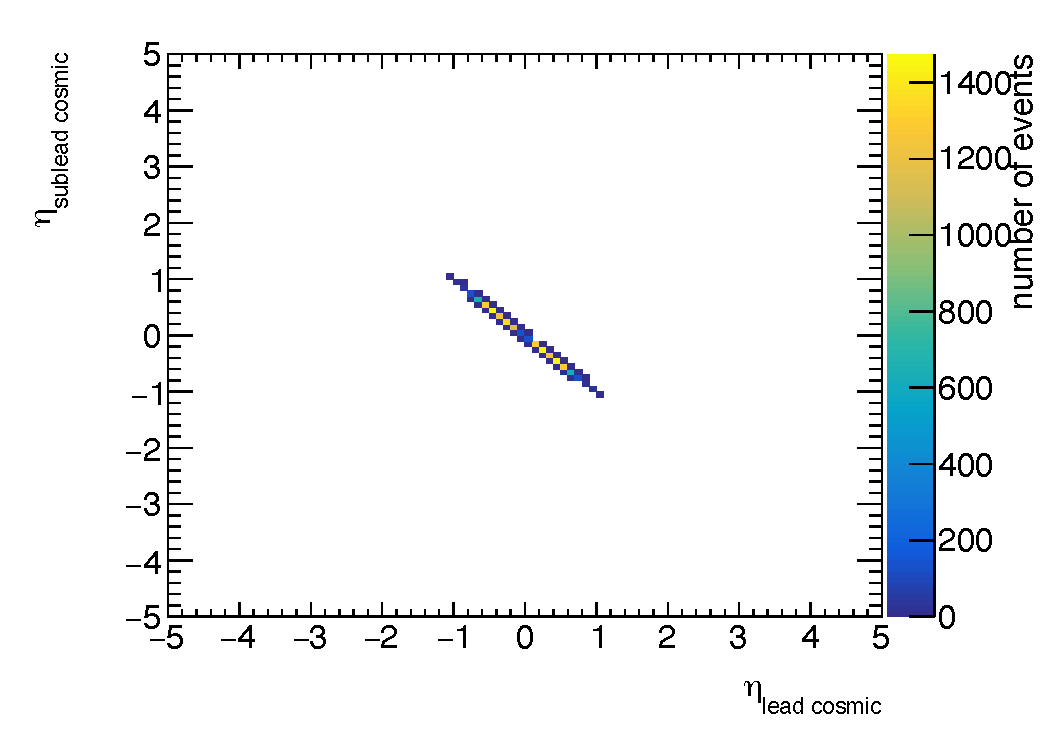
\includegraphics[width=.48\textwidth]{figures/cosmics/v4_widetag_2_2cos_eta_eta.pdf}
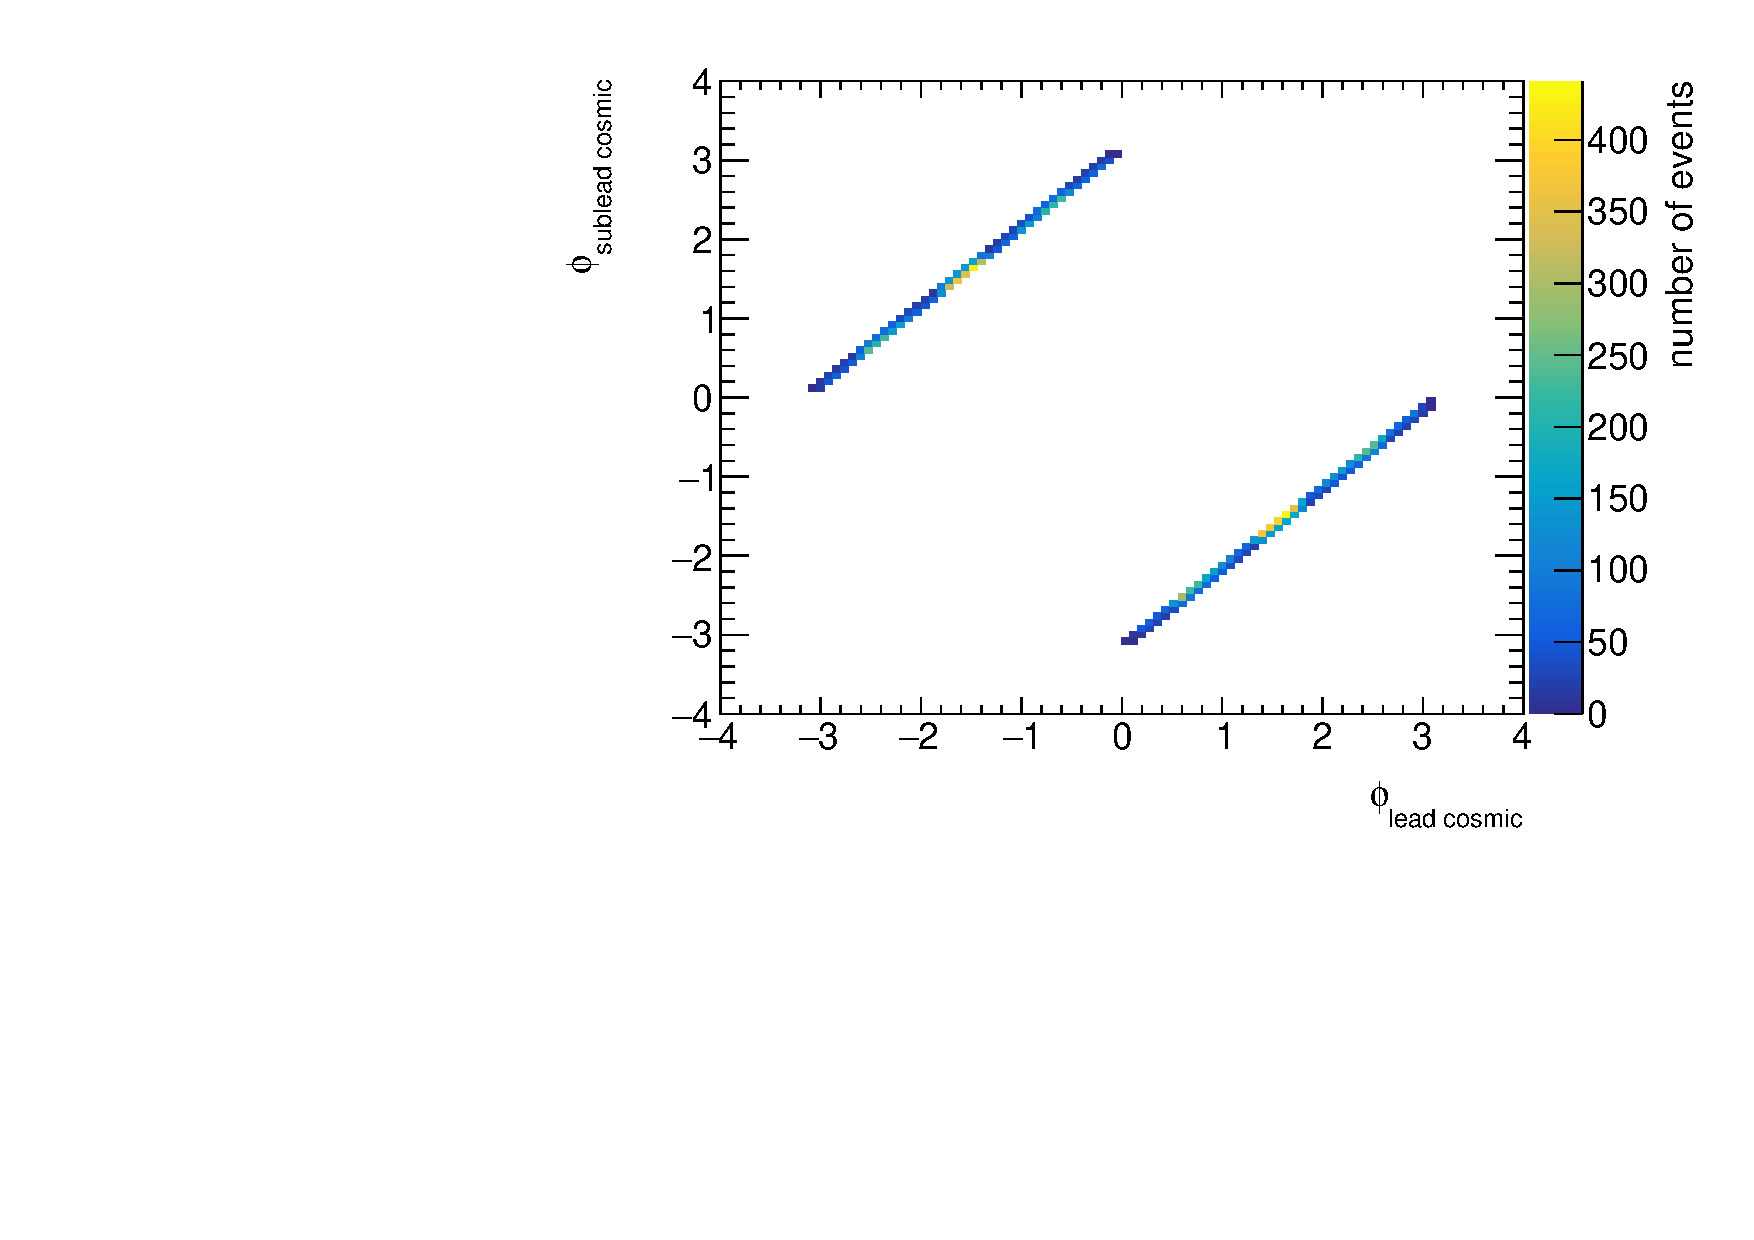
\includegraphics[width=.48\textwidth]{figures/cosmics/v4_widetag_2_2cos_phi_phi.pdf}
\caption{Relationship between two cosmic tagged muons in an event. Their \dz (top left), \z (top right), $\eta$ (bottom left), and $\phi$ (bottom right) values all indicate that the two muons originate from the same cosmic. }
\label{fig:2cos}
\end{figure}


The timing distributions as measured by the MDT segments of muons in 1 and 2 cosmic tagged events can be seen in \autoref{fig:cos_timing}. In the 1 $\mu$ case, \mb has a timing distribution centered around 0, indicating that \mb is responsible for the trigger decision in these events. However, in 1-$\mu$ events in which only \mt passes baseline selections, its timing distribution is shifted negative (early w.r.t the collision), mirroring the distribution for \mt in 2-$\mu$ events. This indicates that, even in cases in which only \mt is reconstructed, the trigger decision is made based on \mb. 

\begin{figure}[!ht]
\centering
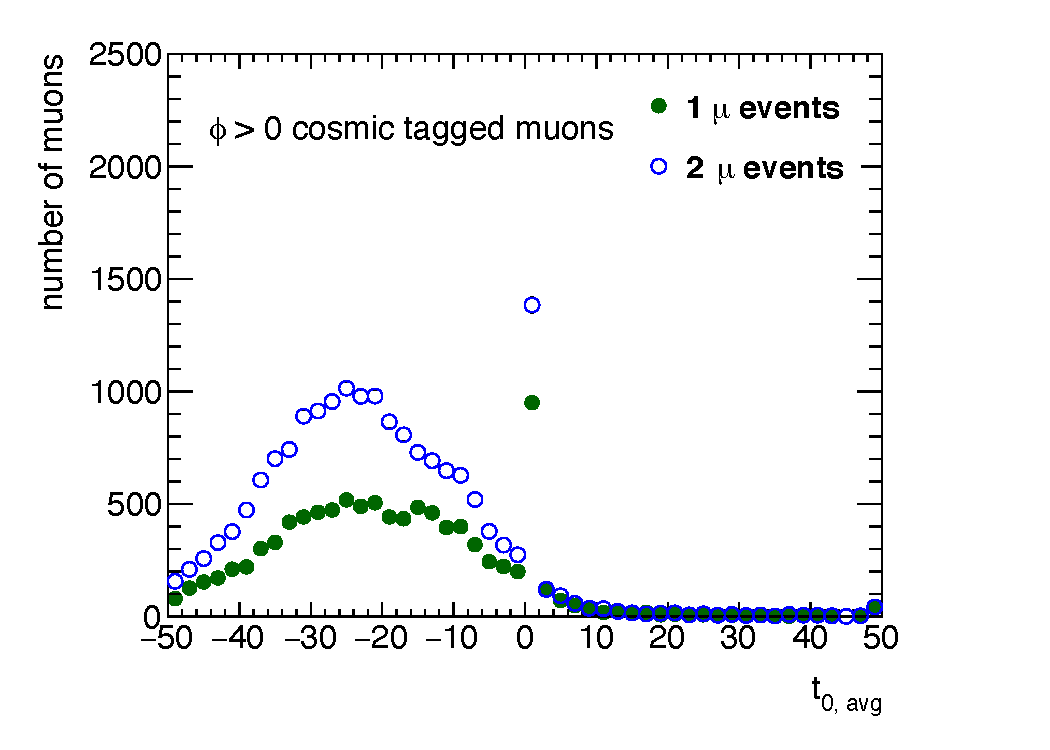
\includegraphics[width=.48\textwidth]{figures/cosmics/t0_plusphi.pdf}
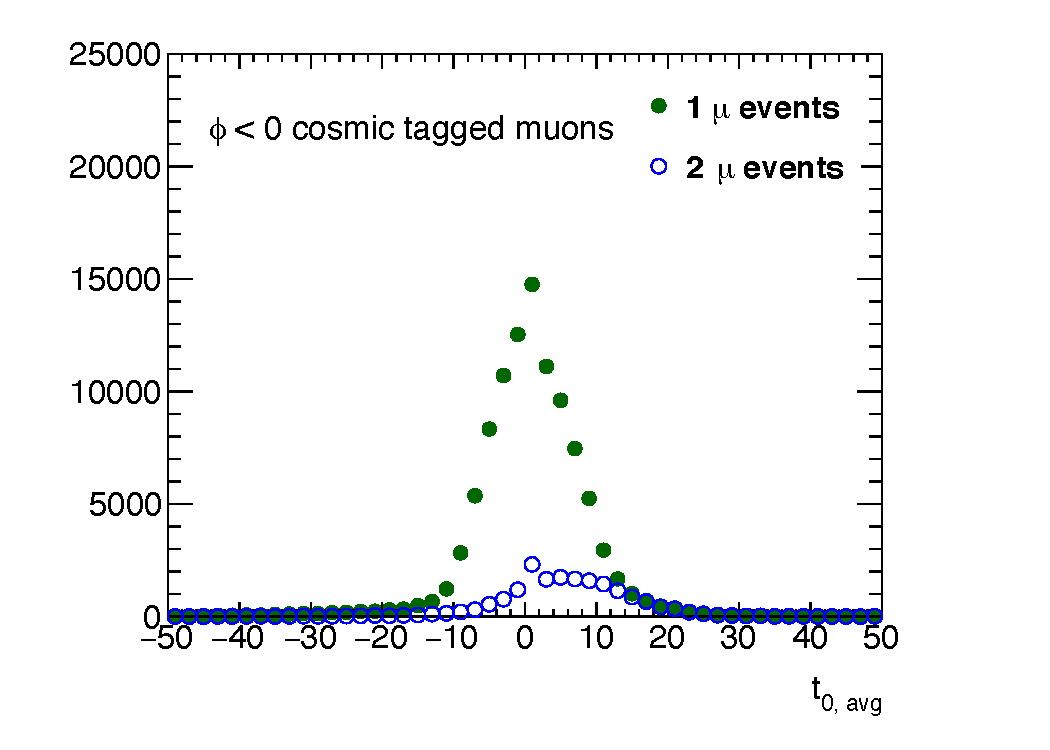
\includegraphics[width=.48\textwidth]{figures/cosmics/t0_negphi.pdf}
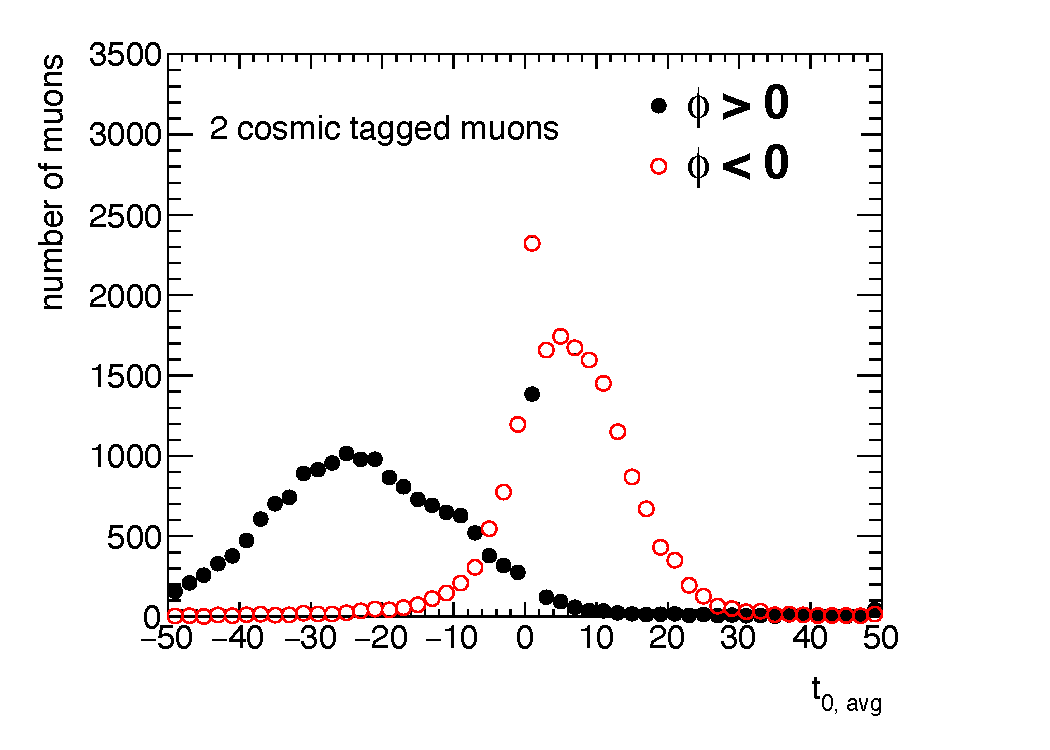
\includegraphics[width=.48\textwidth]{figures/cosmics/t0_2cos_plusminus.pdf}
\caption{Comparison of timing distributions of positive $\phi$ (top left) and negative $\phi$ (top right) muons in 1 and 2 cosmic events, as well as the timing distribution of top and bottom muons in 2 cosmic events (bottom). Here, ``2 cosmic tagged muons'' implies 2 muons reconstructed from 1 cosmic muon. \tavg is calculated by taking the average of the $t_{0}$ measured by all segments associated to the muon. Note that the peak at \tavg = 0 indicates a failure of the fit used to measure \tavg, these are handled separately and individual segments with \tavg = 0 do not enter the \tavg calculation.}
\label{fig:cos_timing}
\end{figure}

It takes roughly the same time for a cosmic muon to cross the width of the detector as is the bunch spacing (about 25 ns). This means that in order to have sufficient detector information to reconstruct two muons, the two \ac{MS} signatures must be at the edges of the detector readout window and near the bounds of the \tavg cut. This makes one or both muons likely to have detector information associated to the wrong event. Due to the early timing of \mt, this is more likely for \mt, but occurs for both \mt and \mb. 

Each of the combined muons will pass signal selections, because high quality information exists from the \ac{ID}, but if enough \ac{MS} information is missing, the \ac{MS} segments will not be found back to back with the opposite combined muon, causing one or both of the muons to evade the cosmic tag. Ultimately, it is this mismeasurement that leads to the background in SR-$\mu\mu$. 


\subsection{Background Estimate}

If a \ac{MS} segment is reconstructed without direct $\phi$ measurements from \ac{RPC} or \ac{TGC} hits, its $\phi$ measurement is taken as the center of the \ac{MDT}, which has resolution of $\Delta \phi = 0.2$ (the final nominal tag value of $\dphicos = 0.25$ was expanded to include these cases). Events with this measurement scheme were seen in a preliminary definition of the cosmic tag, which used the same \sigeta cut, but the \dphicos cut was reduced to $\dphicos = 0.18$. With this preliminary version of the cosmic tag, about 40 events were observed with one cosmic tagged muon, and another untagged muon. In these events, \mt was missing direct \ac{MS} $\phi$ measurements, so its segments were not back-to-back with \mb and \mb was not tagged as a cosmic. \mb however, was well measured, so \mt was cosmic tagged. An event can enter the signal region if both \mb and \mt are sufficiently mis-measured that neither can be tagged. This is sketched in \autoref{fig:cosmic_mismeasure}. A muon's cosmic tag is dependent on the opposite muon's quality, so the muon's cosmic tag status and its quality are assumed to be uncorrelated in order to make an estimate of the background.

This estimate and validation makes use of the two cosmic tags described in \autoref{tab:costag_values}, as well as an \emph{intermediate tag} which defines a muon that is not tagged by the narrow tag but is tagged by the nominal tag. Because a cosmic muon is defined using detector information on the opposite side of the detector, muons tagged using the narrow tag must have a higher quality measurement on the opposite side of the detector in order to pass the tighter cuts than those tagged with only the nominal tag. Cosmic tagged muons with $\dphicos-\sigeta$ values closer to the edge of the nominal cosmic tag window are more similar to those that would enter SR-$\mu\mu$ as background (which are outside of the cosmic tag window). 



\begin{figure}[!ht]
\centering
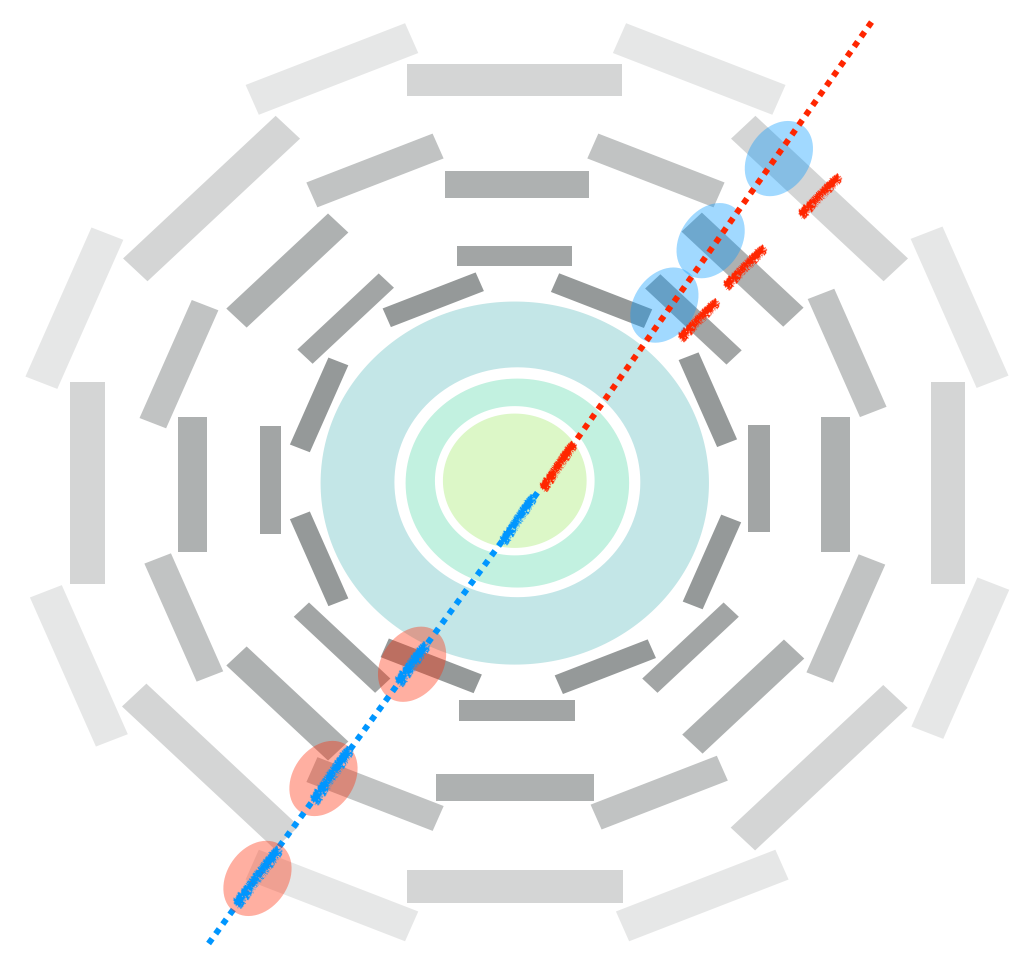
\includegraphics[width=.4\textwidth]{figures/cosmics/1badcos.png}
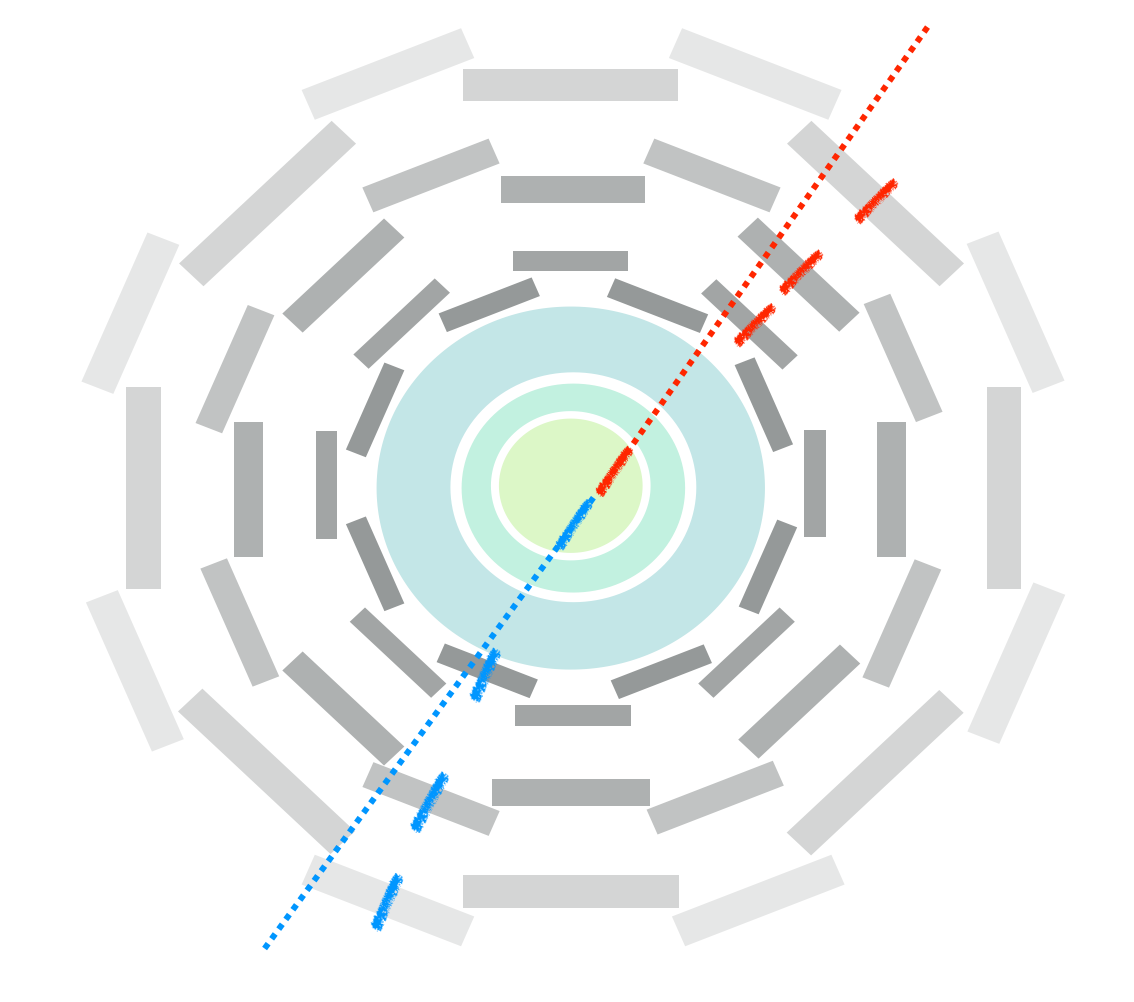
\includegraphics[width=.45\textwidth]{figures/cosmics/2badcos.png}
\caption{Sketches illustrating how a a 2 $\mu$ cosmic event could evade a cosmic tag. In this diagram, the thick lines represent ID tracks and MS segments, and the dashed line the CB muon measurement. A muon is tagged as cosmic if it is back to back with an MS segment. If an MS segment does not have a direct $\phi$ measurement from an RPC hit, its $\phi$ measurement is taken as the center of the MDT, which has an uncertainty of 0.2 (though the muon can be mismeasured in other ways as well, for example lacking MDT hits or resulting from a bad combination of ID track and MS track). The sketch on the left shows a 2 $\mu$ event where the red muon is cosmic tagged but the blue is not. The segments attached to the red muon are not measured well, so when we look for the red segments back to back with the blue muon (the blue circles), the segments are not in the right place and the blue muon is not cosmic tagged. However, the blue muon is well measured, so when we look back to back with the red  muon, we find the segments of the blue muon. Thus, the better quality muon is not tagged, while the poorer quality muon is. The right shows a scenario where both muons have this mismeasurement, and so neither is cosmic tagged. This is what contributes to the background in SR-$\mu\mu$.}
\label{fig:cosmic_mismeasure}
\end{figure}


To estimate the number of events entering SR-$\mu\mu$ from poorly measured cosmic muon events, a scaling factor from good quality to bad quality muons, \rgood, is defined. Then, it is used to scale events which have one good quality and one bad quality muon, CR-$\mu\mu$-topbad, into SR-$\mu\mu$ to esimate the background contribution. This is  in \autoref{fig:cosmic_est}. ``Good'' quality defines a muon that passes signal cuts on \nprecision, \nphi, and \chiCB, while a ``bad'' quality muon fails at least one of these cuts. For the nominal version of the estimate, it is assumed that there is one $\phi > 0$ muon (\mt) and one $\phi < 0$ muon (\mb), and \mt is the muon is scaled from ``bad'' to ``good'' quality. All regions have 2 reconstructed muons, and the cosmic tag and quality are varied to define the various regions used to make the estimate.

\begin{figure}[!ht]
\centering
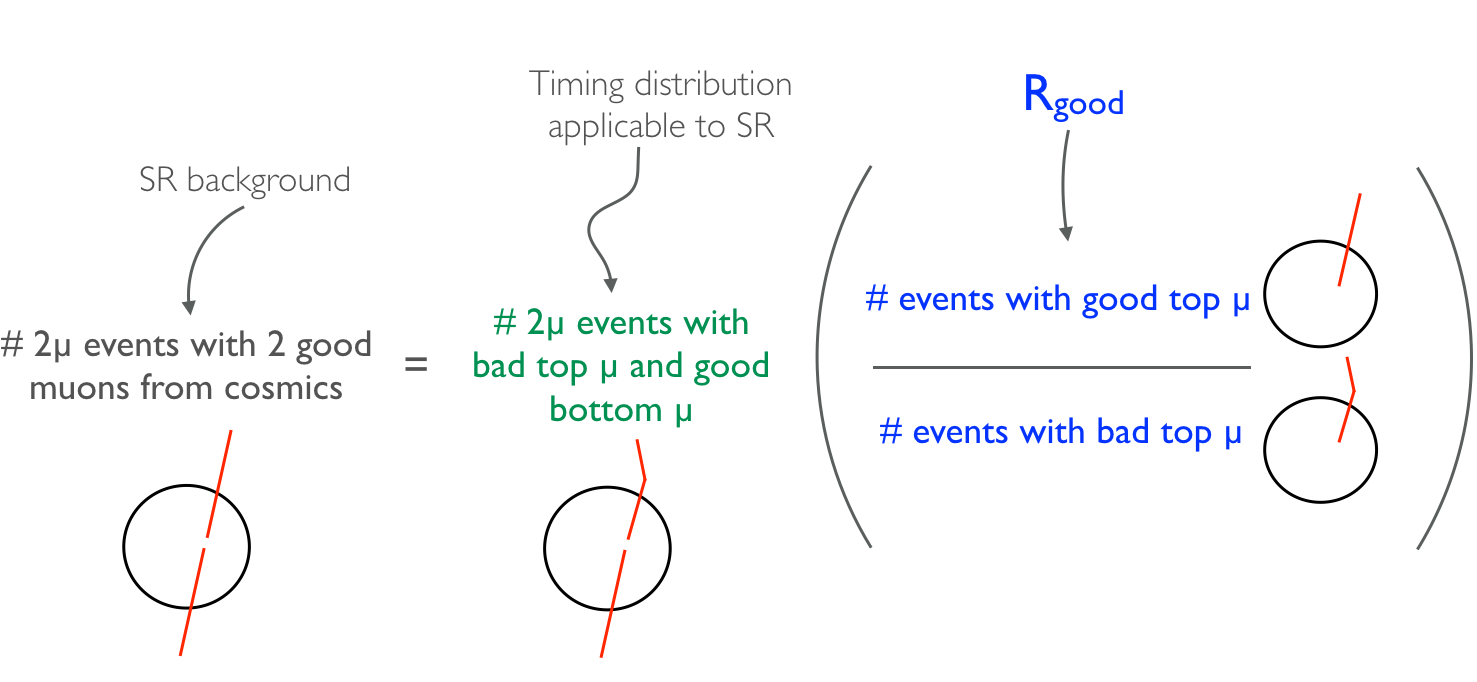
\includegraphics[width=.8\textwidth]{figures/cosmics/background_sketch.png}
\caption{A visual representation of the background estimation strategy}
\label{fig:cosmic_est}
\end{figure}

\rgood for the SR-$\mu\mu$ estimate is defined using muons tagged with the full cosmic tag. A validation estimate is also defined, using the narrow and intermediate cosmic tags. The signal and validation regions used in this estimate are sketched in \autoref{fig:cosmic_SRVR} and the numbers of events in each region listed in \autoref{tab:estimate_counts}. Aside from Region 2 (CR-$\mu\mu$-topbad), all other regions in the SR and VR estimates are subsets of CR-$M_{\textrm{full}}$. These regions were chosen to maintain orthogonality, while minimizing signal contamination and maximizing statistical power. In all cases, statistical errors on \rgood are computed using the Wilson interval which is recommended for values close to zero with small statistics \cite{ROOTAsymmErrors}. 

\begin{figure}[!ht]
\centering
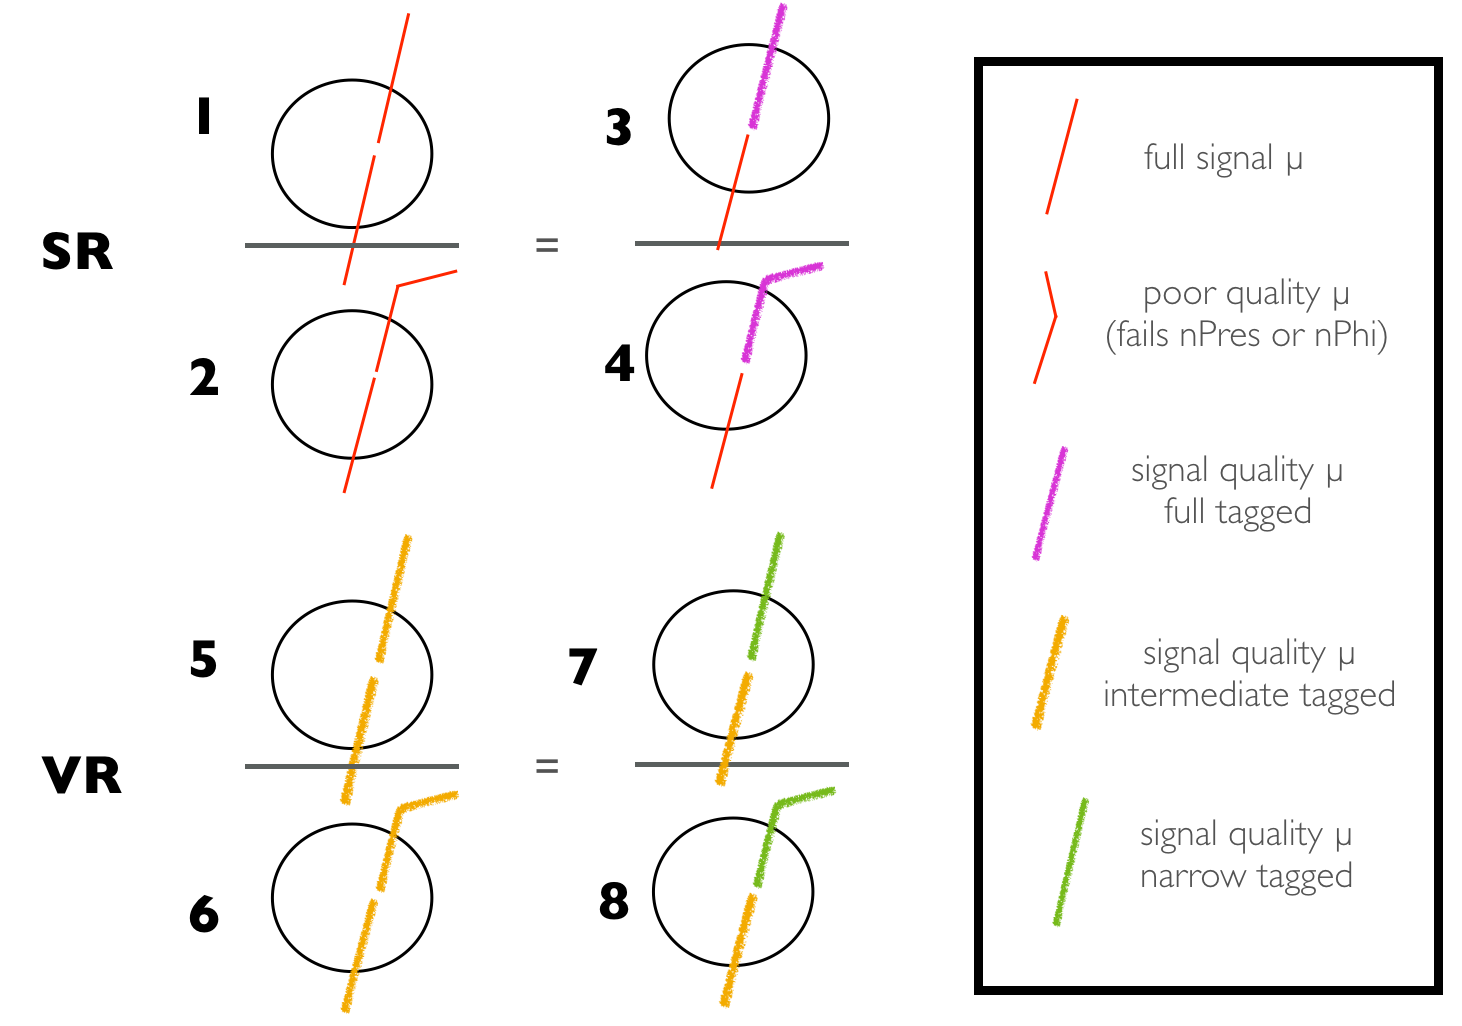
\includegraphics[width=.8\textwidth]{figures/cosmics/SR-VR-sketch.png}
\caption{A visual representation of the CRs and VRs used to estimate and validate the background contribution to SR-$\mu\mu$ due to cosmic muons. Regions 3 and 4 are used to define \rgood. These regions were chosen to maintain orthogonality, while minimizing signal contamination and maximizing statistical power.}
\label{fig:cosmic_SRVR}
\end{figure}

\begin{table}
\centering
\begin{tabular}{ccc}
Region & $\phi < 0$ muon & $\phi > 0$ muon \\
\hline
1 & signal & signal\\ 
2 & signal & fails at least one MS quality cut\\ 
3 & signal & cosmic tagged \\ 
4 & signal & cosmic tagged and fails at least one quality cut\\ 
5 & narrow tagged & narrow cosmic tagged\\ 
6 & narrow tagged & narrow cosmic tagged and fails at least one quality cut\\ 
7 & narrow tagged & full, but not narrow, tagged \\ 
8 & narrow tagged & full, but not narrow, tagged and fails at least one quality cut\\  
\hline
\end{tabular}
\caption{A description of the regions used for the cosmic estimate and validation. Each column describes the way in which the muon deviates from a signal muon, meaning a muon is signal in all respects except for the parameter(s) listed in the table.}
\label{tab:cosmic_SRVR}
\end{table}


\begin{table}
\centering
\begin{tabular}{cccccccccc}
Region & 1    & 2 & 3 & 4 & 5 & 6 & 7 & 8\\
\hline
Event Yield & --  & 2 & 1 & 18 & 1088 & 1000 & 1947 & 2465 \\
\hline
\end{tabular}
\caption{Numbers of events in each region used for the cosmic estimate. Regions 2-4 are used to estimate SR-$\mu\mu$ (Region 1) and Region 6-8 estimate the number of events in Region 5, show in \autoref{fig:cosmic_SRVR}.}
\label{tab:estimate_counts}
\end{table}

Results of the estimate and validation are shown in \autoref{tab:estimate_results}. There is a statistically significant discrepancy between the estimated and actual number of events in the VR. This nonclosure can be explained by the difference in \absdz distributions in Region 5 and Region 6, shown in \autoref{fig:cos-nonclosure-plots}. The excess of low \absdz, high \chiCB muons in the weighted Region 6 compared to Region 5 implies that more muons have been created due to a poor combination of prompt track with MS track. The estimate was performed in the VR with \rgood  defined as a function of \absdz and the nonclosure was reduced from 37.7\% to 11.7\%. It is not possible to perform this estimate as a function of \absdz in the SR due to low statistics in Region 2 and Region 3. The estimate is performed without the \absdz binning and the nonclosure from the unbinned estimate in the VR is taken as an uncertainty (37\%). In the SR, seen in \autoref{fig:SR-rgood}, there are no overlapping \absdz bins in CR-$\mu\mu$-topbad and \rgood, however, adjacent bins are filled, so the extrapolation over \absdz is not large and uncertainity from this extrapolation is contained in the nonclosure systematic. \rgood and \absdz distributions for each estimate is shown in \autoref{fig:SR-rgood} and \autoref{fig:VR-rgood} for the SR and VR, respectively.

\begin{table}
\centering{}
\begin{tabular}{ccccccc}
Region & central value & up error & down error & actual value & \% diff from actual \\
\hline
VR        & 789.9  & 34.85 & 34.4 & 1088 & 37.7\%  \\
SR        & 0.11 & 0.20  & 0.10  & --   & --   \\
\hline
\end{tabular}
\caption{Results of the background estimation strategy in the two validation regions and the signal region}
\label{tab:estimate_results}
\end{table}

\begin{figure}[!ht]
\centering
\includegraphics[width=.48\textwidth]{figures/cosmics/ratio_d0.pdf}
\includegraphics[width=.48\textwidth]{figures/cosmics/d0_ratio_binned.pdf}
\caption{Comparison of \absdz in Region 5 (orange) compared with Region 6 weighted by unbinned \rgood = 0.78 (left) and by \rgood defined as a function of \absdz (right). The nonclosure improves from 37.7\% to 11.7\% by binning \rgood in \absdz. The error shown is statistical only. There is no trend in other variables (\pt, $\eta, \phi$, \z, \tavg).}
\label{fig:cos-nonclosure-plots}
\end{figure}

\begin{figure}[!ht]
\centering
\includegraphics[width=.48\textwidth]{figures/cosmics/d0_VR_v4_rgood.pdf}
\includegraphics[width=.48\textwidth]{figures/cosmics/d0_VR_v4_2mu.pdf}
\caption{\absdz distribution of \rgood (left) and \mt in Region 6 to perform the VR estimate. To calculate the background estimate, the distributions are multiplied bin by bin and summed. The error shown is statistical only. This method is ultimately not used, in favor of an unbinned version, due to statistical limitations in the regions used for the SR estimate}
\label{fig:VR-rgood}
\end{figure}

\begin{figure}[!ht]
\centering
\includegraphics[width=.48\textwidth]{figures/cosmics/d0_SR_v4_rgood.pdf}
\includegraphics[width=.48\textwidth]{figures/cosmics/d0_SR_v4_2mu.pdf}
\caption{\absdz distribution of \rgood (left) and \mt in Region 2 to perform the SR estimate. To calculate the background estimate, the distributions are multiplied bin by bin and summed. The error shown is statistical only. It can be seen here that there are no overlapping bins between the two plots, and so this method is ultimately not used, in favor of an unbinned version.}
\label{fig:SR-rgood}
\end{figure}

\subsection{\label{sec:cos_syst}Systematic Uncertainties}

\paragraph{Muon Orientation}

The estimate is performed using the quality of \mt since muons in the upper hemisphere are expected to be more temporally marginal and mismeasured. However, the strategy can be performed with the quality of \mb. Because bad quality \mb are more rare bad poor quality \mt, it is not possible to compare this strategy in the SR estimate, which is already statistically limited. However, the comparison can be made in the VR. As shown in \autoref{tab:syst-orientation}, this change produces an estimate that is consistent with the nominal estimate within statistical uncertainties. Nonetheless, a 13\% systematic uncertainty is applied from the difference between the two predictions.

The estimate relies on the assumption that if two muons are reconstructed from a cosmic muon, one will be on the top of the detector and the other on the bottom. 0 events were observed with one good muon and one bad muon on the same side of the detector (sign$(\phi_{0}$) = sign$(\phi_{1}$)) in both the 1 cosmic-tag regions and 0 cosmic-tag regions, so contributions from same-side muons are considered negligible.

\begin{table}
\centering
\small
\begin{tabular}{ccccccc}
central value  & up error & down error & actual value & \% diff from actual & \% diff from nominal\\
\hline
689.0  & 115.1 & 108.8 & 1088 & 62.3 \% & 13\% \\
\hline
\end{tabular}
\caption{Estimate in VR with bottom muon as test muon instead of top muon. CR-$\mu\mu$-topbad becomes VR-$\mu\mu$-bottombad and \rgood is defined using the quality of \mb instead of \mt.}
\label{tab:syst-orientation}
\end{table}


\paragraph{Quality parameter dependence}

In the nominal estimate, a ``bad'' quality muon means one that fails any one of the \nprecision or \nphi or \chiCB cuts. To evaluate the dependence one each variable, the estimate can be performed using only one of these to define a ``bad'' quality muon, requiring the others to pass the signal requirements. However, \chiCB is dependent on the MS track hit requirements and has a small contribution to the estimate regions on its own. Only inverting only \chiCB leaves 11 events in each Region 6 and Region 8 and 0 in Region 2 and Region 4. Thus, we account for the \chiCB contribution by remaining agnostic to it in performing the estimate with the other two quality variables.  Allowing for the failure of the \chiCB cut increases the \nprecision-only and \nphi-only estimates by 2\% and 1\%, respectively. \autoref{tab:estimate_variables_VR} and \autoref{tab:estimate_variables_SR} show the results of this procedure in the VR and SR, respectively. We take the largest difference from the nominal estimate in the VR (16.5\%) to account for the quality variable dependence. 

\begin{table}
\centering
\small
\begin{tabular}{cccccccc}
Variable & central value  & up error & down error &  actual value & \% diff  & \% diff \\
  &    &   &   &   & from actual & nominal\\

\hline
\nphi          & 783.6 & 69.2 & 68.1 & 1088 & 38.8\% & 0.9\% \\
\nprecision    & 920.6 & 51.8 & 50.9 & 1088 & 18.2\% & 16.5\% \\

\hline
\end{tabular}
\caption{Dependence of the background estimate in the VR on each of the variables used. In each estimate, only the given quality variable is used to define a ``bad'' muon and the other must always pass. In both cases, the \chiCB is allowed to pass or fail the signal cut.}
\label{tab:estimate_variables_VR}
\end{table}

\begin{table}
\centering
\begin{tabular}{cccccc}
Variable & central value  & up error & down error & \% diff from nominal\\
\hline
\nphi          & 0 & -- & -- & 100\% \\
\nprecision    & .33  & 0.75 & 0.40 & 200\% \\
\hline
\end{tabular}
\caption{Dependence of the background estimate in the SR on each of the variables used. In each estimate, only the given quality variable is used to define a ``bad'' muon and the other must always pass. In both cases, the \chiCB is allowed to pass or fail the signal cut.}
\label{tab:estimate_variables_SR}
\end{table}


\subsection{Summary}

This estimate is dominated by statistical uncertainties in the SR estimation regions. Ultimately, $0.11^{+0.20}_{- 0.11}$ ($^{+0.198}_{-0.104}$ stat. and 0.047 syst) events are expected in SR-$\mu\mu$ due to cosmic muons.


\FloatBarrier 
\section{Negligible Backgrounds}
Since this analysis is built on the assumption that there should be 0 background events in all signal regions, it is extremely important to ensure that all possible backgrounds are accounted for. Three different backgrounds were studied and determined to be negligible, meaning that they contribute $\mathcal{O}(10^{-4})$ or less events to the relevant \acp{SR}. 

\subsection{Material Interactions}

Material interactions define events with dilepton pairs that come from interaction with the material of the \ac{ATLAS} detector. In other searches for long lived particles in \ac{ATLAS} where displaced vertices (\acp{DV}) are required, \ac{DV}s are reconstructed by extrapolating their tracks to their intersection, and it can be determined if verticies originate from material. In this analysis, there is no vertex so such a veto cannot be used. In order to study material interactions, events with leptons associated to displaced vertices from material were studied. It was found that in the cases of both electrons and muons, events with an \ac{DV}, where one track is associated to a lepton, the \dR between the lepton and the other track in the \ac{DV} was less than 0.2. After making the requirement that $\dR_{\ell, \text{track}} < 0.2$, no \acp{DV} with signal leptons were found. In the case of the background to one of the \acp{SR}, the second track in the \ac{DV} would be associated to a lepton. After this cut is made, this background is negligible to all 3 \ac{SR}.

\subsection{Fake Muons}
Fake muons were estimated using an ABCD method similar to SR-$ee$ and SR-$e\mu$. Muons were selected using the baseline requirements, plus asking that be isolated, and not cosmic tagged. All remaining cuts used for defining signal muons were used to define ``passing'' muons. Using this strategy, only 6 events were seen in the D region, and 0 in either B or C. In the SR-$e\mu$ fake estimate, the ratio of passing to failing muons is less than 1\%. Given this, the probability for two fake muons to pass our selections should be less than 0.01\%, making this background negligible ($<0.0006$ events) and we consider it to be negligible relative to cosmic muons.

\subsection{Heavy Flavor Muons}

Heavy flavor electrons and muons cannot be disentangled from algorithmic fakes in SR-$ee$ and SR-$e\mu$ and are estimated in conjunction with fakes. Fakes are negligible in SR-$\mu\mu$, so a \ac{HF} estimate must be performed separately. Very few events in \ttbar \ac{MC} have single muons from decays of b-hadrons pass the signal \pt and \absdz cuts, so this background is expected to be small when two muons are required. An ABCD method cannot be used for this estimate because it cannot be assumed that the probability to find an isolated muon is uncorrelated between 2 muons from two \ac{HF} decays.

First, data was checked for anti-isolated muon events in CR-$\mu\mu$-hf, a region with two signal muons and at least one of the muons must be anti-isolated. No events were observed. Loosening the kinematic cuts to $\pt > 50 \GeV$ and $\absdz > 2$ mm also found zero events. Finally, since the muon trigger and thus muon \texttt{DRAW\_RPVLL} filter only requires one muon, it was possible to study events with one baseline muon and one muon with $\absdz > 0.5$ mm. One event was observed in this region. Then, extrapolation factors to the \ac{SR} kinematic cuts were defined from the same dataset. The extrapolation factor  from the extremely loosened region into SR-$\mu\mu$ for both the \absdz and \pt of both muons was calculated to be $0.00013 \pm 0.00013$. This means that $1.3 \times 10^{-4}$ are expected in SR-$\mu\mu$ from muons from \ac{HF}, a negligible contribution.


\section{Summary}

In all, $<1$ events are expected in each \ac{SR}. \autoref{tab:bkg-summary} summarizes the background estimates and \autoref{tab:uncertainties} summarizes the systematic uncertainties.

\begin{table}
\centering
\begin{tabular}{lccc}
Region 			 & SR-$ee$ 			& SR-$\mu\mu$ 				& SR-$e\mu$ \\
\hline
Total background & $0.46 \pm 0.10$ 	& $0.11 ^{+0.20}_{-0.11}$	& $0.007^{+0.019}_{-0.011}$\\
\hline
Fakes + Heavy Flavor 			 & $0.46 \pm 0.10$ 	& $< 10^{-4}$ 						& $0.007^{+0.019}_{-0.011}$\\
Cosmics 		 & - 				& $0.11 ^{+0.20}_{-0.11}$ 	& - \\
\hline
\end{tabular}
%%%%
\caption{Summary table of the background estimate and uncertainty in each \ac{SR}.}
\label{tab:bkg-summary}
\end{table}

\begin{table}[htb]
\small
\begin{center}
\begin{tabular}{lcc}
Background & Uncertainty & Value [\%] \\
\hline
\multicolumn{3}{c}{SR-$ee$} \\
\hline
\multirow{3}{*}{Fake and Heavy Flavor} 	& Statistical 	& 18 \\
 						& HF Nonclosure & 11 \\
 						& Fake Nonclosure& 6 \\
 						& Total 		& 22 \\
\hline
\multicolumn{3}{c}{SR-$e\mu$} \\
\hline
\multirow{3}{*}{Fake and Heavy Flavor} 	& Statistical 	& +260 / -130 \\
 						& HF Nonclosure & 92 \\ 
 						& Fake Nonclosure & 8 \\
 						& Total 		& +270 / -160 \\
\hline
\multicolumn{3}{c}{SR-$\mu\mu$} \\
\hline
\multirow{4}{*}{Cosmic Muons} 	& Statistical 			& +180 / -95 \\
 								& VR Nonclosure		& 38 \\
 								& Estimate variable		& 16.5 \\
 								& Muon Orientation      & 13  \\
 								& Total 				& +185 / -104 \\
\hline
\end{tabular}
\caption{Table describing statistical and systematic uncertainties for all background estimates as a percent of total yield. The total uncertainty is the sum of the individual components in quadrature.
}
\label{tab:uncertainties}
\end{center}
\end{table}





